\documentclass[11pt]{article}
\usepackage{amsmath, amssymb, amsthm}
\usepackage{graphicx}
\usepackage{geometry}
\usepackage{array}
\usepackage{booktabs}
\usepackage{tikz}
\usepackage{xcolor, colortbl, tikz}
\usepackage{float}
\usetikzlibrary{patterns}
\usetikzlibrary{decorations.pathmorphing}


% Page Layout
\geometry{a4paper, margin=1in}
\setlength\parindent{0pt}

% Custom commands
\newcommand{\card}[1]{\lvert #1 \rvert}
\newcommand{\diagonalNA}{
    \cellcolor{gray!50}
    
\begin{tikzpicture}[overlay, remember picture]
        \fill[pattern=north east lines, pattern color=gray!50] 
        (0,0) rectangle (\linewidth, \baselineskip);
    \end{tikzpicture}
}

\title{\textbf{Discrete Mathematics}}
\author{}
\date{}

\begin{document}

\maketitle

\section{Sum Rule}

If a first task can be performed in $m$ ways, while a second task can be performed in $n$ ways, and both cannot be done simultaneously, then performing either task can be done in $m + n$ ways.

\subsection*{Example: Discrete Mathematics Book}
A library has:
\begin{itemize}
    \item 40 copies of Rosen
    \item 30 copies of another author
\end{itemize}

In how many ways can a book be selected? 
\[
40 + 30 = 70 \text{ ways.}
\]

\subsection*{Example: Rolling Two Dice}
In how many ways can we get a sum of 6, 7, or 8 by rolling two dice?

\begin{align*}
6 &= 1 + 5, \, 2 + 4, \, 3 + 3, \, 4 + 2, \, 5 + 1 \quad &\text{(5 ways)} \\
7 &= 1 + 6, \, 2 + 5, \, 3 + 4, \, 4 + 3, \, 5 + 2, \, 6 + 1 \quad &\text{(6 ways)} \\
8 &= 2 + 6, \, 3 + 5, \, 4 + 4, \, 5 + 3, \, 6 + 2 \quad &\text{(5 ways)} 
\end{align*}

Total: $5 + 6 + 5 = 16$ ways.

\paragraph{Set Representation:}
\[
S := \text{all outcomes of throwing two dice} = \{(1,1), (1,2), \dots, (6,6)\}.
\]

\subsection{Partition of a Set}

A \textbf{partition} of a set $ S $ is a collection of subsets $ S_i $, where $ i = 1, 2, \dots, k $, such that:

\[
\bigcup_{i=1}^{k} S_i = S \quad \text{and} \quad S_i \cap S_j = \emptyset \quad \forall i \neq j.
\]

This means that every element of $ S $ belongs to exactly one subset $ S_i $, ensuring that there is no overlap.
Additionally, the cardinality of $ S $ satisfies:

\[
\card{S} = \sum_{i=1}^{k} \card{S_i}
\]

\section{Product Rule}

If a task can be decomposed into two stages, where the first stage can be done in $m$ ways and the second stage can be done in $n$ ways, the full task can be done in $m \cdot n$ ways.

\subsection*{Example: Casting for a Play}
A theater company needs one actor and one actress. There are:
\begin{itemize}
    \item 8 women
    \item 6 men
\end{itemize}
Number of ways to choose a pair:
\[
8 \cdot 6 = 48 \text{ ways.}
\]

\subsection*{Example: Poker Hands}
How many poker hands can be dealt from a deck of 52 cards?

\begin{itemize}
\item Without replacement:
\[ 
52 \cdot 51 \cdot 50 \cdot 49 \cdot 48 = 311875200.
\]

\item With replacement:
\[
52^5 = 380204032.
\]
\end{itemize}

\subsection{Cartesian Product}

Given two sets $ A $ and $ B $, their \textbf{Cartesian product}, denoted as $ A \times B $, is defined as the set of all ordered pairs $ (a, b) $ where $ a \in A $ and $ b \in B $:

\[
A \times B = \{ (a, b) \mid a \in A, b \in B \}.
\]

This definition naturally extends to multiple sets:

\[
A_1 \times A_2 \times \dots \times A_n = \{ (a_1, a_2, \dots, a_n) \mid a_i \in A_i \text{ for all } i \}.
\]

If $ A $ and $ B $ are finite sets, the cardinality of their Cartesian product is given by:

\[
\card{A \times B} = \card{A} \cdot \card{B}.
\]

This means that if $ A $ has $ m $ elements and $ B $ has $ n $ elements, then $ A \times B $ contains exactly $ m \cdot n $ ordered pairs.

\subsection*{Example: Cartesian Product of Two Finite Sets}
If $ A = \{1, 2\} $ and $ B = \{a, b, c\} $, then:

\[
A \times B = \{ (1, a), (1, b), (1, c), (2, a), (2, b), (2, c) \}.
\]

Since $ \card{A} = 2 $ and $ \card{B} = 3 $, we verify:

\[
\card{A \times B} = 2 \times 3 = 6.
\]

This property generalizes to multiple sets:

\[
\card{A_1 \times A_2 \times \dots \times A_n} = \card{A_1} \cdot \card{A_2} \cdots \card{A_n}.
\]

\subsection*{Example: Numbers Between 5000 and 10000}
How many numbers between 5000 and 10000 can be formed without repeating digits?

\[
\text{Choices for the first digit: } 5 \quad \text{(Take } 5, 6, 7, 8 \text{ or 9).}
\]
\[
\text{Choices for the second digit: } 9 \quad (0 \text{ and remaining digits except }5).
\]
\[
\text{Choices for the third digit: } 8, \quad \text{fourth digit: } 7.
\]
\[
\text{Total: } 5 \cdot 9 \cdot 8 \cdot 7 = 2520.
\]

\section{Double Counting}

Counting the same set in two ways produces the same result.

\subsection*{Example: Subjects Taken by Students}
\begin{table}[h]
\centering
\begin{tabular}{|c|c|c|c|c|c|}
\hline
 & Algebra & Calculus & Discrete Math & Programming & Total \\
\hline
$S_1$ & X & X & X &   & 3 \\
$S_2$ &   & X &   & X & 2 \\
$S_3$ & X &   & X & X & 3 \\
$S_4$ & X &   &   &   & 1 \\
$S_5$ & X & X & X & X & 4 \\
\hline
Total & 4 & 3 & 3 & 3 & 13 \\
\hline
\end{tabular}
\caption{By counting row-wise or column-wise, the result is the same.}
\end{table}

Each student chooses 4 subjects. There are six subjects with enrollments: $42, 38, 35, 35, 22, 20$. 
How many students are there?

\[
42 + 38 + 35 + 35 + 22 + 20 = 4n
\]
\[
192 = 4n \implies n = 48.
\]

\subsection{Handshaking Lemma}
In any meeting, the number of people who shake hands with an odd number of people is even.

\paragraph{Proof:}
\[
\text{Persons: } p_1, p_2, \dots, p_n.
\]

\[
\text{Handshaking pairs: } (p_i, p_j) = (p_j, p_i), \quad \text{and } (p_i, p_i) \text{ does not exist.}
\]

Each person in a group shakes hands with $ k_i $ other people, where:

\[
1 \leq k_i \leq n - 1.
\]

The total number of handshakes is given by:

\[
\sum_{i=1}^{n} k_i.
\]

Since each handshake contributes to the degree count of two people, the sum must be even. This implies:
\begin{itemize}
    \item Either all $ k_i $ values are even, or
    \item There is an even number of odd $ k_i $ values.
\end{itemize}

\[
\implies \text{Total number of handshakes is even.}
\]

\section{Pigeonhole Principle}

If there are more pigeons than pigeonholes, at least one pigeonhole must have at least two pigeons.

\subsection*{Formal Statement}
Given $m, n, p \in \mathbb{N}$, if $np + m$ elements are distributed in $n$ sets, at least one of them contains no fewer than $p + 1$ elements.

\subsection{\textbf{Proof} by contradiction}
Suppose that in each set there are $p_i$ elements, $i = 1, 2, \dots, n$.

Furthermore, suppose $p_i \leq p \quad \forall i, \quad$ then
\[
\sum_{i=1}^{n} p_i \leq n p \leq n p + m \quad \# 
\]

\subsection*{Examples:}
\begin{itemize}
    \item If we choose 5 different numbers from 1 to 8 (inclusive), then there are 2 numbers that add up to 9.

    \begin{itemize}
        \item \{1, 8\}, \{2, 7\}, \{3, 6\}, \{4, 5\} $\implies$ numbers that add to 9.
        \item These are partitions of \{1, 2, 3, 4, 5, 6, 7, 8\}.
        \item You can't choose 5 of them such that no two of them add to 9 - we'd end up taking 2 from the same partition which would add to 9.
    \end{itemize}

    \item Suppose we choose 11 numbers from the set $ \{1,2,\dots,20\} $.  
    We express a number $ n $ as:
    \[
    n = 2^k m, \quad \text{where $ k \geq 0 $ and $ m $ is odd.}
    \]
    
    Since $ 1 \leq m \leq 19 $, there are 10 possible odd values for $ m $.  
    
    By the Pigeonhole Principle, if we pick 11 numbers, at least two must share the same $ m $, meaning they are of the form $ 2^{k_1} m $ and $ 2^{k_2} m $.  
    
    Thus, we have:
    \[
    \frac{2^{k_1} m}{2^{k_2} m} = 2^{k_1 - k_2} \in \mathbb{Z}
    \]
    which implies that one number is a multiple of the other.

    \item Any lossless compression algorithm fails for at least one data file.

    Strings of $ N $ bits $ \rightarrow $ 1 bit to $N - 1$ bits
    \[
    2 + 2^2 + 2^3 + \ldots + 2^{N-1}
    = \sum_{k=1}^{N-1} 2^k = \frac{1 - 2 \cdot 2^{N-1}}{1 - 2} = 2^N - 1
    \]
\end{itemize}

\subsection*{Example: Passwords with letters and digits}
How many passwords can be formed with lengths 6 through 8, with letters and digits, when passwords must include at least one digit?

\[
P = P_6 + P_7 + P_8, \quad \text{with restrictions}
\]

\[
26 \text{ letters} + 10 \text{ digits} -\\
\text{Only letters: } P_6 = 36^6 - 26^6, \quad P_7 = 36^7 - 26^7, \quad P_8 = 36^8 - 26^8
\]
\[
P = (36^6 - 26^6) + (36^7 - 26^7) + (36^8 - 26^8) = 2684483063360
\]

\section{Substraction rule (Inclusion-exclusion principle)}
If a task can be carried out in $n$ ways or $m$ ways, then the total number of ways to do it is $n + m - \text{number of ways common to both}$.

\[
|A \cup B| = |A| + |B| - |A \cap B|
\]

\subsection*{Example: Bit Strings}
How many bit strings of length 8 are there that begin with 1 or end with 00?

\[
2^7 + 2^6 - 2^5 = 160
\]

\section{Combinations, permutations and variations}
\begin{itemize}
    \item There is $1$ instructor and $4$ students are to be selected from a group of $10$ students. \\ 
    $\rightarrow$ Order matters, selection matters. $\rightarrow$ Permutations.
    
    \item There is $1$ instructor and $4$ students are to be selected from a group of $10$ students. \\ 
    $\rightarrow$ Order does not matter, selection matters. $\rightarrow$ Variations.
    
    \item There are $3$ instructors and $4$ students are to be selected from a group of $10$ students. \\ 
    $\rightarrow$ Order does not matter, selection does not matter. $\rightarrow$ Combinations.
\end{itemize}

\subsection{Permutations}
Let $A \neq \emptyset$ be a set of $n$ elements. A permutation of $A$ is a bijection:
\[
\phi: \{1,2,\dots ,n\} \rightarrow A
\]

The number of permutations of $A$ is denoted by $P(n)$ and is given by:
\[  
P_n = n \cdot ( n - 1 ) \cdot (n - 2) \cdots 1 = n!
\]

\subsection*{Example: Permutations with words}
How many ways can the letters in the word "BLACKSMITH" be arranged?

\[
P_n = 10! = 3628800
\]

Now, the same does not apply to the word "MISSISSIPPI" because of the repeated letters.
Instead, we need to make each letter unique and divide by the number of ways to arrange the repeated letters:

\[
MI_1S_1S_2I_2S_3S_4I_3P_1P_2I_4
\]

\[
\text{Then, } \quad P_n = \frac{11!}{4! \cdot 4! \cdot 2!} = 34650
\]

\subsection{Multinomial Coefficients}
The number of ways to partition a set of $n$ elements into $k$ disjoint subsets of sizes $n_1, n_2, \dots, n_k$ is given by the multinomial coefficient:

\[
\binom{n}{n_1, n_2, \dots, n_k} = \frac{n!}{n_1! \cdot n_2! \cdots n_k!}
\]

\subsection*{Example: Multinomial Coefficients}
Suppose $n, k \in \mathbb{N}$ and $n = 2k$. Prove that $\frac{n!}{2^k} \in \mathbb{N}$.

\[
\text{Let } A = \{x_1, x_1, x_2, x_2, \dots, x_k, x_k\} \\
\]
\[
\text{where } |A| = n = 2k 
\]
\[
\text{Number of ways to arrange the elements of } A = \frac{n!}{2^k}
\]

\[
\frac{n!}{2^k} = \frac{2k!}{2^k} = (2^k - 1) \cdot (2^k - 2) \cdots 1 \in \mathbb{N}
\]

\subsection{Variations}
Let $A \neq \emptyset$ be a set of $n$ elements. A variation of $A$ is a one-to-one mapping:
\[
\phi: \{1,2,\dots ,r\} \rightarrow A \quad \text{where } r < n
\]

The number of variations of $A$ is denoted by $V(n,r)$ and is given by:
\[
V_n^r = n \cdot (n - 1) \cdot (n - 2) \cdots (n - r + 1) = \frac{n!}{(n - r)!}
\]

\subsection*{Example: Six letter words}
How many six-letter words can be formed from the word "BLACKSMITH"?
How many of these contain "B"?

\[
V_{10}^6 = \frac{10!}{4!} = 90720
\]

\[
\text{With "B": } 6 \cdot V_9^5 = \frac{9!}{4!} = 60480
\]

\subsection{Variations with repetitions}
Let $A \neq \emptyset$ be a set of $n$ elements. A variation with repetitions of $A$ is a mapping:
\[
\phi: \{1,2,\dots ,r\} \rightarrow A
\]

The number of variations with repetitions of $A$ is denoted by $VR_n^r$ and is given by:
\[
VR_n^r = n^r
\]

\subsection*{Example: "Quinielas"}
In a "quiniela" game, players must predict the outcome of $15$ soccer matches. Each match can end in a win, loss, or draw. How many possible outcomes are there?

\[
\text{Let A = \{win, loss, draw\}} \quad \text{and} \quad |A| = 3
\]

\[
VR_3^{15} = 3^{15} = 14348907
\]

\subsection{Combinations}
Let $A \neq \emptyset$ be a set of $n$ elements. A combination of elements of $A$ is any subset of $A$ with $r$ elements.

The number of combinations of $A$ is denoted by $C_n^r$ and is given by:
\[
C_n^r = \binom{n}{r} = \frac{n!}{r! \cdot (n - r)!}
\]

\subsection*{Example: Lottery}
How many combinations are ther in the "lotería primitiva" game?

\[
C_{49}^6 = \frac{49!}{6! \cdot 43!} = 13983816
\]

\subsection*{Example: Poker Hands}
How many poker hands can be dealt from a deck of 52 cards and 2 jokers?

How many of them have exactly 3 aces and no jokers?

How many ace trios can one form (including jokers)?

\[
C_{54}^5 = \frac{54!}{5! \cdot 49!} = 25827165
\]

\[
C_{4}^3 \cdot C_{48}^2 = 4 \cdot \frac{48!}{2! \cdot 46!} = 6912
\]

\[
C_{4}^3 = 4
\]

\subsection*{Example: Balls in Boxes}
3 balls are to be chosen from a box of seven, where there are 3 red balls, 2 blue balls and 2 white balls. How many times will we get at least 2 red balls?

\[
\text{Let } A = \{R_1, R_2, R_3, B_1, B_2, W_1, W_2\}
\]

\[
C_7^3 = \frac{7!}{3! \cdot 4!} = 35
\]
\[
C_3^2 \cdot C_4^1 = 3 \cdot 4 = 12
\]
\[
C_3^3 = 1
\]

\[
\text{Total: } 12 + 1 = 13
\]

\paragraph{Proof: combinatorial}
\[
S, \quad |S| = n
\]
\[
A, \quad |A| = r, \quad \overline{A} = S - A = \{x \in S \mid x \notin A\}
\]

\[
f : \{ \text{subsets of } S\} \rightarrow \{ \text{subsets of } S\}
\]
\[
f(A) = \overline{A}, \quad \text{where } f \text{ is a bijection}
\]

\[
\text{Then, } \quad |A| = |\overline{A}| = \binom{n}{r}
\]

\subsection{Binomial Theorem}
\[
(x + y)^n = \sum_{k=0}^{n} \binom{n}{k} x^{n-k} y^k
\]

\paragraph{Proof:}
\[
(x + y)^n = (x + y)(x + y) \cdots (x + y)
\]

\[
\text{Expand: } \quad \text{terms of the form } x^{n-k} y^k
\]
\[
\text{Number of terms: } \binom{n}{k}
\]

\[
\text{Corollary}:  \sum_{k=0}^{n} \binom{n}{k} = 2^n
\]
\[
\text{Corollary}:  \sum_{k=0}^{n} (-1)^k \binom{n}{k} = 0
\]

\subsection*{Example: Binomial Theorem}
What is the coefficient of $x^{12} y^{13}$ in the expansion of $(2x - 3y)^{25}$?

\[
\binom{25}{k} \cdot (2x)^{k} \cdot (-3y)^{25-k}
\]
\[
k = 13 \rightarrow \binom{25}{13} \cdot 2^{12} \cdot (-3)^{13}
\]

\subsection{Pascal's Identity}
\[
\binom{n + 1}{k} = \binom{n}{k-1} + \binom{n}{k}
\]

\subsection*{Pascal's Triangle}
\[
\begin{array}{cccccccccccccccccccc}
n=0&&&&&&&&&1&&&&&&&&&\\
n=1&&&&&&&&1&&1&&&&&&&\\
n=2&&&&&&&1&&2&&1&&&&&&\\
n=3&&&&&&1&&3&&3&&1&&&&&\\
n=4&&&&&1&&4&&6&&4&&1&&&&\\
n=5&&&&1&&5&&10&&10&&5&&1&&&\\
n=6&&&1&&6&&15&&20&&15&&6&&1&&\\
n=7&&1&&7&&21&&35&&35&&21&&7&&1&\\
n=8&1&&8&&28&&56&&70&&56&&28&&8&&1\\
\end{array}
\]

\[
\text{Which equals the combinations of $n$ elements taken $k$ at a time}: \binom{n}{k}.
\]

\paragraph{Proof: Identity}

\[
\text{Set } S = \text{with } n + 1 \text{ elements}
\]
\[
\text{Let } A = S - \{a\}, \quad |A| = n
\]

\[
\text{Number of subsets of } S \text{ with } k \text{ elements} = 
\]
\[
\text{Number of subsets of } A \text{ with } k \text{ elements} + \text{Number of subsets of } A \text{ with } k - 1 \text{ elements}
\]

\subsection{Combinations with repetitions}

\subsection*{Example: Fruits}
4 fruits are to be chosen from a group of apples, oranges, and bananas. How many ways are there to choose the fruits?
\[
CR_3^4 = \binom{3 + 4 - 1}{4} = \binom{6}{4} = 15
\]

\subsection*{Example: Coins and Bills}
How many ways are there to select five bills from a cash containing \$1, \$5, \$10, \$20, \$50, and \$100 bills?

\[
CR_n^r = \binom{n + r - 1}{r}
\]
\[
CR_6^5 = \binom{6 + 5 - 1}{5} = \binom{10}{5} = 252
\]

\subsection*{Example: Cookies}
How many ways are there to distribute 6 cookies out of four types?

\[
CR_4^6 = \binom{4 + 6 - 1}{6} = \binom{9}{6} = 84
\]

\subsection*{Example: Equation}
How many solutions are there to the equation $x_1 + x_2 + x_3 = 11$?

\[
CR_3^{11} = \binom{3 + 11 - 1}{11} = \binom{13}{11} = 78
\]

\subsection{Generating permutations and combinations}
\subsection*{Lexicographic ordering}
\[
\{1,2,3, \dots , n\}
\]

\[
a_1, a_2, a_3, \dots,  a_n \text{ precedes } b_1, b_2, b_3, \dots, b_n 
\]
\[
\text{for some } k, 1 \leq k \leq n, a_1 = b_1, a_2 = b_2, \dots, a_{k-1} = b_{k-1}, a_k < b_k
\]

\subsection*{Example: Permutations}
\[
\{1, 2, 3, 4, 5\}
\]
\[
23145 \text{ precedes } 23514, \quad \text{  since } 2 = 2, 3 = 3, 1 < 5
\]

\subsection{Permutations}
\[
a_1, a_2, a_3, \dots, a_n
\]

\[ 
\text{If } a_{n - 1} < a_n, \text{ then exchange } a_n \text{ and } a_{n - 1}
\]
\[
\text{If } a_{n - 1} > a_n, \text{ then } a_{n - 2} < a_{n - 1} < a_n, \text{ exchange } a_n \text{ and } a_{n - 2}
\]

\renewcommand{\arraystretch}{2.5} % Increase row height

\section*{Ways to Distribute Balls into Labeled Boxes}

\begin{center}
    \begin{tabular}{|>{\centering\arraybackslash}m{2.5cm}|>{\centering\arraybackslash}m{3.5cm}|>{\centering\arraybackslash}m{3.5cm}|>{\centering\arraybackslash}m{3.5cm}|}
    \hline
     & \textbf{At most 1 per box} & \textbf{Any number per box} & \textbf{Exactly one per box} \\
    \hline
    \textbf{k labeled balls} & $k \leq n, V_n^k \text{ or } P(n,k)$ & $\displaystyle\frac{k!}{k_1! k_2! \dots k_n!}$ & \cellcolor{gray!50} N/A \\  
    \hline
    \textbf{k unlabeled} & $\displaystyle\binom{n}{k} = \frac{n!}{(n-k)!k!}$ & $\displaystyle CR_n^k$ & \cellcolor{gray!50} N/A \\  
    \hline
    \textbf{Unlimited balls} & \cellcolor{gray!50} N/A & \cellcolor{gray!50} N/A & $\displaystyle k^n$ \\  
    \hline
    \end{tabular}
\end{center}

\subsection*{Example Problem}

You have 6 different dice. In how many ways can you give them to 12 students, giving at most 1 each?

\[
V_{12}^6 = \frac{12!}{6!}
\]

If the dice are identical:

\[
\binom{12}{6} = \frac{12!}{6!\cdot6!}
\]

\section{Recurrences}
\paragraph{Theorem:}
Let $S_1, S_2, \dots, S_n$ be sets from the same universe $U$, defined as:
\[
S_i = \{x \in U \mid P_i(x) \text{ is true}\}
\]

Then:
\[
\left| \bigcap_{i=1}^{n} S_i^c \right| = \left| U \right| - \sum_{i=1}^{n} \left| S_i \right| + \sum_{i < j} \left| S_i \cap S_j \right| - \sum_{i < j < k} \left| S_i \cap S_j \cap S_k \right| + \dots + (-1)^n \left| S_1 \cap S_2 \cap \dots \cap S_n \right|
\]
\[
\text{where } S_i^C = U - S_i
\]

\paragraph{Proof:}
\begin{align*}
    &\text{Let } x \in U \text{ be an element of the universe, such that } P_i(x) \text{ is false } \forall i. \\
    &\text{Then } x \in S_i^c \forall i \implies x \in \bigcap_{i=1}^{n} S_i^C. \quad \implies \text{Counts 1 in the left-hand side.} \\
    &\text{In the right-hand side, } \left| U \right| \text{ is counted once, and 0 in all other terms.} \\
    &\text{x is part of } r \space S_i \text{ sets, } 0 \leq r \leq n. \quad \implies \text{Counts 0 in the left-hand side.} \\
    &\text{In the right-hand side, } \left| U \right| \text{ is counted once, and 1 for every intersection } S_{i_1} \cap S_{i_2} \cap \dots \cap S_{i_k} \\
    &\text{as long as all the indices } i_1, i_2, \dots, i_k \text{ match some of the } r \text{ sets to which } x \text{ belongs.} \\
\end{align*}

\[
\binom{r}{0} - \binom{r}{1} + \binom{r}{2} - \dots + (-1)^r \binom{r}{r} = 0. \quad \text{Binomial theorem: } (1 + (-1))^r = \sum_{k=0}^{r} \binom{r}{k} \cdot 1^{r-k} \cdot (-1)^k 
\]

\subsection*{Corollary:}
\[
\left| \bigcup_{i=1}^{n} S_i \right| = \sum_{i=1}^{n} \left| S_i \right| - \sum_{i < j} \left| S_i \cap S_j \right| + \sum_{i < j < k} \left| S_i \cap S_j \cap S_k \right| - \dots + (-1)^{n-1} \left| S_1 \cap S_2 \cap \dots \cap S_n \right|
\]

\subsection*{Example:}
A restaurant offers three different menus. Three customers go in the restaurant and each one chooses one of the menus. How many ways are there for the customers to not get their correct order?
\[
\text{Let } A, B, C \text{ be the menus.}
\]
\[
\text{Ordered: } A, B, C \quad A, C, B \quad B, A, C \quad B, C, A \quad C, A, B \quad C, B, A \implies 3! = 6 \text{ ways.}
\]

\[
\textbf{Derangements: }
\]
\[
U = \{\text{ permutations of \{A, B, C\} }\}
\]
\[
S_i = \{\text{ permutations where the $i$th element is in its correct position }\} = \{x \in U \mid x_i = i\}
\]

\[
\left| S_1^c \cap S_2^c \cap S_3^c \right| = \left| U \right| - \left| S_1 \right| - \left| S_2 \right| - \left| S_3 \right| + \left| S_1 \cap S_2 \right| + \left| S_1 \cap S_3 \right| + \left| S_2 \cap S_3 \right| - \left| S_1 \cap S_2 \cap S_3 \right| = 
\]
\[
= 6 - 3! + 2! - 1! = 2
\]

\[
\text{The probability that no customer gets their correct order is } \frac{2}{3!} = \frac{1}{3}
\]

\subsection{Derangements of $n$ elements}
$n$ people order each one a different menu. In how many ways can they all get the wrong order?
\[
U = \{\text{ permutations of \{1, 2, \dots, n\} }\}
\]
\[
S_i = \{\text{ permutations where the $i$th element is in its correct position }\} = \{x \in U \mid x_i = i\}
\]

\[
\left| \bigcap_{i=1}^{n} S_i^c \right| = \left| U \right| - \sum_{i=1}^{n} \left| S_i \right| + \sum_{i < j} \left| S_i \cap S_j \right| - \sum_{i < j < k} \left| S_i \cap S_j \cap S_k \right| + \dots + (-1)^n \left| S_1 \cap S_2 \cap \dots \cap S_n \right| =
\]
\[
= \left| U \right| - \left| S_1 \right| - \left| S_2 \right| - \dots - \left| S_n \right| + \left| S_1 \cap S_2 \right| + \dots + (-1)^n \left| S_1 \cap S_2 \cap \dots \cap S_n \right| =
\]
\[
= n! - \binom{n}{1} (n - 1)! + \binom{n}{2} (n - 2)! - \dots + (-1)^n \binom{n}{n} 0! = n! \left(1 - \frac{1}{1!} + \frac{1}{2!} - \dots + (-1)^n \frac{1}{n!} \right) \cong d(n)
\]

\[
\text{Prob } = \frac{d(n)}{n!} = \sum_{k=0}^{n} \frac{(-1)^k}{k!}
\]

\subsection*{Computing Derangements}
\[
d(n) = n! \cdot \sum_{k=0}^{n} \frac{(-1)^k}{k!}
\]
\[
\text{Remember: } e^x = \sum_{k=0}^{\infty} \frac{x^k}{k!}
\]
\[
e^{-1} = \sum_{k=0}^{\infty} \frac{(-1)^k}{k!}
\]

Derangements are a truncated version of the exponential function at order $n$.
\[
\left| e^{-1} - \sum_{k=0}^{n} \frac{(-1)^k}{k!} \right| \leq \frac{1}{(n+1)!} < \frac{1}{2}
\]

\[
d(n) = \left\lfloor \frac{n!}{e} + \frac{1}{2} \right\rfloor \quad \text{Prob } = \frac{1}{e} = 0.368 
\]

\subsection{Recurrence relations}
We have a sequence $\{ x_n \}_{n = 0}^{\infty}$ \\
It is generated by a recurrence relation if for all $n \geq r$ there is a function $f$ such that:
\[
f(x_n, x_{n-1}, x_{n-2}, \dots, x_{n-r}) = 0
\]

A linear recurrence relation of order $r$ is a relation of the form:
\[
x_n = a_1(n) x_{n-1} + a_2(n) x_{n-2} + \dots + a_r(n) x_{n-r} + g(n)
\]

\subsection*{Example: Fibonacci sequence}
A young pair of rabbits. They don't die and don't reproduce in the first month, but in the second month they have a new pair. From the third month on, they reproduce every month. Find a recurrence relation for the number of rabbits at every month.

\begin{table}[!ht]
\begin{tabular}{|c|c|c|c|p{5cm}|}
\hline
\textbf{Month} & \textbf{Young} & \textbf{Can Reproduce} & \textbf{Total Pairs} $f(n)$ & \textbf{Explanation} \\
\hline
1 & 1 & 0 & 1 & Start with one pair of rabbits. \\
2 & 1 & 0 & 1 & They mature and can reproduce next month. \\
3 & 1 & 1 & 2 & The original pair reproduces, adding one new pair. \\
4 & 2 & 1 & 3 & The original pair reproduces again, and the new pair from month 3 matures. \\
5 & 3 & 2 & 5 & Both pairs from month 3 and 4 reproduce, adding two new pairs. \\
6 & 5 & 3 & 8 & The pairs from month 4 and 5 reproduce, adding three new pairs. \\
\hline
\end{tabular}
\caption{Chronological explanation of the Fibonacci sequence in the context of rabbit pairs.}
\end{table}

\[
f(n) = f(n-1) + f(n-2)
\]

\hskip-1.5cm
\subsection*{Example: Hanoi Towers}

\begin{figure}[!h]
    \centering
    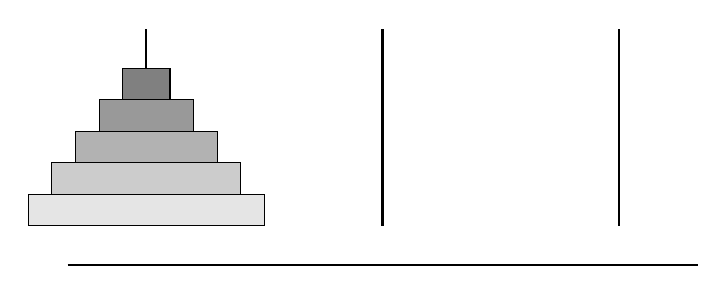
\begin{tikzpicture}
        % Draw the rods
            \draw[thick] (0,0) -- (0,2.5);
            \draw[thick] (3,0) -- (3,2.5);
            \draw[thick] (6,0) -- (6,2.5);
            
        % Draw the base
            \draw[thick] (-1,-0.5) -- (7,-0.5);
            
        % Draw the disks on the first rod
            \draw[fill=gray!20] (-1.5,0) rectangle (1.5,0.4);
            \draw[fill=gray!40] (-1.2,0.4) rectangle (1.2,0.8);
            \draw[fill=gray!60] (-0.9,0.8) rectangle (0.9,1.2);
            \draw[fill=gray!80] (-0.6,1.2) rectangle (0.6,1.6);
            \draw[fill=gray!100] (-0.3,1.6) rectangle (0.3,2);
    \end{tikzpicture}
    \caption{Illustration of the Hanoi Towers problem with disks.}
    \label{fig:hanoi}
\end{figure}

The Hanoi Towers problem consists of three rods and $n$ disks of different sizes. The disks are stacked in decreasing order of size on the first rod. The goal is to move all the disks to the third rod, following the rules:
\begin{itemize}
    \item Only one disk can be moved at a time.
    \item A disk can only be placed on top of a larger disk.
\end{itemize}

Let $h(n)$ be the number of moves required to move $n$ disks from the first to the third rod. The recurrence relation is:
\[
h(n) = 2h(n-1) + 1 = 2(2h(n-2) + 1) + 1 = 2^2 h(n-2) + 2 + 1 =
\]
\[
\dots = 2^n h(0) + 2^{n-1} + 2^{n-2} + \dots + 2^1 + 1
\]
\[
h(n) = 2^n - 1
\]

\subsection{Derangements as recurrence}
\begin{figure}[!h]
    \centering
    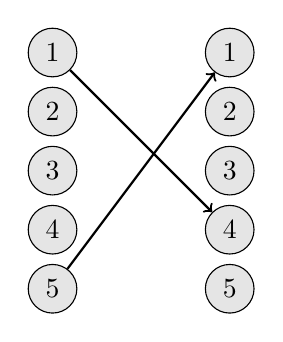
\begin{tikzpicture}[scale=1.5]
        % Nodes on the left
        \foreach \i in {1,2,3,4,5} {
            \node[circle, draw, fill=gray!20, minimum size=0.6cm] (L\i) at (0, 3-\i*0.5) {\i};
        }
        
        % Nodes on the right
        \foreach \i in {1,2,3,4,5} {
            \node[circle, draw, fill=gray!20, minimum size=0.6cm] (R\i) at (1.5, 3-\i*0.5) {\i};
        }
        
        % Arrows
        \draw[->, thick] (L1) -- (R4);
        \draw[->, thick] (L5) -- (R1);
    \end{tikzpicture}
    \label{fig:graph}
    \caption{Graph representation of a derangement.}
\end{figure}
\begin{itemize}
    \item Suppose $4 \rightarrow 1$ \quad $d(n-2)$ ways to derange the remaining elements.
    \item Suppose $4 \nrightarrow 1$ \quad $d(n-1)$ ways to derange the remaining elements.
\end{itemize}
\[
d(n) = (n-1)(d(n-1) + d(n-2))
\]

\subsection*{Example:}
Find a recurrence relation for the number of bit strings of length $n$ that do not contain two consecutive 0s. \\
Consider $n \geq 3$. Build the string from strings of length $n-1$.
\begin{itemize}
    \item If the last digit is 1, there are $d(n-1)$ ways to build the string.
    \item If the last digit is 0, the second-to-last digit must be 1. There are $d(n-2)$ ways to build the string.
\end{itemize}
\[
d(n) = d(n-1) + d(n-2) \quad \text{which is the Fibonacci sequence again!}
\]

\section{Linear Recurrence Relations}
\[
a_n = c_1 a_{n-1} + c_2 a_{n-2} + \dots + c_k a_{n-k} = \left\{a_n\right\}_{n=1}^{\infty}
\]
\[
\text{With } c_i \in \mathbb{R}, \quad c_k \neq 0 \quad \text{and} \quad k \geq 1 = \text{order of the recurrence relation}
\]

\[
1. \quad a_n = r^n, \quad r \in \mathbb{R}, \quad r \neq 0
\]
\[
r^n = c_1 r^{n-1} + c_2 r^{n-2} + \dots + c_k r^{n-k}
\]
\[
r^k - c_1 r^{k-1} - c_2 r^{k-2} - \dots - c_k = 0 \quad \rightarrow \text{Characteristic equation}
\]

\[
2. \quad \text{Superposition principle: the sum of solutions is also a solution} 
\]
\[
\{s_n\}, \{t_n\} \text{ are solutions } \rightarrow \{s_n + t_n\} \text{ is also a solution}
\]

\[
s_n = c_1 s_{n-1} + c_2 s_{n-2} + \dots + c_k s_{n-k}
\]
\[
t_n = c_1 t_{n-1} + c_2 t_{n-2} + \dots + c_k t_{n-k}
\]
\[
s_n + t_n = c_1 (s_{n-1} + t_{n-1}) + c_2 (s_{n-2} + t_{n-2}) + \dots + c_k (s_{n-k} + t_{n-k})
\]

\subsection{The $k = 2$ case}
\[
a_n = c_1 a_{n-1} + c_2 a_{n-2}, \quad c_2 \neq 0
\]
\[
a_0 = \alpha_0, \quad a_1 = \alpha_1, \quad \text{initial conditions}
\]

\[
\text{Then, } \quad r^2 - c_1 r - c_2 = 0
\implies \text{solutions } r_1 \neq r_2
\]

General solution:
\[
a_n = \beta_1 r_1^n + \beta_2 r_2^n
\]

Use the initial conditions to find $\beta_1$ and $\beta_2$.
\[
a_0 = \beta_1 + \beta_2 = \alpha_0 \quad \rightarrow \beta_2 = \alpha_0 - \beta_1
\]
\[
a_1 = \beta_1 r_1 + \beta_2 r_2 = \alpha_1 \quad \rightarrow \alpha_1 = \beta_1 r_1 + (\alpha_0 - \beta_1) r_2
\]

\[
\alpha_1 - \alpha_0 r_2 = \beta_1 (r_1 - r_2) \quad \rightarrow \beta_1 = \frac{\alpha_1 - \alpha_0 r_2}{r_1 - r_2}
\]

\[
\text{Then, } \quad \beta_2 = \alpha_0 - \frac{\alpha_1 - \alpha_0 r_2}{r_1 - r_2} = \frac{\alpha_0 r_1 - \alpha_1}{r_1 - r_2}
\]

\subsection*{Example:}
\[
a_n = a_{n-1} + 2a_{n-2}, \quad a_0 = 2, \quad a_1 = 7
\]
\[
r^2 - r - 2 = 0 \quad \rightarrow r_1 = 2, \quad r_2 = -1
\]
\[
a_n = \beta_1 2^n + \beta_2 (-1)^n
\]

\[
2 = \beta_1 + \beta_2 \quad \rightarrow \beta_2 = 2 - \beta_1
\]
\[
7 = 2 \beta_1 - \beta_2 \quad \rightarrow 7 = 2 \beta_1 - (2 - \beta_1) \quad \rightarrow \beta_1 = 3
\]
\[
\text{Then, } \quad \beta_2 = 2 - 3 = -1
\]

\[
a_n = 3 \cdot 2^n - (-1)^n
\]

\subsection*{Example: Fibonacci sequence}
\[
F_n = F_{n-1} + F_{n-2}, \quad F_0 = 0, \quad F_1 = 1
\]
\[
r^2 - r - 1 = 0 \quad \rightarrow r_1 = \frac{1 + \sqrt{5}}{2}, \quad r_2 = \frac{1 - \sqrt{5}}{2}
\]

\[
0 = \beta_1 + \beta_2 \quad \rightarrow \beta_2 = -\beta_1
\]
\[
1 = \beta_1 \frac{1 + \sqrt{5}}{2} - \beta_1 \frac{1 - \sqrt{5}}{2} \quad \rightarrow \beta_1 = \frac{1}{\sqrt{5}}
\]

\[
F_n = \frac{1}{\sqrt{5}} \left( \left( \frac{1 + \sqrt{5}}{2} \right)^n - \left( \frac{1 - \sqrt{5}}{2} \right)^n \right)
\]

\subsection*{Special case: $r_1 = r_2$}
\[
r^2 - c_1 r - c_2 = 0 \quad \rightarrow \text{With } r_1 = r_2 = r
\]
\[
\text{Then, the general solution is } a_n = \beta_1 r^n + \beta_2 n r^n
\]

\[
a_0 = \beta_1 = \alpha_0 \quad \rightarrow \beta_1 = \alpha_0
\]
\[
a_1 = \beta_1 r + \beta_2 r = \alpha_1 \quad \rightarrow \beta_2 = \frac{\alpha_1 - \alpha_0 r}{r}
\]

\subsection*{Example:}
\[
a_n = 6 a_{n-1} - 9 a_{n-2}, \quad a_0 = 1, \quad a_1 = 6
\]
\[
r^2 - 6r + 9 = 0 \quad \rightarrow r = 3
\]

\[
a_n = \beta_1 3^n + \beta_2 n 3^n
\]
\[
1 = \beta_1 \quad \rightarrow \beta_1 = 1
\]
\[
6 = 3 \beta_1 + 3 \beta_2 \quad \rightarrow 6 = 3 + 3 \beta_2 \quad \rightarrow \beta_2 = 1
\]

\[
a_n = 3^n + n 3^n
\]

\subsection{Theorem: Solution of degree $k$ recurrence relations with constant coefficients}
Let $a_n = c_1 a_{n-1} + c_2 a_{n-2} + \dots + c_k a_{n-k}, \quad c_i \in \mathbb{R}, \quad c_k \neq 0$ be a linear recurrence relation with constant coefficients.
Consider the characteristic equation:
\[
r^k - c_1 r^{k-1} - c_2 r^{k-2} - \dots - c_k = 0
\]
Assume it has different roots $r_1, r_2, \dots, r_t$, with multiplicities $m_1, m_2, \dots, m_t$, with $m_1 + m_2 + \dots + m_t = k$.
Then, the general solution is:

\[
a_n = (\beta_{10} + \beta_{11} n + \beta_{12} n^2 + \dots + \beta_{1m_1} n^{m_1-1}) r_1^n + \dots + (\beta_{t0} + \beta_{t1} n + \beta_{t2} n^2 + \dots + \beta_{tm_t} n^{m_t-1}) r_t^n
\]
\[
a_n = \sum_{i=1}^{t} \sum_{j=1}^{m_i} \beta_{ij} n^{j-1} r_i^n
\]

Given $k$ initial conditions $a_0 = \alpha_0, a_1 = \alpha_1, \dots, a_{k-1} = \alpha_{k-1}$, the coefficients $\beta_{ij}$ can be found by solving the system of linear equations.

\subsection*{Example:}
\[
a_n = -3 a_{n-1} - 3 a_{n-2} - a_{n-3}, \quad a_0 = 1, \quad a_1 = -2, \quad a_2 = -1
\]
\[
r^3 + 3r^2 + 3r + 1 = 0 \quad \rightarrow r = -1, \text{ with multiplicity } 3
\]

\[
a_n = (\beta_1 + \beta_2 n + \beta_3 n^2) (-1)^n
\]
\[
1 = \beta_1 \quad \rightarrow \beta_1 = 1
\]
\[
-2 = (1 + 2 \beta_2 + \beta_3) (-1) \quad \rightarrow 1 = \beta_2 + \beta_3 \quad \rightarrow \beta_2 = 3
\]
\[
-1 = (1 + 2 \beta_2 + 4 \beta_3) \quad \rightarrow -1 = 1 + 2 \beta_2 + 4 \beta_3 \quad \rightarrow \beta_3 = -2
\]

\[
a_n = 1 + 3n - 2n^2 (-1)^n
\]

\subsection{Nonhomogeneous Recurrence Relations}
\[
a_n = c_1 a_{n-1} + c_2 a_{n-2} + \dots + c_k a_{n-k} + F(n)
\]
\[
\text{With } F(n) \text{ a function of } n
\]

\paragraph{Theorem:}
The general solution of the nonhomogeneous case is:
\[
a_n = a_n^{(h)} + a_n^{(p)}
\]

Where $a_n^{(h)}$ is the general solution of the homogeneous case, with $F(n) = 0$, and $a_n^{(p)}$ is a particular solution of the nonhomogeneous case.

\subsection*{Example:}
\[
a_n = 3 a_{n-1} + 2n, \quad a_1 = 3
\]
\[
\text{Homogeneous: } \quad r - 3 = 0 \quad \rightarrow r = 3
\]
\[
\text{General solution: } \quad a_n^{(h)} = \beta 3^n
\]

\[
\text{Particular solution: assume } p_n = cn + d
\]
\[
cn + d = 3(c(n-1) + d) + 2n
\]
\[
cn + d = 3cn - 3c + 3d + 2n
\]
\[
c = 3c + 2 \implies c = -1
\]
\[
d = 3c + 3d \implies d = \frac{-3}{2}
\]

\[
\text{Particular solution: } \quad p_n = -n - \frac{3}{2}
\]
\[
\text{General solution: } \quad a_n = \beta 3^n - n - \frac{3}{2}
\]

\[
a_1 = 3 = \beta 3 - 1 - \frac{3}{2} 
\]
\[
3 \beta = \frac{11}{2} \implies \beta = \frac{11}{6}
\]

\[
a_n = \frac{11}{6} 3^n - n - \frac{3}{2}
\]

\subsection*{Example:}
\[
a_n = 5 a_{n-1} - 6 a_{n-2} + 7^n
\]
\[
r^2 - 5r + 6 = 0 \quad \rightarrow r = 2, 3
\]

\[
a_n^{(h)} = \beta_1 3^n + \beta_2 2^n
\]

\[
p_n = c 7^n = 5(c 7^{n-1}) - 6(c 7^{n-2}) + 7^n
\]
\[
49c = 35c - 6c + 49 \quad \rightarrow 20c = 49 \quad \rightarrow c = \frac{49}{20}
\]

\[
a_n = \beta_1 3^n + \beta_2 2^n + \frac{49}{20} 7^n
\]
\[
a_0 = 1, \quad a_1 = 2
\]

\[
1 = \beta_1 + \beta_2 + \frac{49}{20} \quad \rightarrow \beta_1 + \beta_2 = -\frac{29}{20}
\]
\[
2 = 3 \beta_1 + 2 \beta_2 + \frac{49}{20} \quad \rightarrow 3 \beta_1 + 2 \beta_2 = -\frac{11}{20}
\]
\[
\beta_1 = -\frac{9}{20}, \quad \beta_2 = -\frac{1}{4}
\]

\[
a_n = -\frac{9}{20} 3^n - \frac{1}{4} 2^n + \frac{49}{20} 7^n
\]

\subsection{Theorem: Particular solutions}
Let $a_n = c_1 a_{n-1} + c_2 a_{n-2} + \dots + c_k a_{n-k} + F(n)$ be a linear recurrence relation with constant coefficients and $F(n) = (b_t n^t + b_{t-1} n^{t-1} + \dots + b_1 n + b_0) s^n$.
Then, a particular solution if $s$ is not a root is:
\[
p_n = (d_t n^t + d_{t-1} n^{t-1} + \dots + d_1 n + d_0) s^n
\]

If $s$ is a root of the characteristic equation with multiplicity $m$, then the particular solution is:
\[
p_n = (d_t n^t + d_{t-1} n^{t-1} + \dots + d_1 n + d_0) s^n n^m
\]

\subsection*{Example:}
\[
a_n = 6 a_{n-1} - 9 a_{n-2} + F(n)
\]
\[
F(n) = 3^n, \quad F(n) = n 3^n, \quad F(n) = n^2 2^n, \quad F(n) = (1 + n) 2^n
\]

\[
r^2 - 6r + 9 = 0 \quad \rightarrow r = 3 \text{ with multiplicity } 2
\]

For $F(n) = 3^n$:
\[
p_n = d_0 n^2 3^n
\]

For $F(n) = n 3^n$:
\[
p_n = n^2 (d_1 n + d_0) \cdot 3^n
\]

For $F(n) = n^2 2^n$:
\[
p_n = (d_2 n^2 + d_1 n + d_0) 2^n
\]

For $F(n) = (1 + n) 2^n$:
\[
p_n = (d_1 n + d_0) 2^n
\]

\subsection{The $r = 1$ case}
\[
F(n) = (b_t n^t + b_{t-1} n^{t-1} + \dots + b_1 n + b_0) \cdot 1^n, \quad \text{with } r = 1 \text{ a root}
\]

\subsection*{Example:}
\[
a_n = \sum_{k = 1}^{n} k
\]
\[
a_n = a_{n-1} + n, \quad a_1 = 1
\]
\[
r - 1 = 0 \quad \rightarrow r = 1, \quad x_h = c 1^n = c
\]
\[
x_p = (p_1 n + p_0) \cdot n = p_1 n^2 + p_0 n
\]

\[
p_1 n^2 + p_0 n = p_1 (n-1)^2 + p_0 (n-1) + n
\]
\[
p_1 n^2 + p_0 n = p_1 n^2 - 2 p_1 n + p_1 + p_0 n - p_0 + n
\]
\[
0n + 0 = (1 - 2p_1) n + (p_1 - p_0)
\]

\[
p_1 = \frac{1}{2}, \quad p_0 = \frac{1}{2}
\]
\[
\implies a_n = c + \frac{n^2}{2} + \frac{n}{2}, \quad a_1 = 1 \implies c = 0
\]
\[
a_n = \frac{n^2 + n}{2} = \frac{n(n+1)}{2}
\]

\section{Generating Functions}
The generating function for a sequence $\{a_0, a_1, a_2, \dots\}$ of real numbers is the infinite formal series:
\[
G(x) = a_0 + a_1 x + a_2 x^2 + \dots a_k x^k = \sum_{k=0}^{\infty} a_k x^k
\]

\subsection*{Example:}
\[
a_k = k + 1 \quad \rightarrow \quad G(x) = 1 + 2x + 3x^2 + 4x^3 + \dots = \sum_{k=0}^{\infty} (k+1) x^k
\]

\[
a_k = 2^k \quad \rightarrow \quad G(x) = 1 + 2x + 4x^2 + 8x^3 + \dots = \sum_{k=0}^{\infty} 2^k x^k
\]

\subsection{Finite sequence}
\[
\{a_0, a_1, a_2, \dots, a_k\} \quad \rightarrow \quad G(x) = a_0 + a_1 x + a_2 x^2 + \dots + a_k x^k
\]

Which is like $a_i = 0$ for $i \geq k + 1$.

\subsection*{Example:}
\[
\{1, 1, 1, 1, 1, 1\} \quad \rightarrow \quad G(x) = 1 + x + x^2 + x^3 + x^4 + x^5 = \frac{x^6 - 1}{x - 1}
\]

\subsection*{Example:}
\[
a_k = \binom{n}{k} \quad \rightarrow \quad G(x) = (1 + x)^n = \sum_{k=0}^{n} \binom{n}{k} x^k
\]

\subsection{Frequent and important generating functions}

\begin{enumerate}
    \item $$\frac{1}{1 - x} = 1 + x + x^2 + x^3 + \dots = \sum_{k=0}^{\infty} x^k, \text{converges for } |x| < 1$$
          $$\frac{1}{1 - ax} = 1 + ax + a^2 x^2 + a^3 x^3 + \dots = \sum_{k=0}^{\infty} a^k x^k, \text{converges for } |x| < \frac{1}{|a|}$$
    \item $$\begin{cases}
                G_1(x) = \sum_{k = 0}^{\infty} a_kx^k \\
                G_2(x) = \sum_{k = 0}^{\infty} b_kx^k
            \end{cases} \implies 
            \begin{cases}
                G_1(x) + G_2(x) = \sum_{k = 0}^{\infty} (a_k + b_k)x^k \\
                G_1(x) \cdot G_2(x) = \sum_{k = 0}^{\infty} \left( \sum_{i = 0}^{k} a_i b_{k-i} \right)x^k
            \end{cases}$$
    \item $$\frac{1}{(1 - x)^2} = 1 + 2x + 3x^2 + 4x^3 + \dots = \frac{1}{1 - x} \cdot \frac{1}{1 - x} = \sum_{k = 0}^{\infty} x^k \cdot \sum_{j = 0}^{\infty} x^j = \sum_{k = 0}^{\infty} (k + 1)x^k$$
    \item $$\frac{1}{(1 - x)^2} = \frac{d}{dx} \left( \frac{1}{1 - x} \right) = \frac{d}{dx} \left( \sum_{k = 0}^{\infty} x^k \right) = \sum_{k = 0}^{\infty} kx^{k-1} = \sum_{k = 0}^{\infty} (k + 1)x^k$$
    \item $$\textbf{Definition:} \quad \binom{u}{k} = 
            \begin{cases}
                \dfrac{u(u-1)\dots(u-k+1)}{k!} & \text{if } k > 0 \\
                1 & \text{if } k = 0
            \end{cases}
            \quad \text{for } u \in \mathbb{R} \text{ and } k \in \mathbb{N}$$
            $$\text{If } u = -3 \text{ and } k = 2 \text{ then } \binom{-3}{2} = \frac{-3 \cdot -4}{2} = 6$$
            $$\text{If } u = \frac{1}{2} \text{ and } k = 3 \text{ then } \binom{\frac{1}{2}}{3} = \dfrac{\dfrac{1}{2} \cdot \dfrac{-1}{2} \cdot \dfrac{-3}{2}}{6} = \frac{1}{16}$$
            
            $$\textbf{Special case: } u \text{ is a negative integer } u = - n, \quad n \in \mathbb{N}$$
            $$\binom{-n}{r} = \frac{(-n)(-n-1)\dots(-n-r+1)}{r!} = \frac{(-1)^r n(n+1)\dots(n+r-1)}{r!} = $$
            $$= (-1)^r \binom{n+k-1}{k} = (-1)^r CR_n^r$$
            
            $$\textbf{Extended Binomial Theorem:} \quad (1 + x)^u = \sum_{k = 0}^{\infty} \binom{u}{k} x^k$$

            $$\textbf{Special case: } u = -n \text{ and } n \in \mathbb{N} $$
            $$(1 + x)^{-n} = \sum_{k = 0}^{\infty} \binom{-n}{k} x^k = \sum_{k = 0}^{\infty} (-1)^k \binom{n + k - 1}{k} x^k$$
            $$(1 - x)^{-n} = \sum_{k = 0}^{\infty} \binom{n + k - 1}{k} x^k$$ 
\end{enumerate}

\subsection{Applications of generating functions}
\subsection*{Example:}
Find the number of integer solutions of $x_1 + x_2 + x_3 = 17$ when $2 \leq x_1 \leq 5$, $3 \leq x_2 \leq 6$, and $3 \leq x_3 \leq 7$.
\[
G(x) = (x^2 + x^3 + x^4 + x^5)(x^3 + x^4 + x^5 + x^6)(x^3 + x^4 + x^5 + x^6 + x^7)
\]
We look for the coefficient of $x^{17}$ in $G(x)$.
\[
x^5 \cdot x^5 \cdot x^7 + x^5 \cdot x^6 \cdot x^6 + x^4 \cdot x^6 \cdot x^7 \rightarrow 3 \text{ solutions}
\]

\subsection*{Example:}
In how many ways can we distribute 8 identical cookies among 3 children so that each child recieves at least 2 and and no more than 4 cookies?
\[
G(x) = (x^2 + x^3 + x^4)^3 = x^6 (1 + x + x^2)^3 = x^6 (1 + 3x + 6x^2 + 7x^3 + 6x^4 + 3x^5 + x^6)
\]
\[
\text{Coefficient of } x^8 = 6 \text{ ways}
\]

\subsection*{Example:}
In how many ways can we gather $r$ euros using coins of 1 and 2 and notes of 5?
\[
G(x) = (1 + x + x^2 + \dots)(1 + x^2 + x^4 + \dots)(1 + x^5 + x^{10} + \dots) 
\]
For $r = 7$:
\[
(1 + x + x^2 + x^3 + x^4 + x^5 + x^6 + x^7)(1 + x^2 + x^4 + x^6)(1 + x^5) =
\]
\[
x^7 \cdot 1 \cdot 1 + x \cdot x^6 \cdot 1 + x^5 \cdot x^2 \cdot 1 + x^3 \cdot x^4 \cdot 1 + x^2 \cdot x^5 \cdot 1 + x^4 \cdot x^3 \cdot 1 + x^6 \cdot x^2 \cdot 1 = 6 \text{ ways}
\]

Same, but now order matters:

To insert $n$ coins or notes adding up to $r$ euros:
\[
(x + x^2 + x^5)^n, \quad \text{coefficient of } x^r
\]
\[
G(x) = 1 + (x + x^2 + x^5) + (x + x^2 + x^5)^2 + \dots = \frac{1}{1 - (x + x^2 + x^5)}
\]

\subsection*{Example:}
Suppose we have 3 green balls, 3 blue balls, 2 red balls and 1 white ball. How many ways are there to choose four of them?
\[
x_g + x_b + x_r + x_w = 4
\]
\[
G(x) = (1 + x + x^2 + x^3)(1 + x + x^2 + x^3)(1 + x + x^2) (1 + x) = (1 + x + x^2 + x^3)^2 (1 + x + x^2) (1 + x)
\]
\[
G(x) = \frac{1 - x^4}{1 - x} \cdot \frac{1 - x^4}{1 - x} \cdot \frac{1 - x^3}{1 - x} \cdot \frac{1 - x^2}{1 - x} = \frac{(1 - x^4)^2 (1 - x^3) (1 - x^2)}{(1 - x)^4} = 
\]
\[
= (1 - 2x^4)(1 - x^3)(1 - x^2) = (1 - x^2 - x^3 - 2x^4 + \dots)(1 + 4x + \binom{5}{2}x^2 + \binom{6}{3}x^3 + \binom{7}{4}x^4 + \dots) =
\]
\[
\binom{7}{4} - \binom{5}{2} - 4 - 2 = 19
\]
\[
\frac{1}{(1 - x)^4} = \sum_{n = 0}^{\infty} \binom{n + 3}{3} x^n = \binom{7}{4}
\]

\subsection*{Example:}
18 candies in 5 boxes with none empty, an even number of candies in each box, with no more than 10 candies in thee first two and 2 to 6 candies in the last three.
\[
G(x) = (x^2 + x^4 + x^6 + x^8 + x^{10})^2(x^2 + x^4 + x^6)^3 =
\]
\[
= x^4 (1 + x^2 + x^4 + x^6 + x^8)^2 x^6(1 + x^2 + x^4)^3 = x^{10} \frac{(1 - x^{10})^2}{(1 - x^2)^2} \frac{(1 - x^6)^3}{(1 - x^2)^3} = x^{10} \frac{(1 - x^{10})^2 (1 - x^6)^3}{(1 - x^2)^5}
\]
\[
\text{Coefficient of } x^{8}: \quad (1 - x^{10})^2 (1 - x^6)^3 \rightarrow (1 - 3x^6 + 3x^{12} - x^{18}) \rightarrow (1 - 3x^6)
\]
\[
\frac{1}{(1 - x^2)^5} = \sum_{n = 0}^{\infty} \binom{n + 4}{n} x^{2n}
\]
\[
(1 - 3x^6)\left(1 + 5x^2 + \binom{6}{2}x^4 + \binom{7}{3}x^6 + \binom{8}{4}x^8 + \dots\right) \rightarrow -15 + \binom{8}{4} = 55
\]

\subsection{Recurrence relations and generating functions}
\subsection*{Example:}
\[
a_k = 3a_{k-1}, \quad a_0 = 2
\]
\[
r = 3 \rightarrow a_k = c3^k \rightarrow a_k = 2 \cdot 3^k
\]

Now with:
\[
G(x) = \sum_{k = 0}^{\infty} a_k x^k 
\]
\[
G(x) - 3xG(x) = \sum_{k = 0}^{\infty} a_k x^k - 3 \sum_{k = 1}^{\infty} a_{k-1} x^k = a_0 + \sum_{k = 1}^{\infty} a_k x^k - 3 \sum_{k = 1}^{\infty} a_{k-1} x^k =
\]
\[
= 2 + \sum_{k = 1}^{\infty} (a_k - 3a_{k-1}) x^k = 2, \quad \text{since } a_k = 3a_{k-1}
\]
\[
G(x) = \frac{2}{1 - 3x} = 2 \sum_{k = 0}^{\infty} 3^k x^k \rightarrow a_k = 2 \cdot 3^k
\]

\subsection*{Example:}
\[
a_n = 8a_{n-1} + 10^{n-1}, \quad a_1 = 9, \quad n \geq 0
\]
\[
G(x) = \sum_{n = 1}^{\infty} a_n x^n
\]

Introduction of $a_0$: $a_1 = 8a_0 + 10^0 = 9 \rightarrow a_0 = 1$
\[
a_n x^n = 8a_{n-1} x^n + 10^{n-1} x^n
\]
\[
\sum_{n = 1}^{\infty} a_n x^n = 8 \sum_{n = 1}^{\infty} a_{n-1} x^{n} + \sum_{n = 1}^{\infty} 10^{n-1} x^n 
\]
\[
G(x) - a_0 = 8x \sum_{n = 1}^{\infty} a_{n-1} x^{n - 1} + x \sum_{n = 1}^{\infty} 10^{n-1} x^ {n-1} = 
\]
\[
= 8x \sum_{n = 0}^{\infty} a_n x^n + x \sum_{n = 0}^{\infty} 10^n x^n = 8xG(x) + \frac{x}{1 - 10x}
\]
\[ 
G(x) - a_0 = 8xG(x) + \frac{x}{1 - 10x} = \frac{1 - 9x}{1 - 10x}
\]
\[
G(x) = \frac{1 - 9x}{(1 - 10x)(1 - 8x)} 
\]
\[
G(x) = \frac{A}{1 - 8x} + \frac{B}{1 - 10x} = \frac{1}{2} \left( \frac{1}{1 - 8x} + \frac{1}{1 - 10x} \right) = 
\]
\[
= \frac{1}{2} \left( \sum_{n = 0}^{\infty} 8^n x^n + \sum_{n = 0}^{\infty} 10^n x^n \right) \rightarrow a_n = \frac{1}{2} (8^n + 10^n)
\]
Where $A = \frac{1}{2}$ and $B = \frac{1}{2}$, since
\[
1 - 9x = A(1 - 10x) + B(1 - 8x) \rightarrow 1 = A + B, \quad -9 = -10A - 8B
\]
\[
9 = 10A + 8 - 8A \rightarrow 1 = 2A \rightarrow A = \frac{1}{2}, \quad B = \frac{1}{2}
\]

\[
\textbf{Homogeneous: } r = 8 \rightarrow a_n^h = c8^n
\]
\[
a_p = D \cdot 10^n \rightarrow 10D = 8D + 1 \rightarrow D = \frac{1}{2}
\]
\[
a_n = c8^n + \frac{1}{2} \cdot 10^n
\]
\[
a_1 = 9 = c8 + 5 \rightarrow c = \frac{1}{2}
\]

\subsection*{Example:}
\[
a_n = 3a_{n-1} + n, \quad a_0 = 1, \quad n \geq 1
\]
\[
G(x) = \sum_{n = 0}^{\infty} a_n x^n
\]
\[
a_n x^n = 3a_{n-1} x^n + nx^n
\]
\[
\sum_{n = 1}^{\infty} a_n x^n = \sum_{n = 1}^{\infty} 3a_{n-1} x^n + \sum_{n = 1}^{\infty} nx^n
\]
\[
G(x) - a_0 = 3x \sum_{n = 1}^{\infty} a_{n-1} x^{n-1} + x \sum_{n = 1}^{\infty} nx^{n-1} = 3x \sum_{n = 0}^{\infty} a_n x^n + x \sum_{n = 0}^{\infty} nx^n
\]
\[
G(x) - 1 = 3xG(x) + x \sum_{n = 0}^{\infty} nx^n = 3xG(x) + x \frac{d}{dx} \left( \sum_{n = 0}^{\infty} x^n \right) = 3xG(x) + x \frac{d}{dx} \left( \frac{1}{1 - x} \right)
\]
\[
G(x) - 1 = 3xG(x) + x \frac{1}{(1 - x)^2} = 3xG(x) + \frac{x}{(1 - x)^2}
\]
\[
G(x) = \frac{1}{1 - 3x} + \frac{x}{(1 - x)^2(1 - 3x)} = \frac{A}{1 - x} + \frac{B}{(1 - x)^2} + \frac{C}{1 - 3x}
\]
\[
x = A(1 - x)(1 - 3x) + B(1 - 3x) + C(1 - x)^2 
\]

\[
\begin{cases}
    1 = B(1 - 3) \rightarrow B = -\frac{1}{2} \\
    \frac{1}{3} = C \frac{4}{9} \rightarrow C = \frac{3}{4} \\
    0 = A + B + C \rightarrow A = -\frac{1}{4}
\end{cases}
\]

\[
G(x) = \frac{7}{4} \frac{1}{1 - 3x} - \frac{1}{2} \frac{1}{(1 - x)^2} - \frac{1}{4} \frac{1}{1 - x}
\]
\[
G(x) = \sum_{n = 0}^{\infty} \left( \frac{7}{4} 3^n - \frac{1}{2} (n + 1) - \frac{1}{4} \right) 
\]

\subsection*{Example:}
\[
a_{n+2} - 5a_{n+1} + 6a_n = 2, \quad x_0 = 3, \quad x_1 = 7, \quad n \geq 0
\]
\[
G(x) = \sum_{n = 0}^{\infty} a_n x^n = 3 + 7x + \sum_{n = 2}^{\infty} a_n x^n
\]
Multiply by $x^{n+2}$:
\[
a_{n+2} x^{n+2} - 5a_{n+1} x^{n+2} + 6a_n x^{n+2} = 2x^{n+2}
\]
Sum over all allowed $n$:
\[
\sum_{n = 0}^{\infty} a_{n+2} x^{n+2} - 5 \sum_{n = 0}^{\infty} a_{n+1} x^{n+2} + 6 \sum_{n = 0}^{\infty} a_n x^{n+2} = 2 \sum_{n = 0}^{\infty} x^{n+2}
\]
Match the power of $x$ with the index of $a_n$ extracting as many factors $x$ as needed:
\[
\sum_{n = 0}^{\infty} a_{n+2} x^{n+2} - 5x \sum_{n = 0}^{\infty} a_{n+1} x^{n+1} + 6x^2 \sum_{n = 0}^{\infty} a_n x^n = 2x^2 \sum_{n = 0}^{\infty} x^n
\]
Shift the index of the sums:
\[
\sum_{n = 2}^{\infty} a_n x^n - 5x \sum_{n = 1}^{\infty} a_n x^n + 6x^2 \sum_{n = 0}^{\infty} a_n x^n = 2x^2 \sum_{n = 0}^{\infty} x^n
\]
Identify functions (use initial conditions as needed):
\[
G(x) - 3 - 7x = -5x(G(x) - 3) + 6x^2 G(x) = \frac{2x^2}{1 - x}
\]
Solve for $G(x)$:
\[
G(x) (1 - 5x + 6x^2) = 3 + 7x - 15x + \frac{2x^2}{1 - x} 
\]
\[
G(x) = \frac{3 - 8x}{1 - 5x + 6x^2} + \frac{2x^2}{(1 - x)(1 - 5x + 6x^2)}
\]
\[
G(x) = \frac{3 - 8x}{(1 - 2x)(1 - 3x)} + \frac{2x^2}{(1 - x)(1 - 2x)(1 - 3x)}
\]
\[
G(x) = \frac{2}{1 - 3x} + \frac{1}{1 - x} = 2 \sum_{n = 0}^{\infty} 3^n x^n + \sum_{n = 0}^{\infty} x^n
\]
\[
a_n = 2 \cdot 3^n + 1
\]

\subsection*{Example:}
A person has 6 friends: $\{A, B, C, D, E, F\}$. He wants to invite 4 of them home, but A and B cannot come together, and neihter can E and F, because of personal conflicts. If the invitation is made at random, what is the possibiliy that the dinner goes well?
\[
P = \frac{\text{number of good outcomes}}{\text{total number of groups of 4 friends}}
\]

\[
\text{Total number of groups of 4 friends: } \binom{6}{4} = 15
\]

\[
S_{AB} = \text{number of groups with A and B together} = \binom{4}{2} = 6
\]
\[
S_{EF} = \text{number of groups with E and F together} = \binom{4}{2} = 6
\]
\[
S_{ABEF} = \text{number of groups with A and B and E and F together} = \binom{2}{2} = 1
\]

\[
\text{Number of good outcomes: } 15 - 6 - 6 + 1 = 4
\]
\[
P = \frac{4}{15}
\]

\subsection*{Example:}
In how many ways can we order the letters A, E, M, O, Y, U in 6-letter strings without letter repetition that do not contain the word "ME" or "YOU"?
\[
\text{Total number of strings: } 6! = 720
\]

\[
S_{ME} = \text{number of strings with "ME"} = 5! = 120
\]
\[
S_{YOU} = \text{number of strings with "YOU"} = 4! = 24
\]
\[
S_{MEYOU} = \text{number of strings with "ME" and "YOU"} = 3! = 6
\]

\[
\text{Number of good strings: } 720 - 120 - 24 + 6 = 582
\]

\subsection*{Example:}
A message is made of 12 symbols in a specified order. To transmit it, you have to send 45 blanks along with the symbols, and every two symbols must be separated by at least 3 blanks. How many different messages can be sent?
\[
CR_{11}^{12} = \binom{11 + 12 - 1}{12} = \binom{22}{12} = 646646
\]

\subsection*{Example:}
How many subsets of 4 elements can be formed from elements of $\{1, 2, 3, \dots, 13, 14, 15\}$ such that no subset contains two consecutive numbers?
\[
\text{Subsets look like: } \{n_1, n_2, n_3, n_4\} \quad 1 \leq n_i \leq 15
\]
\[
\text{For non-consecutive numbers: } \{n_1, n_2, n_3, n_4\} \quad n_2 - n_1 \geq 2, \quad n_3 - n_2 \geq 2, \quad n_4 - n_3 \geq 2
\]
\[
\begin{cases}
    x_1 = n_1 \geq 1 \\
    x_2 = n_2 - n_1 \geq 2 \\
    x_3 = n_3 - n_2 \geq 2 \\
    x_4 = n_4 - n_3 \geq 2 \\
\end{cases} \implies 
n_4 = x_4 + x_3 + x_2 + x_1 \leq 15
\]
\[
\begin{cases}
    y_1 = x_1 - 1 \geq 0 \\
    y_2 = x_2 - 2 \geq 0 \\
    y_3 = x_3 - 2 \geq 0 \\
    y_4 = x_4 - 2 \geq 0 \\
\end{cases} \implies
y_4 + y_3 + y_2 + y_1 \leq 8
\]
\[
y_1 + y_2 + y_3 + y_4 + y_5 = 8
\]

\[
CR_5^8 = \binom{8 + 5 - 1}{8} = \binom{12}{8} = 495
\]

\subsection*{Example:}
How many ways are there to choose 25 objects from 7 categories so that there are no more than 6 and no fewer than 2 objects in each category?
\[
G(x) = (x^2 + x^3 + x^4 + x^5 + x^6)^7 = x^{14} (1 + x + x^2 + x^3 + x^4)^7 = x^{14} \left( \frac{1 - x^5}{1 - x} \right)^7
\]
We need the coefficient of $x^{11}$:
\[
(1 - x^5)^7 = 1 - 7x^5 + 21x^{10} - \dots
\]
\[
\left(\frac{1}{1 - x}\right)^7 = \sum_{n = 0}^{\infty} \binom{n + 6}{n} x^n = \binom{6}{0} + \binom{7}{1}x + \dots + \binom{12}{6}x^6 + \dots + \binom{17}{11}x^{11} + \dots
\]
So the coefficient of $x^{11}$ is:
\[
\binom{17}{11} - 7 \binom{12}{6} + 21 \binom{7}{1} = 6055
\]

\subsection*{Example:}
\[
a_{n + 2} - 2a_{n + 1} + a_n = 2^n, \quad a_0 = 1, \quad a_1 = 2
\]
\[
\text{Homogeneous: } r^2 - 2r + 1 = 0 \rightarrow r = 1 \rightarrow a_n^h = c_1 + c_2 n
\]
\[
a_n = c_1 + c_2 n + a_n^p
\]
\[
\text{Particular: } a_{n + 2} - 2a_{n + 1} + a_n = 2^n \rightarrow a_n^p = 2^n
\]
\[
a_n = c_1 + c_2 n + 2^n
\]
\[
a_0 = 1 = c_1 + 2^0 \rightarrow c_1 = 0
\]
\[
a_1 = 2 = c_2 + 2^1 \rightarrow c_2 = 0
\]
\[
a_n = 2^n
\]

\subsection*{Example:}
Given the recurrence relation:
\[
a_{n+2} - 2a_{n+1} + a_n = 2^n, \quad a_0 = 1, \quad a_1 = 2
\]

Multiplying both sides by \( x^n \) and summing over all \( n \):
\[
\sum_{n=0}^{\infty} a_{n+2} x^n - 2 \sum_{n=0}^{\infty} a_{n+1} x^n + \sum_{n=0}^{\infty} a_n x^n = \sum_{n=0}^{\infty} 2^n x^n
\]

Defining the generating function:
\[
G(x) = \sum_{n=0}^{\infty} a_n x^n
\]

We rewrite the summations:
\[
\sum_{n=0}^{\infty} a_{n+2} x^n = G(x) - a_0 - a_1 x
\]
\[
\sum_{n=0}^{\infty} a_{n+1} x^n = x \sum_{n=1}^{\infty} a_n x^{n-1} = x(G(x) - a_0)
\]

Using these, we derive:
\[
G(x) - 1 - 2x - 2x(G(x) - 1) + x^2 G(x) = x^2 \sum_{n=0}^{\infty} 2^n x^n = \frac{x^2}{1-2x}
\]
\[
G(x) \left[1 - 2x + x^2 \right] - 1 = \frac{x^2}{1-2x}
\]
\[
G(x) = \frac{1}{(1-x)^2} + \frac{x^2}{(1-2x)(1-x)^2} = \frac{1}{1-2x}
\]

Since:
\[
\frac{1}{1-2x} = \sum_{n=0}^{\infty} (2x)^n
\]

we conclude:
\[
a_n = 2^n
\]

\subsection*{Example:}
\begin{enumerate}
    \item How many words can be formed with at most 5 letters of WATER?
    \item How many of them do not contain W?
    \item How many of them contain neither W nor E?
    \item How many of them contain both W and E?
\end{enumerate}

For (i)
\[
P_5 + V(5,4) + V(5,3) + V(5,2) + V(5,1)
\]
\[
\frac{5!}{0!} + \frac{5!}{4!} + \frac{5!}{2!} + \frac{5!}{3!} + \frac{5!}{4!}
\]

For (ii):
\[
V(4,1) + V(4,2) + V(4,3) + P_4
\]

For (iii):
\[
V_3^1 + V_3^2 + P_3
\]

For (iv):
\[
P_2 + 3 P_3 + \binom{3}{2} P_4 + P_5
\]

\subsection*{Example:}
A soccer team has 3 Goalkeepers, 8 Defenders, 6 Midfielders, and 4 Forwards. The coach wants to pick up a team with 1 Goalkeeper, 5 Defenders, 3 Midfielders, and 2 Forwards. However, he does not want players MA and FB to play together. 

\vspace{0.5cm}
Total Teams:
\[
\binom{3}{1} \binom{8}{5} \binom{6}{3} \binom{4}{2}
\]

Forbidden Teams:
\[
\binom{3}{1} \binom{8}{5} \binom{5}{2} \binom{3}{1}
\]

Also Consider:
\[
\binom{5}{2} \binom{3}{2} \quad \text{(with A, not B)}
\]
\[
\binom{5}{3} \binom{3}{1} \quad \text{(with B, not A)}
\]
\[
\binom{5}{3} \binom{3}{2} \quad \text{(neither)}
\]

\subsection*{Example:}

Show that in any set of 9 natural numbers, none of which has a prime factor larger than 5, there must be two whose product is a perfect square.

We express a number \( n \) in terms of its prime factorization:
\[
n = 2^x 3^y 5^z
\]

Thus, allowed numbers can be characterized by the tuple \( (x, y, z) \mod 2 \).

If we have two numbers:
\[
n = 2^{x_1} 3^{y_1} 5^{z_1}, \quad m = 2^{x_2} 3^{y_2} 5^{z_2}
\]

Then their product:
\[
n \cdot m = 2^{x_1 + x_2} 3^{y_1 + y_2} 5^{z_1 + z_2}
\]

must be a perfect square, meaning \( x_1 + x_2 \), \( y_1 + y_2 \), and \( z_1 + z_2 \) must be even.
\[
\begin{cases}
x_1 + x_2 \equiv 0 \mod 2 \\
y_1 + y_2 \equiv 0 \mod 2 \\
z_1 + z_2 \equiv 0 \mod 2
\end{cases}
\]

Since \( x, y, z \) can each take values in \( \{0,1\} \), there are \( 2^3 = 8 \) possible different tuples \( (x, y, z) \mod 2 \). By the pigeonhole principle, in any set of 9 numbers, at least two must share the same tuple, ensuring their product is a perfect square.

\subsection*{Example:}
We want to make perfumes and we have 5 ingredients: 

\textit{Vanilla, Lavender, Orange, Wood, Grass}.

\begin{enumerate}
    \item How many of them do not contain Vanilla?
    \item How many do not contain Vanilla or Wood?
    \item How many of them contain both Vanilla and Wood?
    \item How many perfumes can we make with up to 5 essences?
\end{enumerate}

The number of perfumes with up to 5 ingredients is given by 1 less than the solutions of 
\[
n_v + n_l + n_o + n_w + n_g + v \leq 5
\]
\[
n_v + n_l + n_o + n_w + n_g + v = 5
\]
\[
CR(6, 5) - 1 = 251
\]

(i)
\[
1 \leq n_l + n_o + n_w + n_g \leq 5
\]
\[
CR(5, 5) - 1 = 125
\]

(ii)
\[
1 \leq n_l + n_o + n_g \leq 5
\]
\[
CR(4, 5) - 1 = 55
\]

(iii)
\[
251 - 125 - 125 + 55 = 56
\]

\subsection*{Example:}
How many ways are there to order \( w \) white balls and \( b \) black balls in a row such that there are exactly \( k+1 \) groups of black balls?

Using combinatorial grouping:
\[ CR_{k+1}^{b-(k+1)} = \binom{b-1}{b-k-1} \]
White balls separate groups, so:
\[ \binom{w+1}{w-k} \]

\section{Correspondences}
Correspondences are relationships between elements of two sets $A$ and $B$.

For example, let:
\[
A := \{\text{cities of the world}\}, \quad B := \{\text{countries of the world}\}
\]
\[
x \in A, \quad y \in B, \quad xRy \Longleftrightarrow x \text{ is the capital of } y
\]

$H(x,y)$ means that $x$ is something with respect to $y$.
\[
\textbf{Defining set: } \quad \{x \in U \mid H(x,y)\}
\]

\subsection{Definition}
Given two sets $A$ and $B$, a correspondence of relation between $A$ and $B$ is a subset $R$ of $A \times B$, defined as:
\[
R := \{(a,b) \in A \times B \mid H(a,b)\}
\]

\subsection*{Example:}
\[
A := \{1, 2, 3, 4, 5, 6\}, \quad R := \{(m,n) \in A \times A \mid m \text{ divides } n\}
\]
\[
(1,3) \in R, \quad (2,4) \in R, \quad (3,5) \notin R
\]

\subsection*{Example:}
\[
f(x) : \mathbb{R} \rightarrow \mathbb{R}^+, \quad x \rightarrow x^2
\]
\[
f := \{(x,y) \in \mathbb{R} \times \mathbb{R}^+ \mid y = x^2\}
\]

\subsection{Representation of correspondences}
\begin{enumerate}
    \item \textbf{Arrow diagram:} $R$ is represented by arrows from elements of $A$ to elements of $B$.
        \begin{figure}[h]
            \centering
            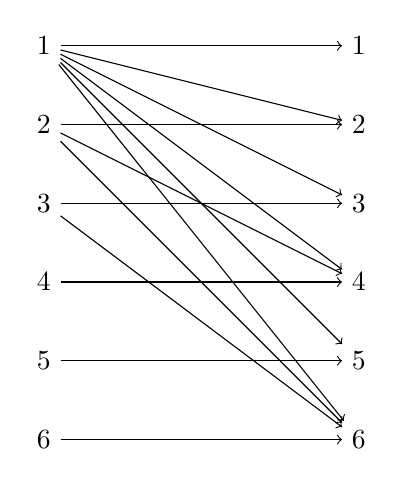
\begin{tikzpicture}
                \node (A1) at (0, 0) {1};
                \node (A2) at (0, -1) {2};
                \node (A3) at (0, -2) {3};
                \node (A4) at (0, -3) {4};
                \node (A5) at (0, -4) {5};
                \node (A6) at (0, -5) {6};

                \node (B1) at (4, 0) {1};
                \node (B2) at (4, -1) {2};
                \node (B3) at (4, -2) {3};
                \node (B4) at (4, -3) {4};
                \node (B5) at (4, -4) {5};
                \node (B6) at (4, -5) {6};

                \draw[->] (A1) -- (B1);
                \draw[->] (A1) -- (B2);
                \draw[->] (A1) -- (B3);
                \draw[->] (A1) -- (B4);
                \draw[->] (A1) -- (B5);
                \draw[->] (A1) -- (B6);

                \draw[->] (A2) -- (B2);
                \draw[->] (A2) -- (B4);
                \draw[->] (A2) -- (B6);

                \draw[->] (A3) -- (B3);
                \draw[->] (A3) -- (B6);

                \draw[->] (A4) -- (B4);

                \draw[->] (A5) -- (B5);

                \draw[->] (A6) -- (B6);
            \end{tikzpicture}
            \caption{Arrow diagram for the relation $R$ where $m$ divides $n$.}
            \label{fig:relation}
        \end{figure}
     \item \textbf{Binary matrix: } $R$ is represented by a matrix $M$ of dimensions $n \times n$ where $n = |A| = |B|$.
        \begin{figure}[h]
            \centering
            \begin{tabular}{c|cccccc}
            & 1 & 2 & 3 & 4 & 5 & 6 \\
            \hline
            1 & 1 & 1 & 1 & 1 & 1 & 1 \\
            2 & 0 & 1 & 0 & 1 & 0 & 1 \\
            3 & 0 & 0 & 1 & 0 & 0 & 1 \\
            4 & 0 & 0 & 0 & 1 & 0 & 1 \\
            5 & 0 & 0 & 0 & 0 & 1 & 0 \\
            6 & 0 & 0 & 0 & 0 & 0 & 1 \\
            \end{tabular}
            \caption{Binary matrix representation of the relation $R$ where $m$ divides $n$.}
            \label{fig:matrix}
        \end{figure}
    \item \textbf{Directed multigraph: } $R$ is represented by a directed multigraph where the vertices are elements of $A$ and $B$.
        \begin{figure}[h]
            \centering
            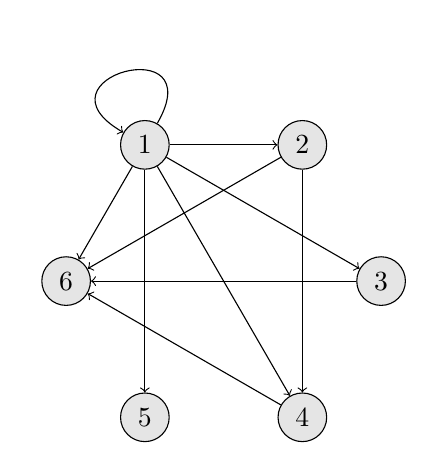
\begin{tikzpicture}
            % Nodes
            \node[circle, draw, fill=gray!20, minimum size=0.6cm] (A1) at (-1, 1.73) {1};
            \node[circle, draw, fill=gray!20, minimum size=0.6cm] (A2) at (1, 1.73) {2};
            \node[circle, draw, fill=gray!20, minimum size=0.6cm] (A3) at (2, 0) {3};
            \node[circle, draw, fill=gray!20, minimum size=0.6cm] (A4) at (1, -1.73) {4};
            \node[circle, draw, fill=gray!20, minimum size=0.6cm] (A5) at (-1, -1.73) {5};
            \node[circle, draw, fill=gray!20, minimum size=0.6cm] (A6) at (-2, 0) {6};

            % Arrows
            \draw[->, out=60, in=150, looseness=8] (A1) to (A1);
            \draw[->] (A1) -- (A2);
            \draw[->] (A1) -- (A3);
            \draw[->] (A1) -- (A4);
            \draw[->] (A1) -- (A5);
            \draw[->] (A1) -- (A6);

            \draw[->] (A2) -- (A4);
            \draw[->] (A2) -- (A6);

            \draw[->] (A3) -- (A6);

            \draw[->] (A4) -- (A6);
            \end{tikzpicture}
            \caption{Directed multigraph for the relation $R$ where $m$ divides $n$.}
            \label{fig:multigraph}
        \end{figure}
\end{enumerate}

\subsection{Domain and range of correspondences}
Let $R$ be a correspondence between $A$ and $B$, then:
\begin{enumerate}
    \item The \textbf{domain} of $R$ is the set of all elements of $A$ that are related to some element of $B$.
        \[ dom(R) = \{a \in A \mid (a,b) \in R \text{ for some } b \in B\} \subseteq A\]
    \item The \textbf{range} of $R$ is the set of all elements of $B$ that are related to some element of $A$.
        \[ ran(R) = \{b \in B \mid (a,b) \in R \text{ for some } a \in A\} \subseteq B\]
\end{enumerate}

\subsection*{Example:}
\[
A := \{1, 2, 3, 4, 5, 6\}, \quad mRn \Longleftrightarrow 2 \text{ divides } (m - n) 
\]
\[
m - n = 2k, \quad k \in \mathbb{Z} \rightarrow m = n (mod 2)
\]

\[
(1,1), (1,3), (1,5), (2,2), (2,4), (2,6), (3,1), (3,3), (3,5), 
\]
\[
(4,2), (4,4), (4,6), (5,1), (5,3), (5,5), (6,2), (6,4), (6,6)
\]

\subsection{Special relations}
\begin{enumerate}
    \item \textbf{Identity relation:} $I \subseteq A \times A$
        \[
        x,y \in A, \quad xIy \Longleftrightarrow x = y
        \]
    \item \textbf{Universal correspondence:} $U = A \times B$
    \item \textbf{Inverse correspondence:} If there exists $R \subseteq A \times B$, then: $R^{-1} \subseteq B \times A$
        \[
        R := \{(b,a) \in B \times A \mid (a,b) \in R\}
        \]
\end{enumerate}

\subsection{Properties of correspondences}
\begin{enumerate}
    \item \textbf{Reflexivity:} $R \subseteq A \times A$ is reflexive if and only if $(a,a) \in R$ for all $a \in A$.
    \item \textbf{Symmetry:} $R \subseteq A \times A$ is symmetric if and only if $(a,b) \in R \Leftrightarrow (b,a) \in R$.
    \item \textbf{Antisymmetry:} $R \subseteq A \times A$ is antisymmetric if and only if whenever \\ 
    $(a,b) \in R$ and $(b,a) \in R \implies a = b$.
    \item \textbf{Transitivity:} $R \subseteq A \times A$ is transitive if and only if whenever \\
    $(a,b) \in R$ and $(b,c) \in R \implies (a,c) \in R$.
\end{enumerate}

\subsection*{Example:}
\[
A := \{a, b, c, d\}, \quad R := \{(a,a), (a,b), (a,c), (b,a), (b,b), (b,c), (b,d), (d,d)\}
\]
\begin{enumerate}
    \item Reflexive: $(c,c) \notin R \implies R$ is not reflexive.
    \item Symmetric: $(a,c) \in R$, but $(c,a) \notin R \implies R$ is not symmetric.
    \item Antisymmetric: $(a,b) \in R, (b,a) \in R$, but $a \neq b \implies R$ is not antisymmetric.
    \item Transitive: $(a,b) \in R, (b,d) \in R$, but $(a,d) \notin R \implies R$ is not transitive.
\end{enumerate}

\subsection*{Example:}
\[
A := \{1, 2, 3, 4, 5, 6\}, \quad R := \{(m,n) \mid m \text{ divides } n\}
\]
\begin{enumerate}
    \item Reflexive: $\forall m \in A \implies m \text{ divides } m \implies R$ is reflexive.
    \item Symmetric: $m \text{ divides } n \implies n \text{ does not divide } m \implies R$ is not symmetric.
    \item Antisymmetric: $m \text{ divides } n, n \text{ divides } m \implies m = n \implies R$ is antisymmetric.
    \item Transitive: $m \text{ divides } n, n \text{ divides } p \implies m \text{ divides } p \implies R$ is transitive.
\end{enumerate}

\subsection*{Example:}
\[
A = \mathbb{N} \times \mathbb{N} = \{(a,b) \mid a,b \in \mathbb{N}\}, \quad R = \{\left((a,b), (c,d)\right) \mid a + d = b + c\}
\]
\begin{enumerate}
    \item Reflexive: $(a,b) + (b,a) = 2b = 2a \implies R$ is reflexive.
    \item Symmetric: $(a,b) + (c,d) = (c,d) + (a,b) \implies R$ is symmetric.
    \item Antisymmetric: $(a,b) + (c,d) = (c,d) + (a,b) \nRightarrow (a,b) = (c,d) \implies R$ is not antisymmetric.
    \item Transitive: $(a,b) + (c,d) = (c,d) + (e,f) \implies R$ is transitive.
\end{enumerate}

\subsection{Operations with correspondences}
\begin{enumerate}
    \item \textbf{Union:} $R \cup S = \{(a,b) \in A \times A \mid (a,b) \in R \text{ or } (a,b) \in S\}$
    \item \textbf{Intersection:} $R \cap S = \{(a,b) \in A \times A \mid (a,b) \in R \text{ and } (a,b) \in S\}$
\end{enumerate}

Both Union and Intersection preserve reflexivity and symmetry:
\begin{enumerate}
    \item If $R$ and $S$ are reflexive, then 
    \[
    \forall a \in A \quad (a,a) \in R \text{ and } (a,a) \in S \implies (a,a) \in R \cup S \text{ and } (a,a) \in R \cap S
    \]
    \item $R$ and $S$ are symmetric
    \[
    \text{If } (a,b) \in R \implies (b,a) \in R \text{ and } (c,d) \in S \implies (d,c) \in S 
    \]
\end{enumerate}

However, only Intersection preserves antisymmetry and transitivity.

\subsubsection{Counterexamples for the union}
\begin{enumerate}
    \item \textbf{Antisymmetry:} $R = \{(a,b)\}$ and $S = \{(b,a)\} \implies \text{antisymmetric, but }\\
    R \cup S = \{(a,b), (b,a)\} \text{ is not antisymmetric}$
    \item \textbf{Transitivity:} $R = \{(a,b)\}$ and $S = \{(b,c)\} \implies \text{transitive, but }\\
    R \cup S = \{(a,b), (b,c)\} \text{ is not transitive}$
\end{enumerate}

\subsection{Types of relations}
\begin{enumerate}
    \item \textbf{Equivalence relation:} A set $R \subseteq A \times A$ is an equivalence relation if and only if it is reflexive, symmetric, and transitive.
    \item \textbf{Order relation:} A set $R \subseteq A \times A$ is an order relation if and only if it is reflexive, antisymmetric, and transitive.
\end{enumerate}

\subsubsection{Equivalence relations}
\subsection*{Example:}
\[
A := \{\text{people living in Spain}\}, \quad R := \{(x,y) \mid x \text{ and } y \text{ live in the same municipality}\}
\]
\begin{enumerate}
    \item Reflexive: $x$ lives in the same municipality as $x$.
    \item Symmetric: If $x$ lives in the same municipality as $y$, then $y$ lives in the same municipality
    \item Transitive: If $x$ lives in the same municipality as $y$ and $y$ lives in the same municipality as $z$, then $x$ lives in the same municipality as $z$.
\end{enumerate}

\subsection*{Example:}
\[
A := \mathbb{R}^2 - \{(0,0)\}, \quad R := \{(x,y) \mid x \text{ and } y \text{ are on the same line through the origin}\}
\]
\begin{enumerate}
    \item Reflexive: $(0,0)$ is on the same line through the origin as $(0,0)$.
    \item Symmetric: If $x$ is on the same line through the origin as $y$, then $y$ is on the same line through the origin as $x$.
    \item Transitive: If $x$ is on the same line through the origin as $y$ and $y$ is on the same line through the origin as $z$, then $x$ is on the same line through the origin as $z$.
\end{enumerate}

\subsubsection{Equivalence class}
Let $A, \quad R \subset A \times A$ be an equivalence relation, then the class of equivalence of $x \in A$ is defined as 
\[
[x] = \{y \in A \mid (x,y) \in R\}
\]

The set of classes of equivalence of $R$ is a covering of $A$
\[
A = \bigcup_{x \in A}[x], \quad \text{remember } x \in [x] \text{ because of reflexivity and also } xRx \quad \forall x \in A
\]

Furthermore, $\bigcup_{x \in A}[x]$ is a partition of $A$

\paragraph{Theorem:} Let $A$ be a set, $R$ an equivalence,
\[
xRy \Longleftrightarrow [x] = [y]
\]

\paragraph{Proof:} $[x] = [y]$ \\
We need to prove:
\[
\begin{cases}
    [x] \subseteq [y] \\
    [y] \subseteq [x]
\end{cases}
\]
\[
\text{where } [x] = \{z \in A \mid xRz\}, \quad [y] = \{z \in A \mid yRz\}
\]

$[x] \subseteq [y]$: \\
Let $z \in [x]$, then $xRz \implies xRy \implies yRz \implies z \in [y]$.

Let $z \in [y]$, then $yRz \implies yRx \implies xRz \implies z \in [x]$.

The classes of equivalence form a partition of $A$.
\[
\forall x \in A, \quad x \in [x]
\]

If $[x]$ and $[y]$ have a common element, $z \in [x] \cap [y]$, then $[x] = [y]$.

\subsection{Quotient set}
Let $A$ be a set, $R$ an equivalence relation on $A$, then the quotient set of $A$ by $R$ is defined as:
\[
A/R = \{[x] \mid x \in A\}
\]

which means that $A/R$ is the set of all classes of equivalence of $A$ with respect to $R$.

\subsection*{Example:}
\[
A = \{a, b, c, d, e \}
\]
\[
R = \{(a,a), (b,b), (c,c), (d,d), (e,e), (a,b), (b,a), (a,c), (c,a), (b,c), (c,b)\}
\]

\[
A/R = \{\{a,b,c\}, \{d\}, \{e\} \}, \quad \text{where } [a] = [b] = [c]
\]

\begin{figure}[h]
    \centering
    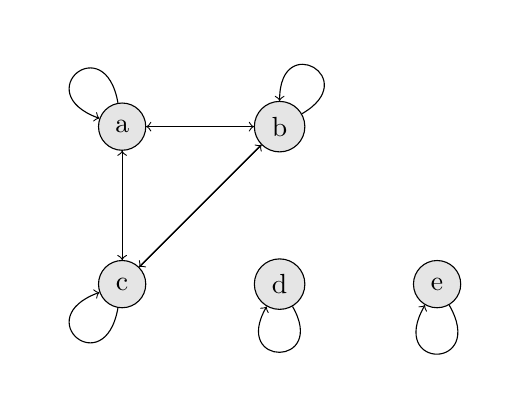
\begin{tikzpicture}
        % Nodes
        \node[circle, draw, fill=gray!20, minimum size=0.6cm] (A) at (0, 0) {a};
        \node[circle, draw, fill=gray!20, minimum size=0.6cm] (B) at (2, 0) {b};
        \node[circle, draw, fill=gray!20, minimum size=0.6cm] (C) at (0, -2) {c};
        \node[circle, draw, fill=gray!20, minimum size=0.6cm] (D) at (2, -2) {d};
        \node[circle, draw, fill=gray!20, minimum size=0.6cm] (E) at (4, -2) {e};

        % Arrows
        \draw[->, in = 160, out = 100, looseness = 8] (A) to (A);
        \draw[->, in = 90, out = 30, looseness = 7] (B) to (B);
        \draw[->, in = 200, out = 260, looseness = 8] (C) to (C);
        \draw[->, in = 240, out = 300, looseness = 7] (D) to (D);
        \draw[->, in = 240, out = 300, looseness = 8] (E) to (E);
        \draw[->] (A) -- (B);
        \draw[->] (A) -- (C);
        \draw[->] (B) -- (C);
        \draw[->] (C) -- (B);
        \draw[->] (B) -- (A);
        \draw[->] (C) -- (A);

    \end{tikzpicture}
    \caption{Directed multigraph for the relation $R$ where $a$, $b$, and $c$ are related to each other, and $d$, and $e$ are related to themselves.}
    \label{fig:multigraph2}
\end{figure}

\subsubsection{Example: Modular arithmetic}
\[
a, b \in \mathbb{Z}, \quad a \equiv b \mod n \Longleftrightarrow a - b = kn, \quad k \in \mathbb{Z}, \quad n \in \mathbb{N}
\]

\[
aRb \Longleftrightarrow a \equiv b \mod n \text{ is an equivalence relation}
\]

\[
\textbf{Reflexive: } a = a + 0n \implies a \equiv a \mod n \implies aRa
\]

\[
\textbf{Symmetric: } a \equiv b \mod n \implies a - b = kn 
\]
\[
\implies b - a = (-k)n \implies b \equiv a \mod n \implies aRb \implies bRa
\]

\[
\textbf{Transitive: } \begin{cases}
    a - b = kn \\
    b - c = ln
\end{cases} \implies a - c = (k + l)n \implies a \equiv c \mod n \implies aRc
\]

 \subsubsection{Equivalence classes: quotient set of $\mathbb{Z}$ by $n\mathbb{Z}$}
\[
[0] = \{x \in \mathbb{Z} \mid 0 - x = kn, \quad k \in \mathbb{Z}\} = \{x \in \mathbb{Z} \mid x = kn, \quad k \in \mathbb{Z}\}
\]

For $n \geq 2$:
\[
[1] = \{x \in \mathbb{Z} \mid 1 - x = kn, \quad k \in \mathbb{Z}\} = \{x \in \mathbb{Z} \mid 1 - x = kn, \quad k \in \mathbb{Z}\}
\]
\[ \vdots \]
\[
[n] = \{x \in \mathbb{Z} \mid n - x = kn, \quad k \in \mathbb{Z}\} = \{x \in \mathbb{Z} \mid x = kn, \quad k \in \mathbb{Z}\}
\]

\[
\mathbb{Z}/n\mathbb{Z} = \{[0], [1], \ldots, [n-1]\}
\]
\[
xy = (a + kn)(b + ln) = ab + (al + bk + kln)n
\]

In modular arithmetic: 
\[
[a] + [b] = [a + b], \quad [a] \cdot [b] = [a \cdot b]
\]

\[
x \in [a], \quad y \in [b] \implies x = a + kn, \quad y = b + ln
\]
\[
x + y = a + b + (k + l)n \implies x + y \in [a + b]
\]

\subsection{Order relations}
Let $A$ be a set, $R \subseteq A \times A$ an order relation. If $R$ is reflexive, antisymmetric, and transitive, then $R$ is an order relation.

\subsection*{Example:}
\[
R, \quad xRy \Longleftrightarrow x \leq y
\]

\begin{enumerate}
    \item Reflexive: $x \leq x$
    \item Antisymmetric: $x \leq y, y \leq x \implies x = y$
    \item Transitive: $x \leq y, y \leq z \implies x \leq z$
\end{enumerate}

\subsection*{Example:}
Let $A$ be a set, $P(A)$ the set of all subsets of $A$.
\[
B, C \in P(A), \quad B \subseteq C \Longleftrightarrow B \leq C
\]

\begin{enumerate}
    \item Reflexive: $B \subseteq B$
    \item Antisymmetric: $B \subseteq C, C \subseteq B \implies B = C$
    \item Transitive: $B \subseteq C, C \subseteq D \implies B \subseteq D$
\end{enumerate}

\subsection*{Example:}
\[
A = \{a,b,c\}, \quad P(A) = \{\emptyset, \{a\}, \{b\}, \{c\}, \{a,b\}, \{a,c\}, \{b,c\}, \{a,b,c\}\}
\]
\[
B, C \in P(A), \quad B \subseteq C \Longleftrightarrow B \leq C
\]
\[
\{a\} \leq \{a,b\}, \quad \text{but } \{a\} \nleq \{b,c\}
\]

\subsection{Theorem:}
Let $A$ be a set, with $\leq$ an order relation on $A$. Then:
\[
B \subseteq A \implies B \text{ is also an ordered set }
\]

\begin{enumerate}
    \item \textbf{Reflexive:} $x \in B \implies x \leq x$
    \item \textbf{Antisymmetric:} $x \leq y, y \leq x \implies x = y$
\end{enumerate}

\subsection{Notable elements in an order}
Let $A$ be a set, $\leq$ an order relation on $A$ and $B \subseteq A$. Then:
\begin{enumerate}
    \item $x \in A$ is an \textbf{upper bound} of $B$ if:
    \[
    \forall y \in B \implies y \leq x, \quad \text{(B is bounded from above)}
    \]
    \item $x \in A$ is a \textbf{lower bound} of $B$ if:
    \[
    \forall y \in B \implies x \leq y, \quad \text{(B is bounded from below)}
    \]
    Note: if $B$ is bounded from above and below, then $B$ is bounded.
    \item $x \in A$ is the \textbf{supremum} of $B$ if:
    \[
    x \leq y, \quad \forall y \in B, \quad \text{where } y \text{ is any upper bound of } B
    \]
    In case $x \in B$, then $x$ is the maximum of $B$.
    \item $x \in A$ is the \textbf{infimum} of $B$ if:
    \[
    y \leq x, \quad \forall y \in B, \quad \text{where } y \text{ is any lower bound of } B
    \]
    In case $x \in B$, then $x$ is the minimum of $B$.
    \item $y \in B$ is a \textbf{maximal element} of $B$ if:
    \[
    \nexists x \in B \text{ such that } y \leq x
    \]
    \item $y \in B$ is a \textbf{minimal element} of $B$ if:
    \[
    \nexists x \in B \text{ such that } y \geq x
    \]
\end{enumerate}

\paragraph{Theorem: } The supremum and infimum of a set are unique.
Let $\gamma, \gamma'$ be suprema of $B$, then:
\[
\gamma \leq \gamma' \text{ and } \gamma' \leq \gamma \implies \gamma = \gamma'
\]

\subsection*{Example:}
\[
A = \{a,b,c\}, \quad W = P(A) - A = \{\emptyset, \{a\}, \{b\}, \{c\}, \{a,b\}, \{a,c\}, \{b,c\}\}
\]
\[
W \subseteq P(A), \quad \emptyset \subset w \in W \implies \emptyset \leq w \quad \forall w \in W
\]
\[
\implies \emptyset \text{ is a lower bound of } W, \quad \emptyset \text{ is the infimum of } W, \quad \emptyset \text{ is the minimum of } W
\]

Also, $A$ is an upper bound of $W$, $A$ is the supremum of $W$, but $A$ is not the maximum of $W$.

The empty set is also a minimal element of $W$. However, there are three maximal elements in $W$: $\{a,b\}, \{a,c\}, \{b,c\}$. (Note that $A$ contains the but $A \notin W$).

\subsection*{Example:}
\[
A = \mathbb{N}, m \leq n \text{ if } m \text{ divides } n, \quad B = \{2,3,4,5,6,7,8\}
\]
\[
\text{The minimals of $B$ are } 2, 3, 5, 7, \text{ and the maximals are } 5,6,7,8
\]

Observe that 5 and 7 are both maximal and minimal elements of $B$.
\[
\text{The supremum of $B$ is the m.c.m. of all elements of $B$} = 2^3 \cdot 3 \cdot 5 \cdot 7 = 840, 
\]
\[
\text{and the infimum is the l.c.d. of all elements of $B$} = 1
\]

\subsection{Total order}
Let $A$ be a set, $\leq$ an order relation on $A$. $\leq$ is a total order if and only if:
\[
\forall x, y \in A \quad x \leq y \text{ or } y \leq x
\]

\subsection*{Examples:}
The usual order of $\mathbb{N}$ is a total order.

The alphabetical order of words is a total order.

\subsection{Types of order relations}
\begin{enumerate}
    \item \textbf{Well order:} A set is well oredered if $\forall a, b \in A$, $a \leq b$ or $b \leq a$.
    \item \textbf{Good order:} A set $A$ is good ordered if every non-empty subset of $A$ has a minimum.
\end{enumerate}

$\mathbb{N}$ is well ordered with respect to the usual order $\leq$.
$\mathbb{R}$ and $\mathbb{Q}$ are not well ordered.

\[
\text{Good order} \implies \text{Total order} \implies \text{Order}
\]

Let $A$ be a well ordered set, then every subset of $A$ has a minimum. In particular $\forall a, b \in A$, $\{a,b\} \subseteq A$ has a minimum which is the minimum of $a$ and $b$.

\subsubsection{Theorem:}
Let $A$ be an ordered set under $\mathcal{R}$, and $B$ an ordered set under $\mathcal{S}$. Then:
\begin{enumerate}
    \item $A$ is also an ordered set under $\mathcal{R}^{-1}$.
    \item $(A \times B, \mathcal{R} \times \mathcal{S})$ is also an ordered set, where:
    \[
    (a,b) \mathcal{R} \times \mathcal{S} (c,d) \Longleftrightarrow \begin{cases}
        a \mathcal{R} c \\
        b \mathcal{S} d
    \end{cases}
    \]
    \item $(A \times B, L)$, where $L$ is the lexicographic order, is also an ordered set.
    \[
    (a,b) L (c,d) \Longleftrightarrow \begin{cases}
        a \mathcal{R} c & \text{ if } a = c\\
        b \mathcal{S} d & \text{ otherwise}
    \end{cases}
    \]
\end{enumerate}

\subsubsection*{Examples:}
\[
\mathbb{N} \times \mathbb{N}, \quad \leq \text{ is the usual order}
\]
\[
(1,1) \leq (1,2), \quad (2,1) / (1,2)
\]

\[
\mathbb{N} \times \text{ dictionary}, \quad \leq \text{ is the alphabetical order}
\]
\[
(1, \text{fish}) \leq (3, \text{whale}), \quad (2, \text{shark}) / (7, \text{bird})
\]

\begin{enumerate}
    \item[3.] \textbf{Topological order: } \textbf{Theorem: } Let $A$ be a set, $\leq$ an order relation on $A$. Then there exists an order $\preceq$ that is total and is compatible with the order $\leq$.
    \[
    \forall a, b \in A, \quad a \leq b \implies a \preceq b 
    \]
    \textbf{Proof: } Let $a_1 \in A$, $a_1$ is a minimal element of $A$ with respect to $\leq$. Then, this will be the smallest element of $A$ with respect to $\preceq$ (it is the minimum of $A$). Now we look for a minimal element of $A - \{a_1\}$ with respect to $\leq$, $a_2$ such that $a_2 \preceq a_1$. We continue this process until we have a total order of $A$.
    \[
    a_1 \preceq a_2 \preceq a_3 \preceq \ldots \preceq a_n, \quad \text{where } n = |A|
    \]
\end{enumerate}

\subsection{Lattices}
Let $A$ be a set, $\leq$ an order relation on $A$. Then $(A, \leq)$ is a lattice if and only if both the supremum and infimum of any two elements of $A$ exist and belong to $A$.

\subsection*{Examples:}
Let $A = \{a,b,c\}$, under the usual order $\leq$ and consider $P(A)$ with an order given by inclusion $\subseteq$ (e.g. $\{a\} \subseteq \{a,b\}$). Then $(P(A), \subseteq)$ is a lattice.
\[
s_1, s_2 \in P(A), \quad inf \{s_1, s_2\} = s_1 \cap s_2 \in P(A), \quad sup \{s_1, s_2\} = s_1 \cup s_2 \in P(A)
\]

$\mathbb{N}$ with $n \leq m$ if $n$ divides $m$ is a lattice.
\[
inf \{n,m\} = gcd(n,m) \in \mathbb{N}, \quad sup \{n,m\} = lcm(n,m) \in \mathbb{N}
\]

\subsection{Hasse diagram}
Let $A$ be a set, $\leq$ an order relation on $A$. For $a, b \in A$, if $a < b$, and $\nexists$ $c \in A$ such that $a < c < b$, then we say that $b$ covers $a$.

\[
\text{Meaning of } a < b \quad \begin{cases}
    a \leq b \\
    a \neq b
\end{cases}
\]

In a Hasse diagram: 
\begin{enumerate}
    \item The elements of $A$ are represented by points.
    \item If $a < b$, then $a$ lies in a line below the line of $b$.
    \item If $b$ covers $a$, then there is a line connecting $a$ and $b$.
\end{enumerate}

\subsection*{Example:}
\[
A = \{1,2,3,4,5,6\}, \quad \text{division order}
\]

\begin{figure}[h]
    \centering
    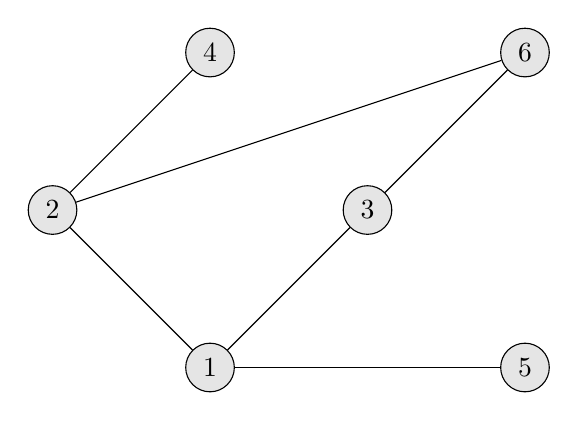
\begin{tikzpicture}
        % Nodes
        \node[circle, draw, fill=gray!20, minimum size=0.6cm] (1) at (2, -2) {1};
        \node[circle, draw, fill=gray!20, minimum size=0.6cm] (2) at (0, 0) {2};
        \node[circle, draw, fill=gray!20, minimum size=0.6cm] (3) at (4, 0) {3};
        \node[circle, draw, fill=gray!20, minimum size=0.6cm] (4) at (2, 2) {4};
        \node[circle, draw, fill=gray!20, minimum size=0.6cm] (5) at (6, -2) {5};
        \node[circle, draw, fill=gray!20, minimum size=0.6cm] (6) at (6, 2) {6};

        % Arrows
        \draw[-] (1) -- (2);
        \draw[-] (1) -- (3);
        \draw[-] (1) -- (5);
        \draw[-] (2) -- (4);
        \draw[-] (2) -- (6);
        \draw[-] (3) -- (6);
    \end{tikzpicture}
    \caption{Hasse diagram for the set $A = \{1,2,3,4,5,6\}$ with the division order.}
    \label{fig:hasse}
\end{figure}

\subsection*{Example:}
\[
P(A), \quad \subseteq \text{ order}, \quad A = \{a,b,c\}
\]

\begin{figure}[h!]
    \centering
    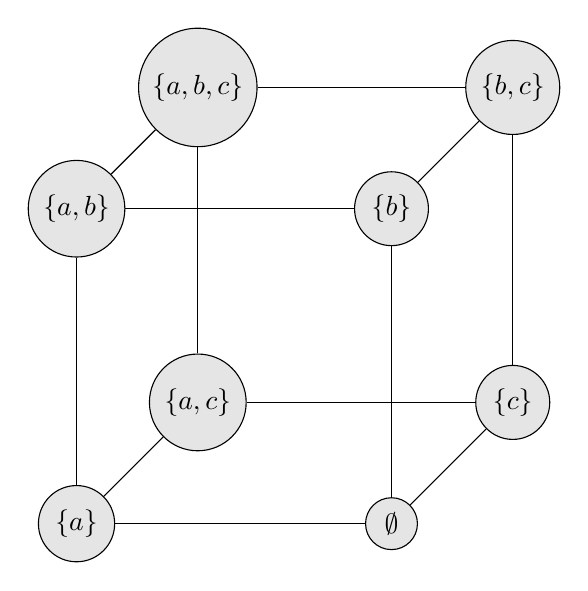
\begin{tikzpicture}
        % Nodes
        \node[circle, draw, fill=gray!20, minimum size=0.6cm] (empty) at (4, 0, 4) {$\emptyset$};
        \node[circle, draw, fill=gray!20, minimum size=0.6cm] (a) at (0, 0, 4) {$\{a\}$};
        \node[circle, draw, fill=gray!20, minimum size=0.6cm] (b) at (4, 4, 4) {$\{b\}$};
        \node[circle, draw, fill=gray!20, minimum size=0.6cm] (c) at (4, 0, 0) {$\{c\}$};
        \node[circle, draw, fill=gray!20, minimum size=0.6cm] (ab) at (0, 4, 4) {$\{a,b\}$};
        \node[circle, draw, fill=gray!20, minimum size=0.6cm] (ac) at (0, 0, 0) {$\{a,c\}$};
        \node[circle, draw, fill=gray!20, minimum size=0.6cm] (bc) at (4, 4, 0) {$\{b,c\}$};
        \node[circle, draw, fill=gray!20, minimum size=0.6cm] (abc) at (0, 4, 0) {$\{a,b,c\}$};

        % Lines
        \draw[-] (empty) -- (a);
        \draw[-] (empty) -- (b);
        \draw[-] (empty) -- (c);
        \draw[-] (a) -- (ab);
        \draw[-] (a) -- (ac);
        \draw[-] (b) -- (ab);
        \draw[-] (b) -- (bc);
        \draw[-] (c) -- (ac);
        \draw[-] (c) -- (bc);
        \draw[-] (ab) -- (abc);
        \draw[-] (ac) -- (abc);
        \draw[-] (bc) -- (abc);
    \end{tikzpicture}
    \caption{Hasse diagram for the set $P(A)$ with the inclusion order, where $A = \{a,b,c\}$.}
    \label{fig:hasse_inclusion}
\end{figure}

\subsection{Isomorphism of relations}
Let $A, B$ be sets, $R_A, R_B$ relations on $A$ and $B$, respectively. Then $A$ and $B$ are isomorphic if and only if there exists a bijective function $f: A \to B$ such that:
\[
\text{If } a, a' \in A, \quad aR_Aa' \Longleftrightarrow f(a)R_Bf(a')
\]

\subsection*{Example:}
\[
B = \{x_1x_2x_3 \mid x_i \in \{0,1\}\}
\]
\[
x_1x_2x_3 \leq y_1y_2y_3 \Longleftrightarrow \begin{cases}
    x_1 \leq y_1 \\
    x_2 \leq y_2 \\
    x_3 \leq y_3
\end{cases}
\]

\[
100 \leq 101, \quad \leq 110 / 101
\]
\[
x_1 = 0 \text{ if } a \notin W \in P(A), \quad x_1 = 1 \text{ if } a \in W \in P(A)
\]

\begin{figure}[h]
    \centering
    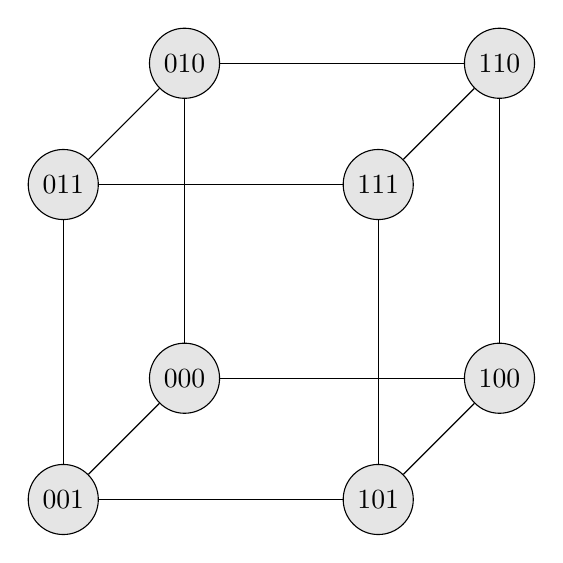
\begin{tikzpicture}
        % Nodes
        \node[circle, draw, fill=gray!20, minimum size=0.6cm] (000) at (0, 0, 0) {000};
        \node[circle, draw, fill=gray!20, minimum size=0.6cm] (001) at (0, 0, 4) {001};
        \node[circle, draw, fill=gray!20, minimum size=0.6cm] (010) at (0, 4, 0) {010};
        \node[circle, draw, fill=gray!20, minimum size=0.6cm] (011) at (0, 4, 4) {011};
        \node[circle, draw, fill=gray!20, minimum size=0.6cm] (100) at (4, 0, 0) {100};
        \node[circle, draw, fill=gray!20, minimum size=0.6cm] (101) at (4, 0, 4) {101};
        \node[circle, draw, fill=gray!20, minimum size=0.6cm] (110) at (4, 4, 0) {110};
        \node[circle, draw, fill=gray!20, minimum size=0.6cm] (111) at (4, 4, 4) {111};

        % Lines
        \draw[-] (000) -- (001);
        \draw[-] (000) -- (010);
        \draw[-] (000) -- (100);
        \draw[-] (001) -- (011);
        \draw[-] (001) -- (101);
        \draw[-] (010) -- (011);
        \draw[-] (010) -- (110);
        \draw[-] (011) -- (111);
        \draw[-] (100) -- (101);
        \draw[-] (100) -- (110);
        \draw[-] (101) -- (111);
        \draw[-] (110) -- (111);
    \end{tikzpicture}
    \caption{Hasse diagram for the set $B = \{x_1x_2x_3 \mid x_i \in \{0,1\}\}$ with the binary order.}
    \label{fig:hasse_binary}
\end{figure}

\subsection{Domain and range of a relation}
Obtain the domain and range of the correspondence in $\mathbb{N}$ defined by $xRy \Longleftrightarrow 2x + y = 16$.

A correspondence or relation is a subset of $A \times B$. The domain of a relation $R \subseteq A \times B$ is the set of all elements of $A$ that are related to some element of $B$. The range of $R$ is the set of all elements of $B$ that are related to some element of $A$.

\[
2x + y = 16 \implies y = 16 - 2x
\]
\[
x = 1 \implies y = 14 \implies (1,14) \in R, \quad 1R14
\]
\[
x = 2 \implies y = 12 \implies (2,12) \in R, \quad 2R12
\]
\[
x = 3 \implies y = 10 \implies (3,10) \in R, \quad 3R10
\]
\[
x = 4 \implies y = 8 \implies (4,8) \in R, \quad 4R8
\]
\[
x = 5 \implies y = 6 \implies (5,6) \in R, \quad 5R6
\]
\[
x = 6 \implies y = 4 \implies (6,4) \in R, \quad 6R4
\]
\[
x = 7 \implies y = 2 \implies (7,2) \in R, \quad 7R2
\]

The domain of $R$ is $\{1,2,3,4,5,6,7\}$ and the range is $\{2,4,6,8,10,12,14\}$.

\subsection*{Example:}
Let $A = \{a,b,c,d\}$ and $R = \{(a,a), (a,b), (a,c), (b,b), (b,c)\}$. Add elements to $R$ to make it:
\begin{enumerate}
    \item \textbf{Reflexive:} Add $(c,c), (d,d)$
    \item \textbf{Symmetric:} Add $(b,a), (c,a), (c,b)$
    \item \textbf{Antisymmetric:} No need to add anything, as it is already antisymmetric (no $x \neq y$ such that $xRy$ and $yRx$)
    \item \textbf{Transitive:} $(a,b), (b,c) \implies (a,c)$, which is already in $R$
\end{enumerate}

\subsection*{Example:}
Consider the correspondence $R \subseteq \mathbb{N} \times \mathbb{N}$:
\[
(m,n) R (p,q) \Longleftrightarrow m + q = n + p
\]

\begin{enumerate}
    \item Proof that $R$ is an equivalence relation.
    \item Find the equivalence classes of $(1,1)$, $(2,1)$, $(3,1)$, $(1,2)$ and $(1,3)$.
    \item Find the quotient set $\mathbb{N} \times \mathbb{N}/R$ and try to identify it with a known set.
\end{enumerate}

\begin{enumerate}
    \item \textbf{Reflexive:} $m + n = n + m$
    \item \textbf{Symmetric:} $m + q = n + p \implies n + p = m + q$
    \item \textbf{Transitive:} $m + q = n + p, \quad n + p = r + s \implies m + q = r + s$
\end{enumerate}

\[
(1,1) R (n,n) \implies [1,1] = \{(1,1), (2,2), (3,3), \ldots\}
\]
\[
(2,1) R (n+1,n) \implies [2,1] = \{(2,1), (3,2), (4,3), \ldots\}
\]
\[
(3,1) R (n+2,n) \implies [3,1] = \{(3,1), (4,2), (5,3), \ldots\}
\]
\[
(1,2) R (n-1,n) \implies [1,2] = \{(1,2), (2,3), (3,4), \ldots\}
\]
\[
(1,3) R (n-2,) \implies [1,3] = \{(1,3), (2,4), (3,5), \ldots\}
\]

\[
\mathbb{N} \times \mathbb{N}/R = \{[n,n+k], \quad \forall k \in \mathbb{Z}, \quad k > (-n)\} = [k] = \mathbb{Z}
\]

\subsection*{Example:}
Let $A$ be a set and let $R$ be a relation given by:
\[
    \renewcommand{\arraystretch}{1} % Adjust this value as needed
\begin{pmatrix}
    1 & 1 & 1 & 1 & 0 \\
    0 & 1 & 1 & 1 & 0 \\
    0 & 0 & 1 & 1 & 0 \\
    0 & 0 & 0 & 1 & 0 \\
    0 & 0 & 1 & 1 & 1
\end{pmatrix}
\]

\begin{enumerate}
    \item Prove that $R$ is an order relation in $A$.
    \item Find the domain and range of $R$.
    \item Draw the Hasse diagram of $R$.
    \item Find a topological order that contains $R$.
\end{enumerate}

\begin{enumerate}
    \item \textbf{Reflexive:} We have 1s in the diagonal, so it is reflexive.
    \item \textbf{Antisymmetric:} For every 1 in the matrix, there is a 0 in the symmetric position and vice versa, so it is antisymmetric.
    \item \textbf{Transitive:} By enumerating the elements, we can see that it is transitive.
\end{enumerate}

\[
\text{Domain: } \{a,b,c,d,e\}, \quad \text{Range: } \{a,b,c,d,e\}
\]

\[
\text{Minimals: } a \text{ and } e, \quad \text{Maximal: } d
\]

\begin{figure}[h]
    \centering
    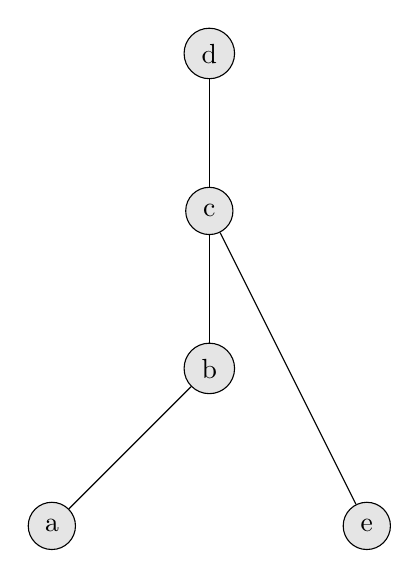
\begin{tikzpicture}
        % Nodes
        \node[circle, draw, fill=gray!20, minimum size=0.6cm] (1) at (0, 0, 0) {a};
        \node[circle, draw, fill=gray!20, minimum size=0.6cm] (2) at (2, 2, 0) {b};
        \node[circle, draw, fill=gray!20, minimum size=0.6cm] (3) at (2, 4, 0) {c};
        \node[circle, draw, fill=gray!20, minimum size=0.6cm] (4) at (2, 6, 0) {d};
        \node[circle, draw, fill=gray!20, minimum size=0.6cm] (5) at (4, 0, 0) {e};

        % Lines
        \draw[-] (1) -- (2);
        \draw[-] (2) -- (3);
        \draw[-] (3) -- (4);
        \draw[-] (3) -- (5);
    \end{tikzpicture}
    \caption{Hasse diagram for the set $A = \{a,b,c,d,e\}$ with the relation $R$.}
    \label{fig:hasse_relation}
\end{figure}

\[
\text{Topological order: } e \preceq a \preceq b \preceq c \preceq d
\]

\subsection*{Example:}
Let $A = \{2,3,5,6,10,30\}$ with the order relation $n \leq m$ if $n$ divides $m$. 
\begin{enumerate}
    \item Is $A$ totally ordered?
    \item Hasse diagram of $A$.
    \item Find the maximum, minimum, supremum and infimum of $A \subset \mathbb{N}$.
\end{enumerate}

An order is total if for every pair of elements $n, m \in A$, $n \leq m$ or $m \leq n$.
\[
2 \nmid 3, \quad 3 \nmid 2 \implies \text{ not totally ordered}
\]

\[
\text{Maximals: } 30, \quad \text{Minimals: } 2, 3, 5
\]

\begin{figure}[H]
    \centering
    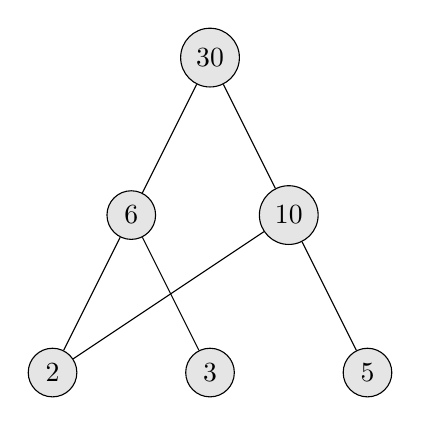
\begin{tikzpicture}
        % Nodes
        \node[circle, draw, fill=gray!20, minimum size=0.6cm] (2) at (0, 0, 0) {2};
        \node[circle, draw, fill=gray!20, minimum size=0.6cm] (3) at (2, 0, 0) {3};
        \node[circle, draw, fill=gray!20, minimum size=0.6cm] (5) at (4, 0, 0) {5};
        \node[circle, draw, fill=gray!20, minimum size=0.6cm] (6) at (1, 2, 0) {6};
        \node[circle, draw, fill=gray!20, minimum size=0.6cm] (10) at (3, 2, 0) {10};
        \node[circle, draw, fill=gray!20, minimum size=0.6cm] (30) at (2, 4, 0) {30};

        % Lines
        \draw[-] (2) -- (6);
        \draw[-] (2) -- (10);
        \draw[-] (3) -- (6);
        \draw[-] (5) -- (10);
        \draw[-] (6) -- (30);
        \draw[-] (10) -- (30);
    \end{tikzpicture}
    \caption{Hasse diagram for the set $A = \{2,3,5,6,10,30\}$ with the division order.}
    \label{fig:hasse_division}
\end{figure}

\[
\text{Supremum and maximum: } 30, \quad \text{Infimum but not minimum: } 1
\]

\subsection*{Example:}
Find the maximals, minimals, maximum and minimum of:

\begin{figure}[H]
    \centering
    \begin{minipage}{0.45\textwidth}
        \centering
        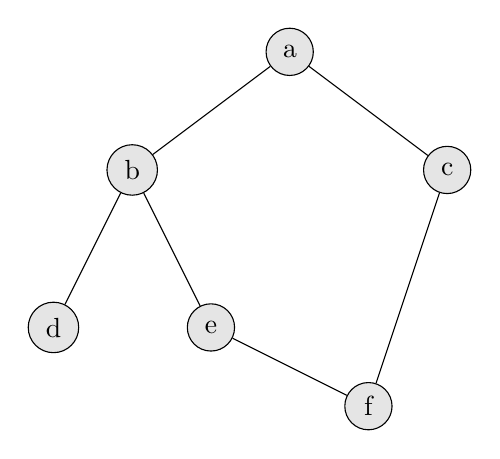
\begin{tikzpicture}
            % Nodes
            \node[circle, draw, fill=gray!20, minimum size=0.6cm] (1) at (3, 4.5, 0) {a};
            \node[circle, draw, fill=gray!20, minimum size=0.6cm] (2) at (1, 3, 0) {b};
            \node[circle, draw, fill=gray!20, minimum size=0.6cm] (3) at (5, 3, 0) {c};
            \node[circle, draw, fill=gray!20, minimum size=0.6cm] (4) at (0, 1, 0) {d};
            \node[circle, draw, fill=gray!20, minimum size=0.6cm] (5) at (2, 1, 0) {e};
            \node[circle, draw, fill=gray!20, minimum size=0.6cm] (6) at (4, 0, 0) {f};

            % Lines
            \draw[-] (1) -- (2);
            \draw[-] (1) -- (3);
            \draw[-] (2) -- (4);
            \draw[-] (2) -- (5);
            \draw[-] (3) -- (6);
            \draw[-] (5) -- (6);
        \end{tikzpicture}
        \caption{Hasse diagram for the set $A = \{a,b,c,d,e,f\}$ with the relation $R$.}
        \label{fig:hasse_relation2}
    \end{minipage}
    \hfill
    \begin{minipage}{0.45\textwidth}
        \centering
        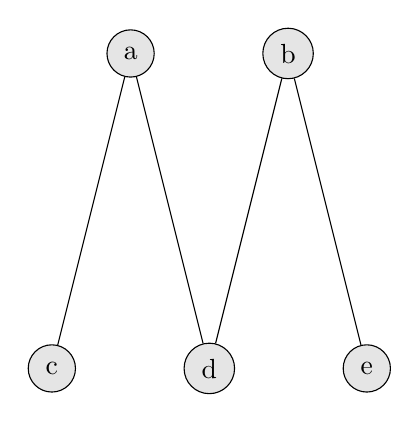
\begin{tikzpicture}
            % Nodes
            \node[circle, draw, fill=gray!20, minimum size=0.6cm] (1) at (1, 4, 0) {a};
            \node[circle, draw, fill=gray!20, minimum size=0.6cm] (2) at (3, 4, 0) {b};
            \node[circle, draw, fill=gray!20, minimum size=0.6cm] (3) at (0, 0, 0) {c};
            \node[circle, draw, fill=gray!20, minimum size=0.6cm] (4) at (2, 0, 0) {d};
            \node[circle, draw, fill=gray!20, minimum size=0.6cm] (5) at (4, 0, 0) {e};


            % Lines
            \draw[-] (1) -- (4);
            \draw[-] (1) -- (3);
            \draw[-] (2) -- (4);
            \draw[-] (2) -- (5);
        \end{tikzpicture}
        \caption{Another Hasse diagram for a different set $B = \{a,b,c,d,e\}$.}
        \label{fig:hasse_relation3}
    \end{minipage}
\end{figure}

For the first diagram:
\[
\text{Maximals and maximum: } a, \quad \text{Minimals: } d, f
\]

For the second diagram:
\[
\text{Maximals: } a, b, \quad \text{Minimals: } c, d, e
\]

\subsection*{Example:}
Find the upper bounds, lower bounds, supremum and infimum of the set $B = \{4,5,6\}$.

\begin{figure}[H]
    \centering
    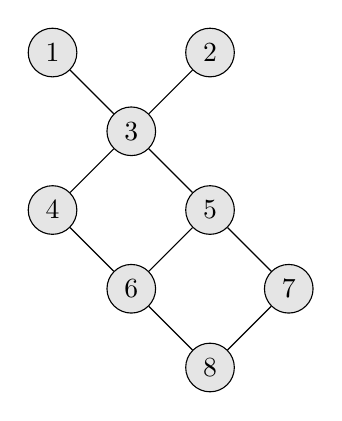
\begin{tikzpicture}
        % Nodes
        \node[circle, draw, fill=gray!20, minimum size=0.6cm] (1) at (0, 4, 0) {1};
        \node[circle, draw, fill=gray!20, minimum size=0.6cm] (2) at (2, 4, 0) {2};
        \node[circle, draw, fill=gray!20, minimum size=0.6cm] (3) at (1, 3, 0) {3};
        \node[circle, draw, fill=gray!20, minimum size=0.6cm] (4) at (0, 2, 0) {4};
        \node[circle, draw, fill=gray!20, minimum size=0.6cm] (5) at (2, 2, 0) {5};
        \node[circle, draw, fill=gray!20, minimum size=0.6cm] (6) at (1, 1, 0) {6};
        \node[circle, draw, fill=gray!20, minimum size=0.6cm] (7) at (3, 1, 0) {7};
        \node[circle, draw, fill=gray!20, minimum size=0.6cm] (8) at (2, 0, 0) {8};


        % Lines
        \draw[-] (1) -- (3);
        \draw[-] (2) -- (3);
        \draw[-] (3) -- (4);
        \draw[-] (3) -- (5);
        \draw[-] (4) -- (6);
        \draw[-] (5) -- (7);
        \draw[-] (6) -- (8);
        \draw[-] (7) -- (8);
        \draw[-] (5) -- (6);
    \end{tikzpicture}
    \caption{Hasse diagram for the set $B = \{4,5,6\}$ with the relation $R$.}
    \label{fig:hasse_relation4}
\end{figure}

\[
\text{Upper bounds: } 1,2,3 \quad \text{Lower bounds: } 8,6
\]
\[
\text{Supremum but not maximum (does not belong to } B \text{): } 3, \quad \text{Infimum and minimum: } 6
\]

\section{Graph theory}
A graph is a set of vertices $V$ and a set of edges $E \subseteq V \times V$. An edge is a pair of vertices.

\begin{center}
    \begin{figure}[H]
        \centering
        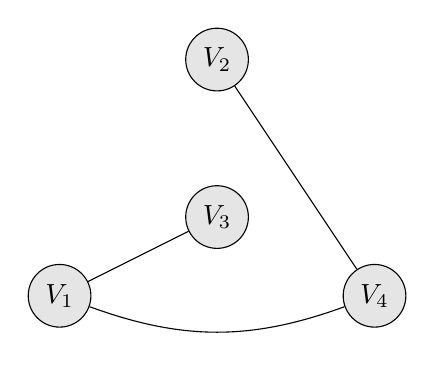
\begin{tikzpicture}
            % Nodes
            \node[circle, draw, fill=gray!20, minimum size=0.6cm] (1) at (0, 0, 0) {$V_1$};
            \node[circle, draw, fill=gray!20, minimum size=0.6cm] (2) at (2, 3, 0) {$V_2$};
            \node[circle, draw, fill=gray!20, minimum size=0.6cm] (3) at (2, 1, 0) {$V_3$};
            \node[circle, draw, fill=gray!20, minimum size=0.6cm] (4) at (4, 0, 0) {$V_4$};
    
            % Lines
            \draw[-] (1) -- (3);
            \draw[-, in = 200, out = 340, looseness = ] (1) to (4);
            \draw[-] (2) -- (4);
        \end{tikzpicture}
        \caption{Graph with vertices $V = \{V_1, V_2, V_3, V_4\}$ and edges $E = \{(V_1, V_3), (V_1, V_4), (V_2, V_4)\}$.}
    \end{figure}
\end{center}

\subsection{Directed graphs}
In a directed graph, the edges have a direction. We use the notation of the cartesian product $(v_i, v_j)$ to indicate that there is an edge from $v_i$ to $v_j$.

\subsubsection{Social networks}
\begin{center}
    \begin{figure}[H]
        \centering
        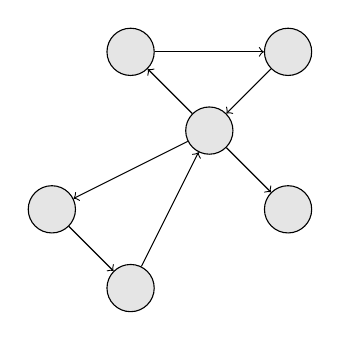
\begin{tikzpicture}
            % Nodes
            \node[circle, draw, fill=gray!20, minimum size=0.6cm] (1) at (2, 2, 0) {};
            \node[circle, draw, fill=gray!20, minimum size=0.6cm] (2) at (0, 1, 0) {};
            \node[circle, draw, fill=gray!20, minimum size=0.6cm] (3) at (1, 0, 0) {};
            \node[circle, draw, fill=gray!20, minimum size=0.6cm] (4) at (3, 1, 0) {};
            \node[circle, draw, fill=gray!20, minimum size=0.6cm] (5) at (1, 3, 0) {};
            \node[circle, draw, fill=gray!20, minimum size=0.6cm] (6) at (3, 3, 0) {};
    
            % Lines
            \draw[->] (1) -- (2);
            \draw[->] (3) -- (1);
            \draw[->] (2) -- (3);
            \draw[->] (1) -- (4);
            \draw[->] (1) -- (5);
            \draw[->] (5) -- (6);
            \draw[->] (6) -- (1);
            
        \end{tikzpicture}
        \caption{Directed graph representing a social network.}
    \end{figure}
\end{center}

\subsection{Multigraphs}
A multigraph allows for multiple edges between the same pair of vertices and loops (edges that start and end at the same vertex).

\subsection{Weighted graphs}
In a weighted graph, each edge has a weight associated with it.

\begin{center}
    \begin{figure}[H]
        \centering
        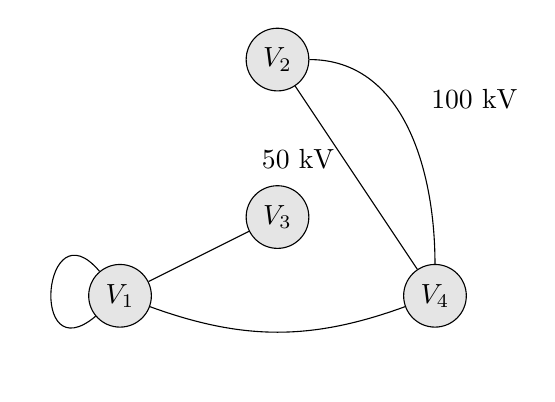
\begin{tikzpicture}
            % Nodes
            \node[circle, draw, fill=gray!20, minimum size=0.6cm] (1) at (0, 0, 0) {$V_1$};
            \node[circle, draw, fill=gray!20, minimum size=0.6cm] (2) at (2, 3, 0) {$V_2$};
            \node[circle, draw, fill=gray!20, minimum size=0.6cm] (3) at (2, 1, 0) {$V_3$};
            \node[circle, draw, fill=gray!20, minimum size=0.6cm] (4) at (4, 0, 0) {$V_4$};
    
            % Lines
            \draw[-] (1) -- (3);
            \draw[-, in = 220, out = 130, looseness = 5] (1) to (1);
            \draw[-, in = 200, out = 340] (1) to (4);
            \draw[-] (2) -- (4) node[pos=0.4, left] {50 kV};
            \draw[-, in = 90, out = 0, looseness = 1] (2) to (4);
            \node at (4.5, 2.5, 0) {100 kV};
        \end{tikzpicture}
        \caption{Graph with vertices $V = \{V_1, V_2, V_3, V_4\}$ and edges $E = \{(V_1, V_3), (V_1, V_4), (V_2, V_4)\}$.}
    \end{figure}
\end{center}

\subsubsection{Signed graphs}
In a signed graph, each edge has a weight that equals 1 or -1.

\subsection{Basic terminology and results}
\[
G(V,E), \quad \text{where } V = \{v_1, v_2, \ldots, v_n\}, \quad E = \{(v_i, v_j) \mid v_i, v_j \in V\}
\]

Two vertices $v_i, v_j \in G$ are adjacent (neighbors) if there is an edge between them (they form a pair). In a directed graph, we say that $v_i$ is adjacent to $v_j$ if there is an edge from $v_i$ to $v_j$.

Given a vertex $v_i \in V$, $G = (V,E)$ an undirected graph, the set of neighbors of $v$ is called the neighborhood of $v$ and is denoted by $N(v)$.
\[
A \subseteq V, \quad N(A) = \bigcup_{i = 1}^k N(v_i)
\]
\[
A = \{v_1, v_2, v_3\}
\]

The degree of a vertex $v_i$ is the number of edges incident to $v_i$. In a directed graph, we have the in-degree and out-degree of a vertex.
\[
\text{deg}(v) = |N(v)|
\]

\begin{center}
    \begin{figure}[H]
        \centering
        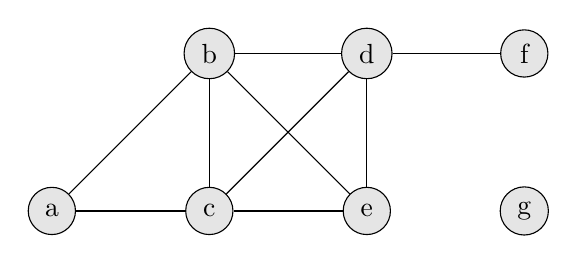
\begin{tikzpicture}
            % Nodes
            \node[circle, draw, fill=gray!20, minimum size=0.6cm] (1) at (0, 0, 0) {a};
            \node[circle, draw, fill=gray!20, minimum size=0.6cm] (2) at (2, 2, 0) {b};
            \node[circle, draw, fill=gray!20, minimum size=0.6cm] (3) at (2, 0, 0) {c};
            \node[circle, draw, fill=gray!20, minimum size=0.6cm] (4) at (4, 2, 0) {d};
            \node[circle, draw, fill=gray!20, minimum size=0.6cm] (5) at (4, 0, 0) {e};
            \node[circle, draw, fill=gray!20, minimum size=0.6cm] (6) at (6, 2, 0) {f};
            \node[circle, draw, fill=gray!20, minimum size=0.6cm] (7) at (6, 0, 0) {g};
    
            % Lines
            \draw[-] (1) -- (3);
            \draw[-] (1) -- (2);
            \draw[-] (2) -- (4);
            \draw[-] (3) -- (5);
            \draw[-] (4) -- (6);
            \draw[-] (2) -- (5);
            \draw[-] (3) -- (4);
            \draw[-] (2) -- (3);
            \draw[-] (4) -- (5);
        \end{tikzpicture}
        \caption{Graph with vertices $V = \{a,b,c,d,e,f,g\}$ and edges \\ $E = \{(a,c), (a,b), (b,d), (c,e), (d,f), (b,e), (c,d), (b,c), (d,e)\}$.}
    \end{figure}
\end{center}

$a$ is adjacent to $b$ and $c$, so $N(a) = \{b,c\}$.

Taking $A = \{b,c,e\}$, $N(A) = \{a,b,c,d,e\}$.

Taking $B = \{a,f\}$, $N(B) = \{b,c,d,e\}$.
\[
\text{deg}(a) = 2, \quad \text{deg}(b) = 4, \quad \text{deg}(c) = 3, \quad \text{deg}(d) = 3, \quad \text{deg}(e) = 3, \quad \text{deg}(f) = 1, \quad \text{deg}(g) = 0
\]

$f$ is called a leaf vertex, or a pendant node (a vertex with degree 1).

\subsection{Handshaking theorem}
Let $G = (V,E)$ be a graph. The sum of the degrees of all vertices is equal to twice the number of edges.
\[
\sum_{v \in V} \text{deg}(v) = 2|E|
\]

\subsubsection{Theorem}
Every undirected graph has an even number of vertices with odd degree.
\[
\sum_{v \in V} \text{deg}(v) = \sum_{v \in V_{\text{even}}} \text{deg}(v) + \sum_{v \in V_{\text{odd}}} \text{deg}(v) = 2|E| \implies \text{odd} + \text{even} = \text{even}
\]

For a directed graph, the sum of the in-degrees is equal to the sum of the out-degrees, where the in-degree (deg$^-$) of $v_i$ is the number of nodes that $v_i$ is adjacent from and the out-degree (deg$^+$) is the number of nodes that $v_i$ is adjacent to.

\subsubsection{Handshaking theorem for directed graphs}
\[
\sum_{v \in V} \text{deg}^-(v) = \sum_{v \in V} \text{deg}^+(v) = |E|
\]

\subsection{Special graphs (undirected)}
\begin{enumerate}
    \item \textbf{Complete graph ($K_n$):} A graph where every pair of vertices is adjacent. They are also called cliques.
    \[
    \text{Set of vertices } V, \quad |V| = n, \quad E = V \times V
    \]

    \begin{figure}[H]
        \centering
        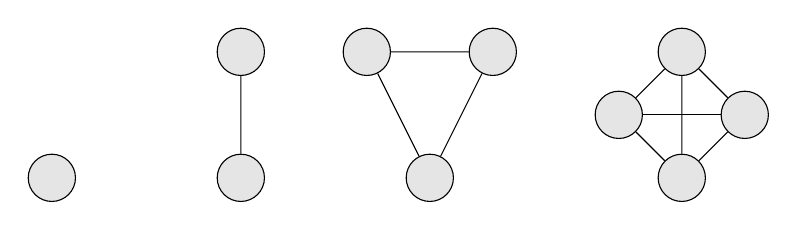
\begin{tikzpicture}[scale=0.8]
            % K_1
            \node[circle, draw, fill=gray!20, minimum size=0.6cm] (k1) at (0, 0) {};

            % K_2
            \node[circle, draw, fill=gray!20, minimum size=0.6cm] (k2a) at (3, 0) {};
            \node[circle, draw, fill=gray!20, minimum size=0.6cm] (k2b) at (3, 2) {};
            \draw[-] (k2a) -- (k2b);

            % K_3
            \node[circle, draw, fill=gray!20, minimum size=0.6cm] (k3a) at (6, 0) {};
            \node[circle, draw, fill=gray!20, minimum size=0.6cm] (k3b) at (5, 2) {};
            \node[circle, draw, fill=gray!20, minimum size=0.6cm] (k3c) at (7, 2) {};
            \draw[-] (k3a) -- (k3b);
            \draw[-] (k3b) -- (k3c);
            \draw[-] (k3c) -- (k3a);

            % K_4
            \node[circle, draw, fill=gray!20, minimum size=0.6cm] (k4a) at (10, 0) {};
            \node[circle, draw, fill=gray!20, minimum size=0.6cm] (k4b) at (9, 1) {};
            \node[circle, draw, fill=gray!20, minimum size=0.6cm] (k4c) at (11, 1) {};
            \node[circle, draw, fill=gray!20, minimum size=0.6cm] (k4d) at (10, 2) {};
            \draw[-] (k4a) -- (k4b);
            \draw[-] (k4b) -- (k4c);
            \draw[-] (k4c) -- (k4a);
            \draw[-] (k4a) -- (k4d);
            \draw[-] (k4b) -- (k4d);
            \draw[-] (k4c) -- (k4d);
        \end{tikzpicture}
        \caption{Complete graphs $K_1$, $K_2$, $K_3$, and $K_4$ aligned horizontally.}
        \label{fig:complete_graphs}
    \end{figure}
    \item \textbf{Cycle graph ($C_n, n \geq 3$):} A graph where the vertices form a cycle.
    \[
    V = \{v_1, v_2, \ldots, v_n\}, \quad E = \{(v_1, v_2), (v_2, v_3), \ldots, (v_{n-1}, v_n), (v_n, v_1)\}
    \]

    \begin{figure}[H]
        \centering
        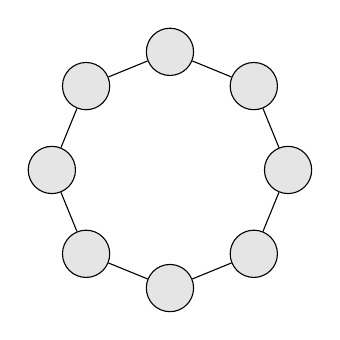
\begin{tikzpicture}[scale=1.5]
            % Nodes
            \node[circle, draw, fill=gray!20, minimum size=0.6cm] (1) at (0, 1) {};
            \node[circle, draw, fill=gray!20, minimum size=0.6cm] (2) at (0.71, 0.71) {};
            \node[circle, draw, fill=gray!20, minimum size=0.6cm] (3) at (1, 0) {};
            \node[circle, draw, fill=gray!20, minimum size=0.6cm] (4) at (0.71, -0.71) {};
            \node[circle, draw, fill=gray!20, minimum size=0.6cm] (5) at (0, -1) {};
            \node[circle, draw, fill=gray!20, minimum size=0.6cm] (6) at (-0.71, -0.71) {};
            \node[circle, draw, fill=gray!20, minimum size=0.6cm] (7) at (-1, 0) {};
            \node[circle, draw, fill=gray!20, minimum size=0.6cm] (8) at (-0.71, 0.71) {};

            % Edges
            \draw[-] (1) -- (2);
            \draw[-] (2) -- (3);
            \draw[-] (3) -- (4);
            \draw[-] (4) -- (5);
            \draw[-] (5) -- (6);
            \draw[-] (6) -- (7);
            \draw[-] (7) -- (8);
            \draw[-] (8) -- (1);
        \end{tikzpicture}
        \caption{Cycle graph $C_8$ representing an octagon.}
        \label{fig:octagon_cycle}
    \end{figure}
    \item \textbf{Wheel graph ($W_n$):} A cycle graph with an additional vertex that is adjacent to all other vertices.
    \begin{figure}[H]
        \centering
        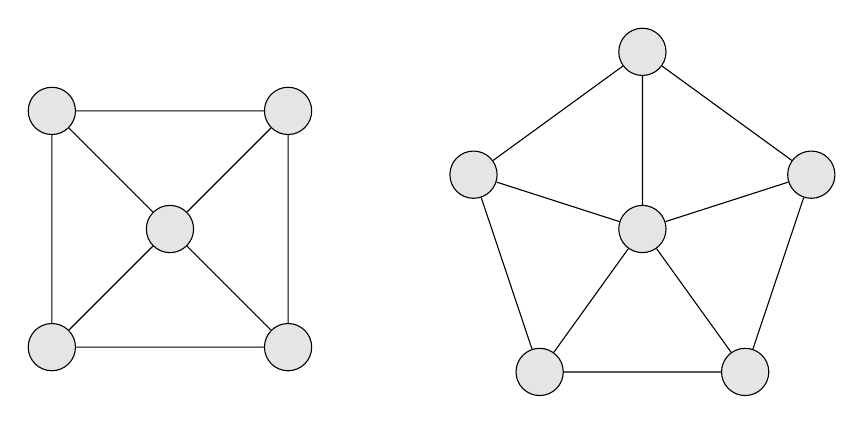
\begin{tikzpicture}[scale=1.5]
            % W_4
            \node[circle, draw, fill=gray!20, minimum size=0.6cm] (w4c) at (0, 0) {};
            \node[circle, draw, fill=gray!20, minimum size=0.6cm] (w4a) at (-1, 1) {};
            \node[circle, draw, fill=gray!20, minimum size=0.6cm] (w4b) at (1, 1) {};
            \node[circle, draw, fill=gray!20, minimum size=0.6cm] (w4d) at (1, -1) {};
            \node[circle, draw, fill=gray!20, minimum size=0.6cm] (w4e) at (-1, -1) {};
            \draw[-] (w4a) -- (w4b);
            \draw[-] (w4b) -- (w4d);
            \draw[-] (w4d) -- (w4e);
            \draw[-] (w4e) -- (w4a);
            \draw[-] (w4c) -- (w4a);
            \draw[-] (w4c) -- (w4b);
            \draw[-] (w4c) -- (w4d);
            \draw[-] (w4c) -- (w4e);

            % W_5 (Regular pentagon with center node)
            \node[circle, draw, fill=gray!20, minimum size=0.6cm] (w5c) at (4, 0) {};
            \node[circle, draw, fill=gray!20, minimum size=0.6cm] (w5a) at (4, 1.5) {};
            \node[circle, draw, fill=gray!20, minimum size=0.6cm] (w5b) at (5.43, 0.46) {};
            \node[circle, draw, fill=gray!20, minimum size=0.6cm] (w5d) at (4.87, -1.21) {};
            \node[circle, draw, fill=gray!20, minimum size=0.6cm] (w5e) at (3.13, -1.21) {};
            \node[circle, draw, fill=gray!20, minimum size=0.6cm] (w5f) at (2.57, 0.46) {};
            \draw[-] (w5a) -- (w5b);
            \draw[-] (w5b) -- (w5d);
            \draw[-] (w5d) -- (w5e);
            \draw[-] (w5e) -- (w5f);
            \draw[-] (w5f) -- (w5a);
            \draw[-] (w5c) -- (w5a);
            \draw[-] (w5c) -- (w5b);
            \draw[-] (w5c) -- (w5d);
            \draw[-] (w5c) -- (w5e);
            \draw[-] (w5c) -- (w5f);    
        \end{tikzpicture}
        \caption{Wheel graphs $W_4$ and $W_5$.}
        \label{fig:wheel_graphs}
    \end{figure}
    \item \textbf{Hypercube graph ($Q_n$):} A graph where each vertex represents a binary string of length $n$ and two vertices are adjacent if their binary strings differ in exactly one bit.
    \[
    E = \{(s_i, s_j) \mid s_i, s_j \in V, \text{ and } s_i, s_j \text{ differ in exactly one bit (position)}\}
    \]
    \begin{figure}[H]
        \centering
        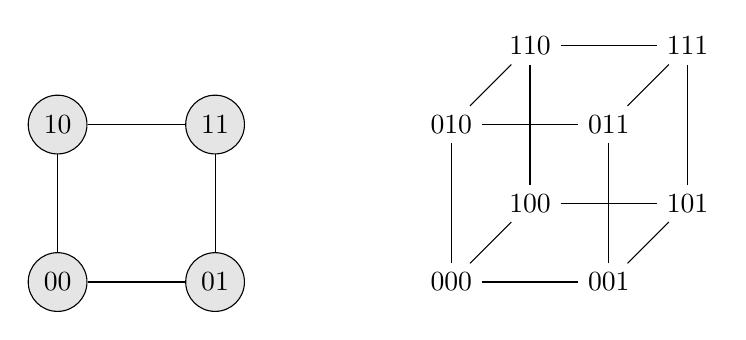
\begin{tikzpicture}
        % Q2 (Hypercube graph with n=2)
        \node[circle, draw, fill=gray!20, minimum size=0.4cm] (q2a) at (0, 0) {00};
        \node[circle, draw, fill=gray!20, minimum size=0.4cm] (q2b) at (2, 0) {01};
        \node[circle, draw, fill=gray!20, minimum size=0.4cm] (q2c) at (0, 2) {10};
        \node[circle, draw, fill=gray!20, minimum size=0.4cm] (q2d) at (2, 2) {11};
        \draw[-] (q2a) -- (q2b);
        \draw[-] (q2a) -- (q2c);
        \draw[-] (q2b) -- (q2d);
        \draw[-] (q2c) -- (q2d);

        % Q3 (Hypercube graph with n=3, represented as a cube)
        \node (q3a) at (5, 0) {000};
        \node (q3b) at (7, 0) {001};
        \node (q3c) at (5, 2) {010};
        \node (q3d) at (7, 2) {011};
        \node (q3e) at (6, 1) {100};
        \node (q3f) at (8, 1) {101};
        \node (q3g) at (6, 3) {110};
        \node (q3h) at (8, 3) {111};
        \draw[-] (q3a) -- (q3b);
        \draw[-] (q3a) -- (q3c);
        \draw[-] (q3b) -- (q3d);
        \draw[-] (q3c) -- (q3d);
        \draw[-] (q3e) -- (q3f);
        \draw[-] (q3e) -- (q3g);
        \draw[-] (q3f) -- (q3h);
        \draw[-] (q3g) -- (q3h);
        \draw[-] (q3a) -- (q3e);
        \draw[-] (q3b) -- (q3f);
        \draw[-] (q3c) -- (q3g);
        \draw[-] (q3d) -- (q3h);
        \end{tikzpicture}
        \caption{Hypercube graphs $Q_2$ and $Q_3$.}
        \label{fig:hypercube_graphs}
    \end{figure}
\end{enumerate}

\subsection{Bipartite graphs (undirected)}
A graph $G = (V,E)$ is bipartite if the set of vertices can be partitioned into two disjoint sets $V_1$ and $V_2$ such that every edge connects a vertex in $V_1$ to a vertex in $V_2$.
\[
V = V_1 \cup V_2, \quad V_1 \cap V_2 = \emptyset, \quad \forall (v_i, v_j) \in E, \quad v_i \in V_1, \quad v_j \in V_2
\]

\begin{figure}[H]
    \centering
        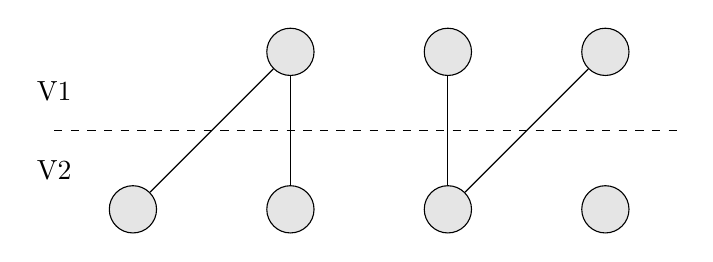
\begin{tikzpicture}
            % Nodes
            \node[circle, draw, fill=gray!20, minimum size=0.6cm] (1) at (0, 0) {};
            \node[circle, draw, fill=gray!20, minimum size=0.6cm] (2) at (2, 2) {};
            \node[circle, draw, fill=gray!20, minimum size=0.6cm] (3) at (2, 0) {};
            \node[circle, draw, fill=gray!20, minimum size=0.6cm] (4) at (4, 2) {};
            \node[circle, draw, fill=gray!20, minimum size=0.6cm] (5) at (4, 0) {};
            \node[circle, draw, fill=gray!20, minimum size=0.6cm] (6) at (6, 2) {};
            \node[circle, draw, fill=gray!20, minimum size=0.6cm] (7) at (6, 0) {};
    
            % Edges
            \draw[-] (1) -- (2);
            \draw[-] (2) -- (3);
            \draw[-] (4) -- (5);
            \draw[-] (5) -- (6);
            
            % Dotted line dividing the two parts
            \draw[dashed] (-1, 1) -- (7, 1);
            \node at (-1, 1.5) {V1};
            \node at (-1, 0.5) {V2};
        \end{tikzpicture}
    \caption{Bipartite graph with vertices $V = \{1,2,3,4,5,6,7\}$ and edges \\ $E = \{(1,2), (2,3), (4,5), (5,6)\}$.}
\end{figure}

\subsubsection{Theorem}
A graph is bipartite if and only if every vertex can be assigned one of two colors such that no two adjacent vertices have the same color.
\begin{figure}[H]
    \centering
    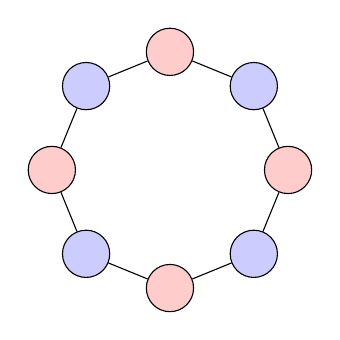
\begin{tikzpicture}[scale=1.5]
        % Nodes
        \node[circle, draw, fill=red!20, minimum size=0.6cm] (1) at (0, 1) {};
        \node[circle, draw, fill=blue!20, minimum size=0.6cm] (2) at (0.71, 0.71) {};
        \node[circle, draw, fill=red!20, minimum size=0.6cm] (3) at (1, 0) {};
        \node[circle, draw, fill=blue!20, minimum size=0.6cm] (4) at (0.71, -0.71) {};
        \node[circle, draw, fill=red!20, minimum size=0.6cm] (5) at (0, -1) {};
        \node[circle, draw, fill=blue!20, minimum size=0.6cm] (6) at (-0.71, -0.71) {};
        \node[circle, draw, fill=red!20, minimum size=0.6cm] (7) at (-1, 0) {};
        \node[circle, draw, fill=blue!20, minimum size=0.6cm] (8) at (-0.71, 0.71) {};

        % Edges
        \draw[-] (1) -- (2);
        \draw[-] (2) -- (3);
        \draw[-] (3) -- (4);
        \draw[-] (4) -- (5);
        \draw[-] (5) -- (6);
        \draw[-] (6) -- (7);
        \draw[-] (7) -- (8);
        \draw[-] (8) -- (1);

        % Labels
    \end{tikzpicture} \quad \quad \quad
    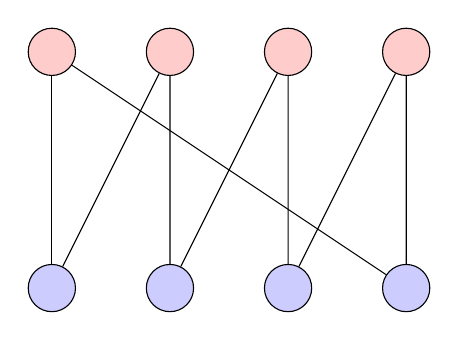
\begin{tikzpicture}[scale=1.5]
        % Nodes
        \node[circle, draw, fill=red!20, minimum size=0.6cm] (1) at (0, 2) {};
        \node[circle, draw, fill=blue!20, minimum size=0.6cm] (2) at (0, 0) {};
        \node[circle, draw, fill=red!20, minimum size=0.6cm] (3) at (1, 2) {};
        \node[circle, draw, fill=blue!20, minimum size=0.6cm] (4) at (1, 0) {};
        \node[circle, draw, fill=red!20, minimum size=0.6cm] (5) at (2, 2) {};
        \node[circle, draw, fill=blue!20, minimum size=0.6cm] (6) at (2, 0) {};
        \node[circle, draw, fill=red!20, minimum size=0.6cm] (7) at (3, 2) {};
        \node[circle, draw, fill=blue!20, minimum size=0.6cm] (8) at (3, 0) {};

        % Edges
        \draw[-] (1) -- (2);
        \draw[-] (2) -- (3);
        \draw[-] (3) -- (4);
        \draw[-] (4) -- (5);
        \draw[-] (5) -- (6);
        \draw[-] (6) -- (7);
        \draw[-] (7) -- (8);
        \draw[-] (8) -- (1);

        % Labels
    \end{tikzpicture}
    \caption{Bipartite graph $C_8$ (octagon) and alternative representation with colored vertices.}
\end{figure}

$K_{n,m}$  is the complete bipartite graph with $n$ vertices in $V_1$, $m$ vertices in $V_2$ and all possible edges between $V_1$ and $V_2$.
% K_{2,3} (Complete bipartite graph with 2 vertices in V1 and 3 in V2)
\begin{figure}[H]
    \centering
    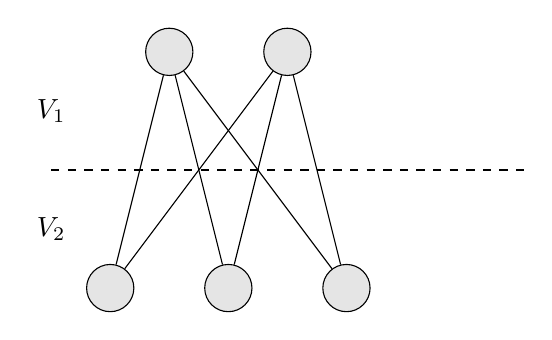
\begin{tikzpicture}[scale=1.5]
        % Nodes
        \node[circle, draw, fill=gray!20, minimum size=0.6cm] (1) at (0.5, 2) {};
        \node[circle, draw, fill=gray!20, minimum size=0.6cm] (2) at (1.5, 2) {};
        \node[circle, draw, fill=gray!20, minimum size=0.6cm] (3) at (0, 0) {};
        \node[circle, draw, fill=gray!20, minimum size=0.6cm] (4) at (1, 0) {};
        \node[circle, draw, fill=gray!20, minimum size=0.6cm] (5) at (2, 0) {};
        
        % Edges
        \draw[-] (1) -- (3);
        \draw[-] (1) -- (4);
        \draw[-] (1) -- (5);
        \draw[-] (2) -- (3);    
        \draw[-] (2) -- (4);
        \draw[-] (2) -- (5);


        % Labels
        \draw[dashed] (-0.5, 1) -- (3.5, 1);
        \node at (-0.5, 1.5) {$V_1$};
        \node at (-0.5, 0.5) {$V_2$};
    \end{tikzpicture}
    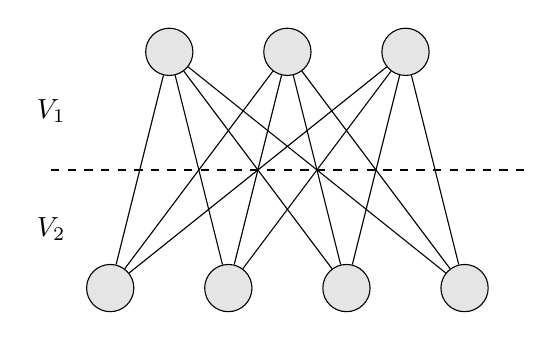
\begin{tikzpicture}[scale=1.5]
        % Nodes
        \node[circle, draw, fill=gray!20, minimum size=0.6cm] (1) at (0.5, 2) {};
        \node[circle, draw, fill=gray!20, minimum size=0.6cm] (2) at (1.5, 2) {};
        \node[circle, draw, fill=gray!20, minimum size=0.6cm] (3) at (2.5, 2) {};
        \node[circle, draw, fill=gray!20, minimum size=0.6cm] (4) at (0, 0) {};
        \node[circle, draw, fill=gray!20, minimum size=0.6cm] (5) at (1, 0) {};
        \node[circle, draw, fill=gray!20, minimum size=0.6cm] (6) at (2, 0) {};
        \node[circle, draw, fill=gray!20, minimum size=0.6cm] (7) at (3, 0) {};

        % Edges
        \draw[-] (1) -- (4);
        \draw[-] (1) -- (5);
        \draw[-] (1) -- (6);
        \draw[-] (2) -- (4);
        \draw[-] (2) -- (5);
        \draw[-] (2) -- (6);
        \draw[-] (3) -- (4);
        \draw[-] (3) -- (5);
        \draw[-] (3) -- (6);
        \draw[-] (3) -- (7);
        \draw[-] (2) -- (7);
        \draw[-] (1) -- (7);

        % Labels
        \draw[dashed] (-0.5, 1) -- (3.5, 1);
        \node at (-0.5, 1.5) {$V_1$};
        \node at (-0.5, 0.5) {$V_2$};
    \end{tikzpicture}
    \caption{Complete bipartite graphs $K_{2,2}$ and $K_{3,3}$.}
\end{figure}

\subsubsection{Matching}
A matching in a bipartite graph is a subset of edges such that no two edges share a common vertex.


        \begin{figure}[H]
    \centering
    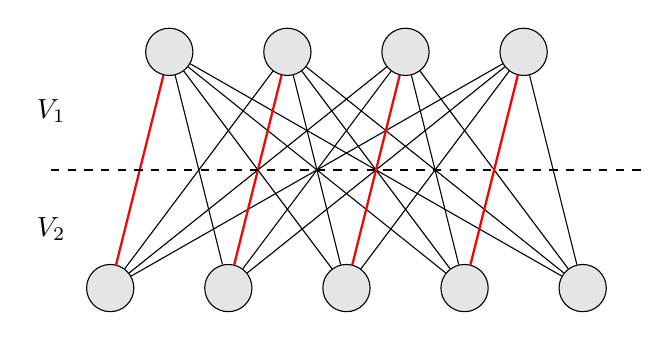
\begin{tikzpicture}[scale=1.5]
        % Nodes
        \node[circle, draw, fill=gray!20, minimum size=0.6cm] (1) at (0.5, 2) {};
        \node[circle, draw, fill=gray!20, minimum size=0.6cm] (2) at (1.5, 2) {};
        \node[circle, draw, fill=gray!20, minimum size=0.6cm] (3) at (2.5, 2) {};
        \node[circle, draw, fill=gray!20, minimum size=0.6cm] (4) at (3.5, 2) {};
        \node[circle, draw, fill=gray!20, minimum size=0.6cm] (5) at (0, 0) {};
        \node[circle, draw, fill=gray!20, minimum size=0.6cm] (6) at (1, 0) {};
        \node[circle, draw, fill=gray!20, minimum size=0.6cm] (7) at (2, 0) {};
        \node[circle, draw, fill=gray!20, minimum size=0.6cm] (8) at (3, 0) {};
        \node[circle, draw, fill=gray!20, minimum size=0.6cm] (9) at (4, 0) {};

        % Edges (Complete graph)
        \draw[-] (1) -- (5);
        \draw[-] (1) -- (6);
        \draw[-] (1) -- (7);
        \draw[-] (1) -- (8);
        \draw[-] (1) -- (9);
        \draw[-] (2) -- (5);
        \draw[-] (2) -- (6);
        \draw[-] (2) -- (7);
        \draw[-] (2) -- (8);
        \draw[-] (2) -- (9);
        \draw[-] (3) -- (5);
        \draw[-] (3) -- (6);
        \draw[-] (3) -- (7);
        \draw[-] (3) -- (8);
        \draw[-] (3) -- (9);
        \draw[-] (4) -- (5);
        \draw[-] (4) -- (6);
        \draw[-] (4) -- (7);
        \draw[-] (4) -- (8);
        \draw[-] (4) -- (9);

        % Matching (highlighted edges)
        \draw[thick, red] (1) -- (5);
        \draw[thick, red] (2) -- (6);
        \draw[thick, red] (3) -- (7);
        \draw[thick, red] (4) -- (8);

        \draw[dashed] (-0.5, 1) -- (4.5, 1);
        \node at (-0.5, 1.5) {$V_1$};
        \node at (-0.5, 0.5) {$V_2$};
    \end{tikzpicture}
    \caption{Complete bipartite graph with a matching highlighted in red.}
\end{figure}

The maximum matching is the matching with the maximum number of edges. The complete matching is the matching where all vertices in $V_1$ have an edge.

\section{Graph Operations}
\subsection{Subgraph}
A subgraph of a graph $G = (V,E)$ is a graph $G' = (V',E')$ such that $V' \subseteq V$ and $E' \subseteq E$. We call the subgraph proper if $V' \neq V$ and $E' \neq E$. 

\[
G = (V,E), \quad \text{Subgraph induced by } V' \subseteq V \text{ is } G' = (V',E'), \quad E' = \{(u,v) \in E \mid u,v \in V'\}
\]

\begin{figure}[H]
    \centering
    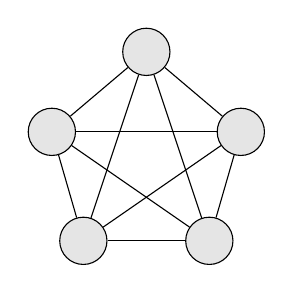
\begin{tikzpicture}[scale=0.8]
        % K_5 (Pentagon)
        \node[circle, draw, fill=gray!20, minimum size=0.6cm] (k5a) at (0, 0) {};
        \node[circle, draw, fill=gray!20, minimum size=0.6cm] (k5b) at (2, 0) {};
        \node[circle, draw, fill=gray!20, minimum size=0.6cm] (k5c) at (2.5, 1.73) {};
        \node[circle, draw, fill=gray!20, minimum size=0.6cm] (k5d) at (1, 3) {};
        \node[circle, draw, fill=gray!20, minimum size=0.6cm] (k5e) at (-0.5, 1.73) {};
        \draw[-] (k5a) -- (k5b);
        \draw[-] (k5b) -- (k5c);
        \draw[-] (k5c) -- (k5d);
        \draw[-] (k5d) -- (k5e);
        \draw[-] (k5e) -- (k5a);
        \draw[-] (k5a) -- (k5c);
        \draw[-] (k5a) -- (k5d);
        \draw[-] (k5b) -- (k5d);
        \draw[-] (k5b) -- (k5e);
        \draw[-] (k5c) -- (k5e);
    \end{tikzpicture}
    \hspace{1cm}
    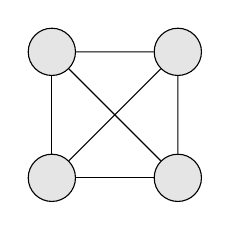
\begin{tikzpicture}[scale=0.8]
        % Induced graph (Triangle)
        \node[circle, draw, fill=gray!20, minimum size=0.6cm] (i1) at (0, 0) {};
        \node[circle, draw, fill=gray!20, minimum size=0.6cm] (i2) at (2, 0) {};
        \node[circle, draw, fill=gray!20, minimum size=0.6cm] (i3) at (0, 2) {};
        \node[circle, draw, fill=gray!20, minimum size=0.6cm] (i4) at (2, 2) {};
        \draw[-] (i1) -- (i2);
        \draw[-] (i1) -- (i3);
        \draw[-] (i2) -- (i3);
        \draw[-] (i1) -- (i4);
        \draw[-] (i2) -- (i4);
        \draw[-] (i3) -- (i4);
    \end{tikzpicture}
    \caption{Complete graph $K_5$ and its induced graph.}
    \label{fig:K5_induced}
\end{figure}

\subsection{Other operations}
\begin{enumerate}
    \item \textbf{Remaining a single edge: } $G = (V,E) \implies G' = (V,E')$, where $E' = E - \{e\}$, $e \in E$.
    \item \textbf{Adding an edge: } $G = (V,E) \implies G' = (V,E')$, where $E' = E \cup \{e\}$, $e \notin E$. This is not a subgraph.
    
    Some operations can be done for more than one edge:
    \[
    (V,E) \implies (V,E') \text{ where } E' = E - \{e_1, e_2, \ldots, e_k\} \text{ or } E' = E \cup \{e_1, e_2, \ldots, e_k\}
    \]

    \item \textbf{Edge contractions: } removing an edge $e = (u,v)$ and merging the vertices $u$ and $v$ into a single vertex $w$. The new graph is denoted as $G' = (V',E')$, where $V' = V - \{u,v\} \cup \{w\}$ and $E'$ contains all edges from $E$ except for those incident to $u$ and $v$.
    \begin{center}
        \begin{figure}[H]
            \centering
            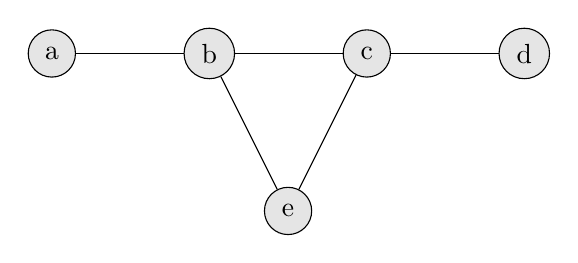
\begin{tikzpicture}
                % Original graph
                \node[circle, draw, fill=gray!20, minimum size=0.6cm] (u) at (0, 0) {a};
                \node[circle, draw, fill=gray!20, minimum size=0.6cm] (v) at (2, 0) {b};
                \node[circle, draw, fill=gray!20, minimum size=0.6cm] (w) at (4, 0) {c};
                \node[circle, draw, fill=gray!20, minimum size=0.6cm] (x) at (6, 0) {d};
                \node[circle, draw, fill=gray!20, minimum size=0.6cm] (y) at (3, -2) {e};

                \draw[-] (u) -- (v);
                \draw[-] (v) -- (w);
                \draw[-] (w) -- (x);
                \draw[-] (v) -- (y);
                \draw[-] (w) -- (y);
            \end{tikzpicture}
            \hspace{1cm}
            % Contracted graph
            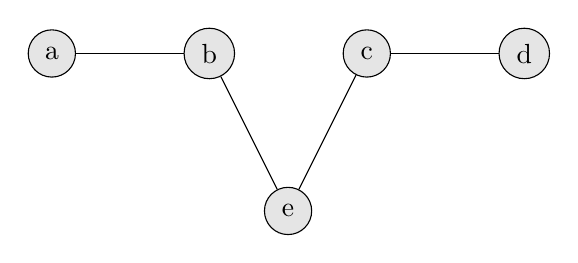
\begin{tikzpicture}
                % Contracted graph
                \node[circle, draw, fill=gray!20, minimum size=0.6cm] (u) at (0, 0) {a};
                \node[circle, draw, fill=gray!20, minimum size=0.6cm] (v) at (2, 0) {b};
                \node[circle, draw, fill=gray!20, minimum size=0.6cm] (w) at (4, 0) {c};
                \node[circle, draw, fill=gray!20, minimum size=0.6cm] (x) at (6, 0) {d};
                \node[circle, draw, fill=gray!20, minimum size=0.6cm] (y) at (3, -2) {e};

                \draw[-] (u) -- (v);
                \draw[-] (w) -- (x);
                \draw[-] (v) -- (y);
                \draw[-] (w) -- (y);
            \end{tikzpicture}
            \end{figure}
            \begin{figure}[H]
            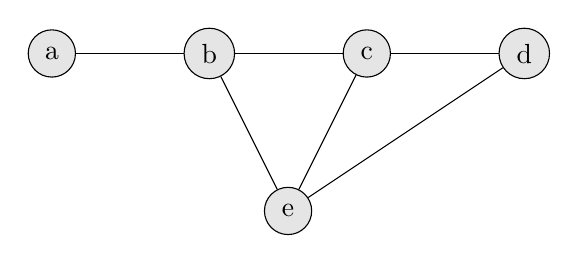
\begin{tikzpicture}
                \node[circle, draw, fill=gray!20, minimum size=0.6cm] (u) at (0, 0) {a};
                \node[circle, draw, fill=gray!20, minimum size=0.6cm] (v) at (2, 0) {b};
                \node[circle, draw, fill=gray!20, minimum size=0.6cm] (w) at (4, 0) {c};
                \node[circle, draw, fill=gray!20, minimum size=0.6cm] (x) at (6, 0) {d};
                \node[circle, draw, fill=gray!20, minimum size=0.6cm] (y) at (3, -2) {e};

                \draw[-] (u) -- (v);
                \draw[-] (v) -- (w);
                \draw[-] (w) -- (x);
                \draw[-] (v) -- (y);
                \draw[-] (w) -- (y);
                \draw[-] (x) -- (y);
            \end{tikzpicture}
            \hspace{1cm}
            % Contracted graph with new edge
            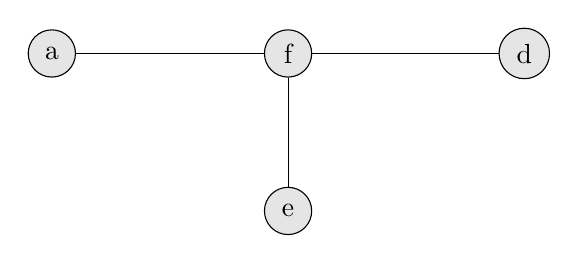
\begin{tikzpicture}
                % Contracted graph with new edge
                \node[circle, draw, fill=gray!20, minimum size=0.6cm] (u) at (0, 0) {a};
                \node[circle, draw, fill=gray!20, minimum size=0.6cm] (v) at (3, 0) {f};
                \node[circle, draw, fill=gray!20, minimum size=0.6cm] (x) at (6, 0) {d};
                \node[circle, draw, fill=gray!20, minimum size=0.6cm] (y) at (3, -2) {e};

                \draw[-] (u) -- (v);
                \draw[-] (v) -- (x);
                \draw[-] (v) -- (y);
            \end{tikzpicture}
            \caption{Operations on a graph: edge contraction and adding and removing edges.}
            \label{fig:edge_contraction}
        \end{figure}
    \end{center}
\end{enumerate}

\subsection{Graph representation}
\begin{enumerate}
    \item \textbf{Incidence list:} List vertices and for each vertex, list the edges incident to it.
    \begin{figure}[H]
        \centering
        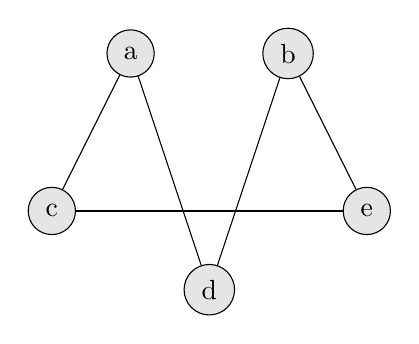
\begin{tikzpicture}
            % Nodes
            \node[circle, draw, fill=gray!20, minimum size=0.6cm] (1) at (0, 0) {a};
            \node[circle, draw, fill=gray!20, minimum size=0.6cm] (2) at (2, 0) {b};
            \node[circle, draw, fill=gray!20, minimum size=0.6cm] (3) at (-1, -2) {c};
            \node[circle, draw, fill=gray!20, minimum size=0.6cm] (4) at (1, -3) {d};
            \node[circle, draw, fill=gray!20, minimum size=0.6cm] (5) at (3, -2) {e};

            % Edges
            \draw[-] (1) -- (3);
            \draw[-] (1) -- (4);
            \draw[-] (3) -- (5);
            \draw[-] (4) -- (2);
            \draw[-] (2) -- (5);
        \end{tikzpicture}
        \hspace{1cm}
        \begin{tabular}{c|c}
            Vertex & Neighbors \\
            \hline
            a & (c,d) \\
            b & (d,e) \\
            c & (a,e) \\
            d & (a,b) \\
            e & (b,c) \\
        \end{tabular}
        \caption{Graph representation using incidence list. Useful for sparse graphs.}
        \label{fig:incidence_list}
    \end{figure}
    This representation is also useful for directed graphs, where the edges are directed from one vertex to another:
    \begin{figure}[H]
        \centering
        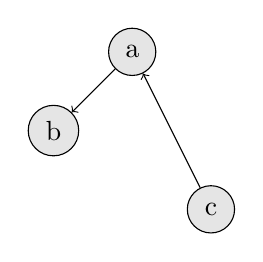
\begin{tikzpicture}
            % Nodes
            \node[circle, draw, fill=gray!20, minimum size=0.6cm] (1) at (0, 0) {a};
            \node[circle, draw, fill=gray!20, minimum size=0.6cm] (2) at (-1, -1) {b};
            \node[circle, draw, fill=gray!20, minimum size=0.6cm] (3) at (1, -2) {c};
            % Edges
            \draw[->] (3) -- (1);
            \draw[->] (1) -- (2);
        \end{tikzpicture}
        \hspace{1cm}
        \begin{tabular}{c|c}
            Initial Vertex & Terminal Vertex \\
            \hline
            a & b \\
            b & - \\
            c & a \\
        \end{tabular}
        \caption{Directed graph representation using incidence list.}
        \label{fig:directed_incidence_list}
    \end{figure}
    \item \textbf{Adjacency matrix:} A square matrix where the element at row $i$ and column $j$ indicates whether there is an edge between vertex $i$ and vertex $j$.
    \[
    (A)_{ij} = \begin{cases}
        1 & \text{if there is an edge between } i \text{ and } j \\
        0 & \text{otherwise}
    \end{cases}
    \]
    \begin{figure}[H]
        \centering
        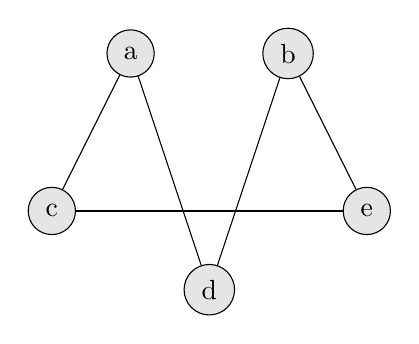
\begin{tikzpicture}
            % Nodes
            \node[circle, draw, fill=gray!20, minimum size=0.6cm] (1) at (0, 0) {a};
            \node[circle, draw, fill=gray!20, minimum size=0.6cm] (2) at (2, 0) {b};
            \node[circle, draw, fill=gray!20, minimum size=0.6cm] (3) at (-1, -2) {c};
            \node[circle, draw, fill=gray!20, minimum size=0.6cm] (4) at (1, -3) {d};
            \node[circle, draw, fill=gray!20, minimum size=0.6cm] (5) at (3, -2) {e};

            % Edges
            \draw[-] (1) -- (3);
            \draw[-] (1) -- (4);
            \draw[-] (3) -- (5);
            \draw[-] (4) -- (2);
            \draw[-] (2) -- (5);
        \end{tikzpicture}
        \hspace{1cm}
        \renewcommand{\arraystretch}{1} % Adjust this value as needed
        $A = \begin{pmatrix}
            0 & 1 & 1 & 0 & 0 \\
            0 & 0 & 0 & 1 & 1 \\
            1 & 0 & 0 & 0 & 1 \\
            1 & 1 & 0 & 0 & 0 \\
            0 & 1 & 1 & 0 & 0 \\
        \end{pmatrix}$
        \caption{Graph representation using adjacency matrix. Useful for dense graphs.}
        \label{fig:adjacency_matrix}
    \end{figure}

    For directed graphs, the adjacency matrix is not symmetric. The element at row $i$ and column $j$ indicates whether there is a directed edge \textbf{from} vertex $i$ to vertex $j$.
    \begin{figure}[H]
        \centering
        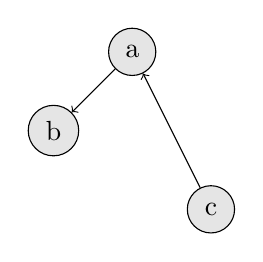
\begin{tikzpicture}
            % Nodes
            \node[circle, draw, fill=gray!20, minimum size=0.6cm] (1) at (0, 0) {a};
            \node[circle, draw, fill=gray!20, minimum size=0.6cm] (2) at (-1, -1) {b};
            \node[circle, draw, fill=gray!20, minimum size=0.6cm] (3) at (1, -2) {c};
            % Edges
            \draw[->] (3) -- (1);
            \draw[->] (1) -- (2);
        \end{tikzpicture}
        \hspace{1cm}
        \renewcommand{\arraystretch}{1} % Adjust this value as needed
        $A = \begin{pmatrix}
            0 & 1 & 0 \\
            0 & 0 & 0 \\
            1 & 0 & 0 \\
        \end{pmatrix}$
        \caption{Directed graph representation using adjacency matrix.}
        \label{fig:directed_adjacency_matrix}
    \end{figure}

    For multigraphs, the adjacency matrix can be modified to account for multiple edges between vertices. The element at row $i$ and column $j$ indicates the number of edges between vertex $i$ and vertex $j$.

    \item \textbf{Incidence matrix:} A matrix where the rows represent edges and the columns represent vertices. The element at row $i$ and column $j$ indicates whether edge $i$ is incident to vertex $j$. For undirected graphs, the element is 1 if the edge is incident to the vertex, and 0 otherwise. For directed graphs, the element is 1 if the edge is directed towards the vertex, -1 if it is directed away from the vertex, and 0 otherwise.
    \begin{figure}[H]
        \centering
        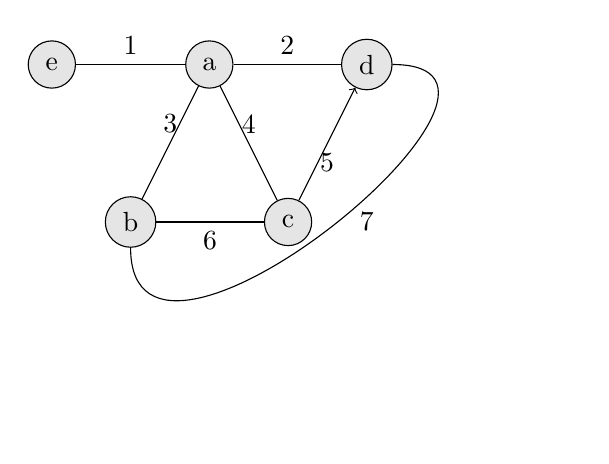
\begin{tikzpicture}
            % Nodes
            \node[circle, draw, fill=gray!20, minimum size=0.6cm] (1) at (0, 0) {a};
            \node[circle, draw, fill=gray!20, minimum size=0.6cm] (2) at (-1, -2) {b};
            \node[circle, draw, fill=gray!20, minimum size=0.6cm] (3) at (1, -2) {c};
            \node[circle, draw, fill=gray!20, minimum size=0.6cm] (4) at (2, 0) {d};
            \node[circle, draw, fill=gray!20, minimum size=0.6cm] (5) at (-2, 0) {e};

            % Edges
            \draw[-] (1) -- (3) node[midway, above] {4};
            \draw[-] (1) -- (4) node[midway, above] {2};
            \draw[-] (1) -- (5) node[midway, above] {1};
            \draw[-] (1) -- (2) node[midway, above] {3};
            \draw[-, in = 270, out = 0, looseness = 1.5] (4) to (2); 
            \node at (2, -2) {7};
            \draw[-] (2) -- (3) node[midway, below] {6};
            \draw[->] (3) -- (4) node[midway, below] {5};

        \end{tikzpicture}
        \hspace{0.5cm}
        \renewcommand{\arraystretch}{1} % Adjust this value as needed
        $I = \begin{pmatrix}
            1 & 1 & 1 & 1 & 0 & 0 & 0 \\
            0 & 0 & 1 & 0 & 0 & 1 & 1 \\
            0 & 0 & 0 & 1 & -1 & 1 & 0 \\
            0 & 1 & 0 & 0 & 1 & 0 & 1 \\
            1 & 0 & 0 & 0 & 0 & 0 & 1 \\
            \end{pmatrix}$
        \caption{Graph representation using incidence matrix.}
        \label{fig:incidence_matrix}
    \end{figure}
\end{enumerate}

\subsection{Graph isomorphism}
Two graphs $G_1 = (V_1,E_1)$ and $G_2 = (V_2,E_2)$ are isomorphic if there exists a bijection $f: V_1 \to V_2$ such that $(u,v) \in E_1 \iff (f(u),f(v)) \in E_2$. This means that the two graphs have the same structure, even if their representations are different. Then, $f$ is called an isomorphism.
\begin{figure}[H]
    \centering
    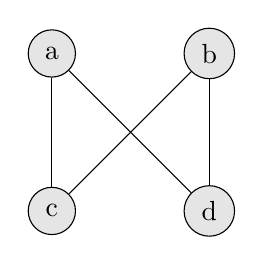
\begin{tikzpicture}
        % Graph 1
        \node[circle, draw, fill=gray!20, minimum size=0.6cm] (1) at (0, 0) {a};
        \node[circle, draw, fill=gray!20, minimum size=0.6cm] (2) at (2, 0) {b};
        \node[circle, draw, fill=gray!20, minimum size=0.6cm] (3) at (0, -2) {c};
        \node[circle, draw, fill=gray!20, minimum size=0.6cm] (4) at (2, -2) {d};

        \draw[-] (1) -- (3);
        \draw[-] (1) -- (4);
        \draw[-] (2) -- (3);
        \draw[-] (2) -- (4);

    \end{tikzpicture}
    \hspace{1cm}
    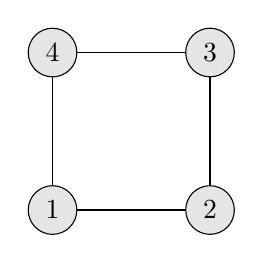
\begin{tikzpicture}
        % Graph 2
        \node[circle, draw, fill=gray!20, minimum size=0.6cm] (1) at (0, 0) {4};
        \node[circle, draw, fill=gray!20, minimum size=0.6cm] (2) at (2, 0) {3};
        \node[circle, draw, fill=gray!20, minimum size=0.6cm] (4) at (0, -2) {1};
        \node[circle, draw, fill=gray!20, minimum size=0.6cm] (3) at (2, -2) {2};

        \draw[-] (1) -- (2);
        \draw[-] (2) -- (3);
        \draw[-] (3) -- (4);
        \draw[-] (4) -- (1);
    \end{tikzpicture}
    \caption{Two isomorphic graphs.}
    \label{fig:isomorphic_graphs}
\end{figure}

The isomorphism can be represented as a mapping between the vertices of the two graphs. For example, in the above graphs, we can have the following mapping:
\begin{align*}
    a & \mapsto 1 \\
    b & \mapsto 3 \\
    c & \mapsto 4 \\
    d & \mapsto 2 \\
\end{align*}

\subsection{Graph invariants}
A graph invariant is a property of a graph that remains unchanged under isomorphism. Some common graph invariants include:
\begin{itemize}
    \item Number of vertices and edges
    \item Degree sequence (the list of degrees of the vertices)
\end{itemize}

\begin{figure}[H]
    \centering
    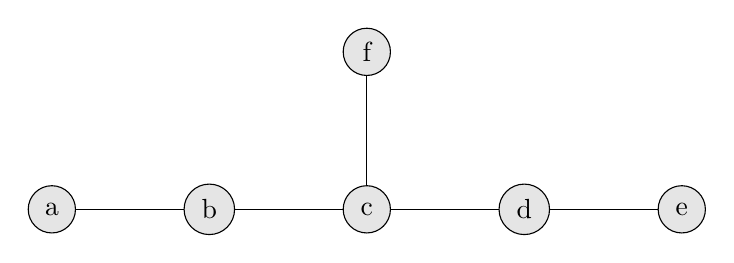
\begin{tikzpicture}
        % Graph 1
        \node[circle, draw, fill=gray!20, minimum size=0.6cm] (1) at (0, 0) {a};
        \node[circle, draw, fill=gray!20, minimum size=0.6cm] (2) at (2, 0) {b};
        \node[circle, draw, fill=gray!20, minimum size=0.6cm] (3) at (4, 0) {c};
        \node[circle, draw, fill=gray!20, minimum size=0.6cm] (4) at (6, 0) {d};
        \node[circle, draw, fill=gray!20, minimum size=0.6cm] (5) at (8, 0) {e};
        \node[circle, draw, fill=gray!20, minimum size=0.6cm] (6) at (4, 2) {f};

        \draw[-] (1) -- (2);
        \draw[-] (2) -- (3);
        \draw[-] (3) -- (4);
        \draw[-] (4) -- (5);
        \draw[-] (3) -- (6);

        \end{tikzpicture}
    \end{figure}
    \begin{figure}[H]
        \centering
        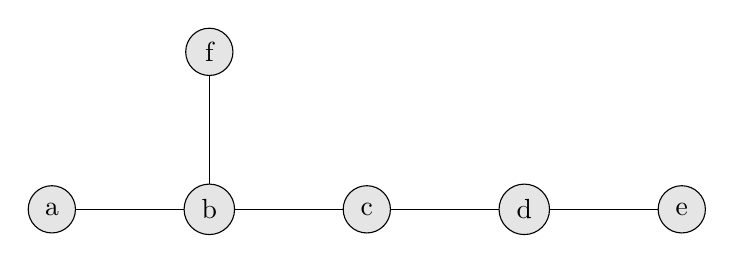
\begin{tikzpicture}
        % Graph 2
        \node[circle, draw, fill=gray!20, minimum size=0.6cm] (1) at (0, 0) {a};
        \node[circle, draw, fill=gray!20, minimum size=0.6cm] (2) at (2, 0) {b};
        \node[circle, draw, fill=gray!20, minimum size=0.6cm] (3) at (4, 0) {c};
        \node[circle, draw, fill=gray!20, minimum size=0.6cm] (4) at (6, 0) {d};
        \node[circle, draw, fill=gray!20, minimum size=0.6cm] (5) at (8, 0) {e};
        \node[circle, draw, fill=gray!20, minimum size=0.6cm] (6) at (2, 2) {f};

        \draw[-] (1) -- (2);
        \draw[-] (2) -- (3);
        \draw[-] (3) -- (4);
        \draw[-] (4) -- (5);
        \draw[-] (2) -- (6);

        \end{tikzpicture}
        \caption{Two non-isomorphic graphs with the same number of vertices and edges, but different degree sequences.}
        \label{fig:non_isomorphic_graphs}
\end{figure}

If we try to find an isomorphism between the two graphs in Figure \ref{fig:non_isomorphic_graphs}, we will find that the degree sequence of the vertices is different. For example, vertex $c$ has two neighbors of degree 2 and one neighbor of degree 1 on the left graph, while on the right graph, vertex $c$ has two neighbors of degree 1 and one neighbor of degree 2. This means that the two graphs are not isomorphic.

\begin{figure}[H]
    \centering
    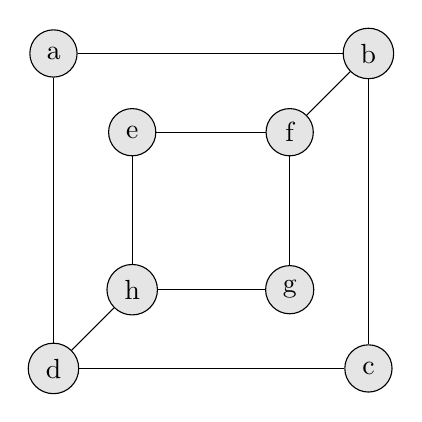
\begin{tikzpicture}
        % Graph 1
        \node[circle, draw, fill=gray!20, minimum size=0.6cm] (1) at (0, 0) {a};
        \node[circle, draw, fill=gray!20, minimum size=0.6cm] (2) at (4, 0) {b};
        \node[circle, draw, fill=gray!20, minimum size=0.6cm] (3) at (4, -4) {c};
        \node[circle, draw, fill=gray!20, minimum size=0.6cm] (4) at (0, -4) {d};
        \node[circle, draw, fill=gray!20, minimum size=0.6cm] (5) at (1, -1) {e};
        \node[circle, draw, fill=gray!20, minimum size=0.6cm] (6) at (3, -1) {f};
        \node[circle, draw, fill=gray!20, minimum size=0.6cm] (7) at (3, -3) {g};
        \node[circle, draw, fill=gray!20, minimum size=0.6cm] (8) at (1, -3) {h};

        \draw[-] (1) -- (2);
        \draw[-] (2) -- (3);
        \draw[-] (3) -- (4);
        \draw[-] (4) -- (1);
        \draw[-] (5) -- (6);
        \draw[-] (6) -- (7);
        \draw[-] (7) -- (8);
        \draw[-] (8) -- (5);
        \draw[-] (2) -- (6);
        \draw[-] (4) -- (8);
    \end{tikzpicture}
    \hspace{1cm}
    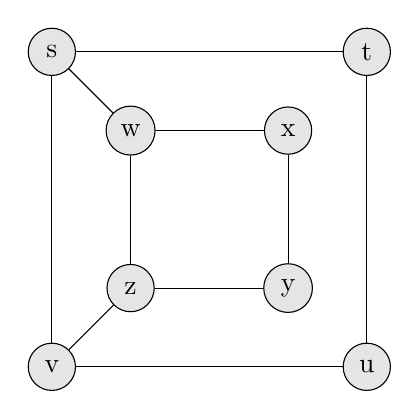
\begin{tikzpicture}
        % Graph 2
        \node[circle, draw, fill=gray!20, minimum size=0.6cm] (1) at (0, 0) {s};
        \node[circle, draw, fill=gray!20, minimum size=0.6cm] (2) at (4, 0) {t};
        \node[circle, draw, fill=gray!20, minimum size=0.6cm] (3) at (4, -4) {u};
        \node[circle, draw, fill=gray!20, minimum size=0.6cm] (4) at (0, -4) {v};
        \node[circle, draw, fill=gray!20, minimum size=0.6cm] (5) at (1, -1) {w};
        \node[circle, draw, fill=gray!20, minimum size=0.6cm] (6) at (3, -1) {x};
        \node[circle, draw, fill=gray!20, minimum size=0.6cm] (7) at (3, -3) {y};
        \node[circle, draw, fill=gray!20, minimum size=0.6cm] (8) at (1, -3) {z};

        \draw[-] (1) -- (2);
        \draw[-] (2) -- (3);
        \draw[-] (3) -- (4);
        \draw[-] (4) -- (1);
        \draw[-] (5) -- (6);
        \draw[-] (6) -- (7);
        \draw[-] (7) -- (8);
        \draw[-] (8) -- (5);
        \draw[-] (1) -- (5);
        \draw[-] (4) -- (8);
    \end{tikzpicture}
    \caption{Two non-isomorphic graphs.}
    \label{fig:isomorphic_graphs_2}
\end{figure}
In the above example, by listing the vertices and their neighbors, we can see that the two graphs don't have the same degree sequences:
\begin{align*}
    a & : 2 & \quad & s : 3 \\
    b & : 3 & \quad & t : 2 \\
    c & : 2 & \quad & u : 2 \\
    d & : 3 & \quad & v : 3 \\
    e & : 2 & \quad & w : 3 \\
    f & : 3 & \quad & x : 2 \\
    g & : 2 & \quad & y : 2 \\
    h & : 3 & \quad & z : 3 \\
\end{align*}

The degree sequences are different, so the two graphs are not isomorphic. We can also see that the two graphs have cycles of different lengths. The first graph has a cycle of length 4, while the second graph has a cycle of length 3. This is another indication that the two graphs are not isomorphic.

\subsection{Adjacency matrix and isomorphism}
Two graphs are isomorphic if their adjacency matrices can be transformed into each other by permuting the rows and columns. This means that the two graphs have the same structure, even if their representations are different.
\begin{figure}[H]
    \centering
    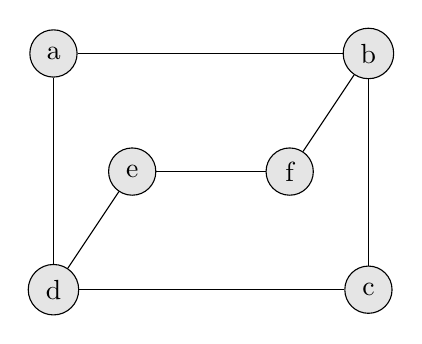
\begin{tikzpicture}
        % Graph 1
        \node[circle, draw, fill=gray!20, minimum size=0.6cm] (1) at (0, 0) {a};
        \node[circle, draw, fill=gray!20, minimum size=0.6cm] (2) at (4, 0) {b};
        \node[circle, draw, fill=gray!20, minimum size=0.6cm] (3) at (4, -3) {c};
        \node[circle, draw, fill=gray!20, minimum size=0.6cm] (4) at (0, -3) {d};
        \node[circle, draw, fill=gray!20, minimum size=0.6cm] (5) at (1, -1.5) {e};
        \node[circle, draw, fill=gray!20, minimum size=0.6cm] (6) at (3, -1.5) {f};

        \draw[-] (1) -- (2);
        \draw[-] (2) -- (3);
        \draw[-] (3) -- (4);
        \draw[-] (4) -- (1);
        \draw[-] (5) -- (6);
        \draw[-] (4) -- (5);
        \draw[-] (2) -- (6);
    \end{tikzpicture}
    \hspace{1cm}
    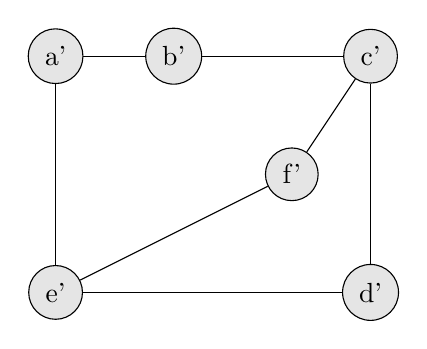
\begin{tikzpicture}
        % Graph 2
        \node[circle, draw, fill=gray!20, minimum size=0.6cm] (1) at (0, 0) {a'};
        \node[circle, draw, fill=gray!20, minimum size=0.6cm] (2) at (1.5, 0) {b'};
        \node[circle, draw, fill=gray!20, minimum size=0.6cm] (3) at (4, 0) {c'};
        \node[circle, draw, fill=gray!20, minimum size=0.6cm] (4) at (4, -3) {d'};
        \node[circle, draw, fill=gray!20, minimum size=0.6cm] (5) at (0, -3) {e'};
        \node[circle, draw, fill=gray!20, minimum size=0.6cm] (6) at (3, -1.5) {f'};

        \draw[-] (1) -- (2);
        \draw[-] (2) -- (3);
        \draw[-] (3) -- (4);
        \draw[-] (4) -- (5);
        \draw[-] (5) -- (1);
        \draw[-] (6) -- (5);
        \draw[-] (6) -- (3);
    \end{tikzpicture}
    \caption{Two isomorphic graphs.}
    \label{fig:isomorphic_graphs_3}
\end{figure}
The adjacency matrices of the two graphs are:
\renewcommand{\arraystretch}{1} % Adjust this value as needed

\begin{align*}
    A_1 &= \begin{pmatrix}
        0 & 1 & 0 & 1 & 0 & 0 \\
        1 & 0 & 1 & 0 & 0 & 1 \\
        0 & 1 & 0 & 1 & 0 & 0 \\
        1 & 0 & 1 & 0 & 1 & 0 \\
        0 & 0 & 0 & 1 & 0 & 1 \\
        0 & 1 & 0 & 0 & 1 & 0 \\
    \end{pmatrix} &
    A_2 &= \begin{pmatrix}
        1 & 0 & 0 & 0 & 1 & 0 \\
        1 & 0 & 1 & 0 & 0 & 0 \\
        0 & 1 & 0 & 1 & 0 & 1 \\
        0 & 0 & 1 & 0 & 1 & 0 \\
        1 & 0 & 0 & 1 & 0 & 1 \\
        0 & 0 & 1 & 0 & 1 & 0 \\
    \end{pmatrix}
\end{align*}

The adjacency matrices of the two graphs are not the same, but they can be transformed into each other by permuting the rows and columns. This means that the two graphs are isomorphic.
\[
A_2 = P A_1 P^T
\]
where $P$ is a permutation matrix that permutes the rows and columns of $A_1$ to obtain $A_2$.
\[
P = P_{16} P_{23} P_{34} P_{45} P_{51} P_{62}
\]
where $P_{ij}$ is the permutation matrix that swaps the $i$-th and $j$-th rows and columns of a matrix. The permutation matrix $P$ can be obtained by applying the following permutations to the rows and columns of $A_1$:
This means that the two graphs have the same structure, even if their representations are different.
   
\subsection{Paths}
A path in a graph is a sequence of vertices such that each vertex is connected to the next vertex by an edge. The length of a path is the number of edges in the path. A path is simple if it does not traverse any edge more than once.

\begin{figure}[H]
    \centering
    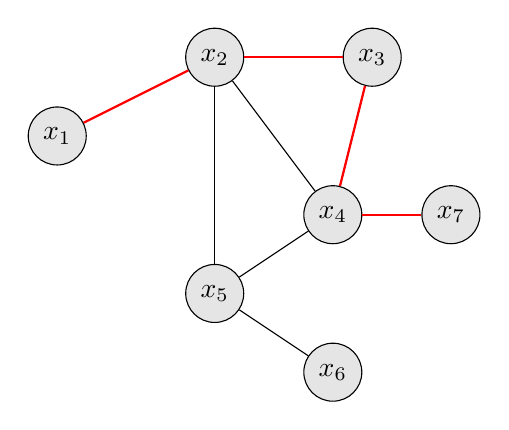
\begin{tikzpicture}
        % Nodes
        \node[circle, draw, fill=gray!20, minimum size=0.6cm] (1) at (0, 0) {$x_1$};
        \node[circle, draw, fill=gray!20, minimum size=0.6cm] (2) at (2, 1) {$x_2$};
        \node[circle, draw, fill=gray!20, minimum size=0.6cm] (3) at (4, 1) {$x_3$};
        \node[circle, draw, fill=gray!20, minimum size=0.6cm] (4) at (3.5, -1) {$x_4$};
        \node[circle, draw, fill=gray!20, minimum size=0.6cm] (5) at (2, -2) {$x_5$};
        \node[circle, draw, fill=gray!20, minimum size=0.6cm] (6) at (3.5, -3) {$x_6$};
        \node[circle, draw, fill=gray!20, minimum size=0.6cm] (7) at (5, -1) {$x_7$};


        % Edges
        \draw[-] (1) -- (2);
        \draw[-] (2) -- (3);
        \draw[-] (3) -- (4);
        \draw[-] (4) -- (5);
        \draw[-] (5) -- (6);
        \draw[-] (2) -- (4);
        \draw[-] (2) -- (5);

        % Highlighted path
        \draw[thick, red] (1) -- (2);
        \draw[thick, red] (2) -- (3);
        \draw[thick, red] (3) -- (4);
        \draw[thick, red] (4) -- (7);

    \end{tikzpicture}
    \caption{Graph with a marked path. The path is highlighted in red.}
    \label{fig:marked_path}
\end{figure}

In directed graphs, edges have to be be from beggining to end. 

\subsection{Connected graphs}
A graph is connected if there is a path between every pair of vertices. 

\paragraph{Theorem:} This path can be chosen simple.

\begin{figure}[H]
    \centering
    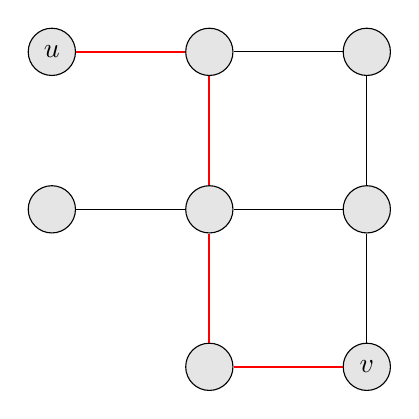
\begin{tikzpicture}
        % Nodes
        \node[circle, draw, fill=gray!20, minimum size=0.6cm] (1) at (0, 0) {$u$};
        \node[circle, draw, fill=gray!20, minimum size=0.6cm] (2) at (2, 0) {};
        \node[circle, draw, fill=gray!20, minimum size=0.6cm] (3) at (4, 0) {};
        \node[circle, draw, fill=gray!20, minimum size=0.6cm] (4) at (0,-2) {};
        \node[circle, draw, fill=gray!20, minimum size=0.6cm] (5) at (2,-2) {};
        \node[circle, draw, fill=gray!20, minimum size=0.6cm] (6) at (4,-2) {};
        \node[circle, draw, fill=gray!20, minimum size=0.6cm] (7) at (2,-4) {}; 
        \node[circle, draw, fill=gray!20, minimum size=0.6cm] (8) at (4,-4) {$v$};  


        % Edges
        \draw[-, thick, red] (1) -- (2);
        \draw[-, thick, red] (2) -- (5);
        \draw[-, thick, red] (5) -- (7);
        \draw[-, thick, red] (7) -- (8);
        \draw[-] (6) -- (5);
        \draw[-] (2) -- (3);
        \draw[-] (3) -- (6);
        \draw[-] (4) -- (5);
        \draw[-] (6) -- (8);

    \end{tikzpicture}
    \caption{Graph with a marked path. The path is highlighted in red.}
    \label{fig:marked_path_connected}
\end{figure}

\subsubsection{Connected components}
A connected component of a graph is any connected subgraph that is not a proper subgraph of any other connected subgraph. In other words, a connected component is a "piece" in which you can break a graph. A graph can have multiple connected components.

\subsubsection{Vertex and Edge cuts}
In a connected graph, a vertex or an edge is a cut if removing it disconnects the graph. 

\begin{figure}[H]
    \centering
    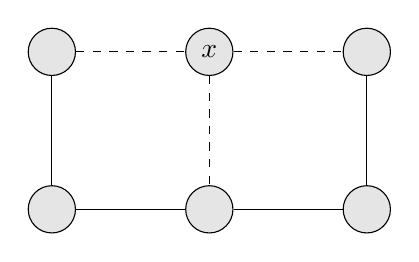
\begin{tikzpicture}
        % Nodes
        \node[circle, draw, fill=gray!20, minimum size=0.6cm] (1) at (0, 0) {};
        \node[circle, draw, fill=gray!20, minimum size=0.6cm] (2) at (2, 0) {$x$};
        \node[circle, draw, fill=gray!20, minimum size=0.6cm] (3) at (4, 0) {};
        \node[circle, draw, fill=gray!20, minimum size=0.6cm] (4) at (0,-2) {};
        \node[circle, draw, fill=gray!20, minimum size=0.6cm] (5) at (2,-2) {};
        \node[circle, draw, fill=gray!20, minimum size=0.6cm] (6) at (4,-2) {};


        % Edges
        \draw[dashed] (1) -- (2);
        \draw[dashed] (2) -- (3);
        \draw[dashed] (2) -- (5);
        \draw[-] (3) -- (6);
        \draw[-] (1) -- (4);
        \draw[-] (4) -- (5);
        \draw[-] (5) -- (6);

    \end{tikzpicture}
    \hspace{1cm}
    \begin{tikzpicture}
        % Nodes
        \node[circle, draw, fill=gray!20, minimum size=0.6cm] (1) at (0, 0) {};
        \node[circle, draw, fill=gray!20, minimum size=0.6cm] (2) at (2, -1) {$x$};
        \node[circle, draw, fill=gray!20, minimum size=0.6cm] (3) at (4, 0) {};
        \node[circle, draw, fill=gray!20, minimum size=0.6cm] (4) at (0,-2) {};
        \node[circle, draw, fill=gray!20, minimum size=0.6cm] (5) at (4,-2) {};


        % Edges
        \draw[-] (1) -- (4);
        \draw[-] (3) -- (5);
        \draw[dashed] (1) -- (2);
        \draw[dashed] (2) -- (3);
        \draw[dashed] (2) -- (5);
        \draw[dashed] (4) -- (2);
        \end{tikzpicture}
    \caption{Graphs showing a vertex cut. The vertex $x$ is not a cut vertex in the first graph, as removing it does not disconnect the graph. In the second graph, removing $x$ disconnects the graph.}
    \label{fig:marked_cut}
\end{figure}

\subsubsection{Vertex and Edge connectivity}
The vertex $\kappa (G)$ or edge $\lambda (G)$ connectivity of a graph is the minimum number of vertices or edges that need to be removed to disconnect the graph. 
\[
\kappa (G) \leq \lambda (G)
\]

For the connected graph in Figure \ref{fig:marked_cut}, the vertex connectivity is 2, as removing the vertex $x$ is not enough to disconnect the graph. The edge connectivity is 2, as removing any single edge does not disconnect the graph. For the second graph, the vertex connectivity is 1, as removing the vertex $x$ disconnects the graph. The edge connectivity is 2 as well, as removing any one edge does not disconnect the graph.
\[
\kappa (G_1) = 2 \quad \lambda (G_1) = 2 \quad \kappa (G_2) = 1 \quad \lambda (G_2) = 2
\]

For the complete graph $K_n$, the vertex and edge connectivity are both $n-1$.
\[
\kappa (K_n) = n-1 \quad \lambda (K_n) = n-1
\]

\paragraph{Theorem:} Let $G = (V,E)$ be a connected graph. Then, $|V| = n \implies |E| \leq n-1$.
If $|E| < n-1$, then $G$ can not be connected.

\subsection*{Example}
Provide an example of:
\begin{itemize}
    \item A regular bipartite graph.
    \item A regular graph of degree 3 with 9 vertices.
    \item A graph with $n$ vertices and $\dfrac{(n-1)(n-2)}{2}$ edges.
    \item A graph which is isomorphic to its complement.
\end{itemize}

\textbf{Note: } A regular graph is a graph where every vertex has the same degree.

\textbf{Note: } Given a graph $G$, the complement of $G$ is a graph $\bar{G}$ with the same vertices as $G$, but with edges that are not in $G$. In other words, if $(u,v) \in E(G)$, then $(u,v) \notin E(\bar{G})$ and vice versa.

\begin{figure}[H]
    \centering
    \begin{tikzpicture}
        % Nodes
        \node[circle, draw, fill=gray!20, minimum size=0.6cm] (1) at (0, 0) {a};
        \node[circle, draw, fill=gray!20, minimum size=0.6cm] (2) at (2, 0) {b};
        \node[circle, draw, fill=gray!20, minimum size=0.6cm] (3) at (4, 0) {c};
        \node[circle, draw, fill=gray!20, minimum size=0.6cm] (4) at (0, -2) {d};
        \node[circle, draw, fill=gray!20, minimum size=0.6cm] (5) at (2, -2) {e};
        \node[circle, draw, fill=gray!20, minimum size=0.6cm] (6) at (4, -2) {f};

        % Edges
        \draw[-] (1) -- (4);
        \draw[-] (2) -- (4);
        \draw[-] (3) -- (4);
        \draw[-] (1) -- (5);
        \draw[-] (2) -- (5);
        \draw[-] (3) -- (5);
        \draw[-] (1) -- (6);
        \draw[-] (2) -- (6);
        \draw[-] (3) -- (6);

    \end{tikzpicture}
    \hspace{1cm}
    \begin{tikzpicture}
        % Nodes
        \node[circle, draw, fill=gray!20, minimum size=0.6cm] (1) at (0, 0) {a};
        \node[circle, draw, fill=gray!20, minimum size=0.6cm] (2) at (2, 1) {b};
        \node[circle, draw, fill=gray!20, minimum size=0.6cm] (3) at (4, 0) {c};
        \node[circle, draw, fill=gray!20, minimum size=0.6cm] (4) at (0, -2) {d};
        \node[circle, draw, fill=gray!20, minimum size=0.6cm] (5) at (2, -2) {e};
        \node[circle, draw, fill=gray!20, minimum size=0.6cm] (6) at (4, -2) {f};
        \node[circle, draw, fill=gray!20, minimum size=0.6cm] (7) at (1, -1) {g};
        \node[circle, draw, fill=gray!20, minimum size=0.6cm] (8) at (3, -1) {h};
        \node[circle, draw, fill=gray!20, minimum size=0.6cm] (9) at (2, -3) {i};

        % Edges
        \draw[-] (1) -- (2);
        \draw[-] (2) -- (3);
        \draw[-] (1) -- (4);
        \draw[-] (1) -- (7);
        \draw[-] (3) -- (8);    
        \draw[-] (3) -- (6);
        \draw[-] (1) -- (7);
        \draw[-] (2) -- (7);
        \draw[-] (4) -- (5);
        \draw[-] (5) -- (8);
        \draw[-] (6) -- (8);
        \draw[-] (4) -- (9);
        \draw[-] (5) -- (9);
        \draw[-] (6) -- (9);
        \draw[-] (7) -- (8);

    \end{tikzpicture}
    \caption{A regular bipartite graph and an attempt of a regular graph of degree 3 with 9 vertices. The second graph is not regular, as the vertex $h$ has degree 4. It is not possible to create a regular graph of degree 3 with 9 vertices.}
    \label{fig:regular_bipartite_graph}
\end{figure}

\begin{figure}[H]
    \centering
    \begin{tikzpicture}
        % Nodes
        \node[circle, draw, fill=gray!20, minimum size=0.6cm] (1) at (0, 0) {a};
        \node[circle, draw, fill=gray!20, minimum size=0.6cm] (2) at (2, 0) {b};
        \node[circle, draw, fill=gray!20, minimum size=0.6cm] (3) at (4, 0) {c};
        \node[circle, draw, fill=gray!20, minimum size=0.6cm] (4) at (0,-2) {d};
        \node[circle, draw, fill=gray!20, minimum size=0.6cm] (5) at (2,-2) {e};
        \node[circle, draw, fill=gray!20, minimum size=0.6cm] (6) at (4,-2) {f};

        % Edges
        \draw[-] (1) -- (2);
        \draw[-] (2) -- (3);
        \draw[-] (3) -- (4);
        \draw[-] (4) -- (5);
        \draw[-] (5) -- (6);
        \draw[-] (1) -- (4);
        \draw[-] (1) -- (5);
        \draw[-] (1) -- (6);
        \draw[-] (3) -- (6);
        \draw[-] (3) -- (5);

    \end{tikzpicture}
    \hspace{1cm}
    \begin{tikzpicture}
        % Nodes
        \node[circle, draw, fill=gray!20, minimum size=0.6cm] (1) at (0, 0) {a};
        \node[circle, draw, fill=gray!20, minimum size=0.6cm] (2) at (2, 0) {b};
        \node[circle, draw, fill=gray!20, minimum size=0.6cm] (3) at (0,-2) {c};
        \node[circle, draw, fill=gray!20, minimum size=0.6cm] (4) at (2,-2) {d};

        % Edges
        \draw[-] (1) -- (2);
        \draw[-] (3) -- (4);
        \draw[-] (1) -- (3);

        \end{tikzpicture}
    \caption{A graph with $n = 6$ vertices and $\dfrac{(n-1)(n-2)}{2} = 10$ edges and a graph which is isomorphic to its complement.}
    \label{fig:complete_graph}
\end{figure}

\subsection*{Example}
Calculate the number of vertices of:
\begin{itemize}
    \item A regular graph of degree 2 with 9 edges.
    \item A regular graph with 6 edges.
    \item A graph with 10 edges, 2 vertices of degree 4 and the rest of degree 3.
\end{itemize}

By the handshaking lemma, we know that the sum of the degrees of all vertices is equal to twice the number of edges. This means that if we have a graph with $n$ vertices then:
\[
\sum_{i=1}^{n} d(v_i) = 2 |E| 
\]
where $d(v_i)$ is the degree of vertex $i$.

So we can establish the following equation for a regular graph of degree $d$:
\[
|V| = \frac{2 |E|}{d}
\]

For the first case, we have:
\[
|V| = \frac{9 \cdot 2}{2} = 9
\]

For the second case, we have:
\[
|V| = \frac{6 \cdot 2}{d} \implies d = 3 \text{ or } 2 \implies |V| = 4 \text{ or } 3
\]

For the third case, we have:
\[
20 = 2 \cdot 4 + (n-2) \cdot 3 \implies 20 = 8 + 3n - 6 \implies n = 6  
\]

\subsection*{Example}
Prove that the number of nodes of a self-complementary graph is either $4k$ or $4k + 1$ for some integer $k$.

\textbf{Proof:} Let $G$ be a self-complementary graph with $n$ vertices. Then, the number of edges in $G$ is equal to the number of edges in its complement $\bar{G}$. This means that:
\[
|E| + |\bar{E}| = \binom{n}{2} \implies 2 |E| = \binom{n}{2} \implies |E| = \frac{n(n-1)}{4}
\]

If $n$ is even, then $n(n-1)$ is divisible by 4. If $n$ is odd, then $n(n-1)$ is divisible by 2, but not by 4. This means that $n$ must be of the form $4k$ or $4k + 1$ for some integer $k$.

\subsection*{Example}
Conclude wether the following graphs are isomorphic or not:
\begin{figure}[H]
    \centering
    \begin{tikzpicture}
        % Graph 1
        \node[circle, draw, fill=gray!20, minimum size=0.6cm] (1) at (0, 0) {a};
        \node[circle, draw, fill=gray!20, minimum size=0.6cm] (2) at (-1, -2) {b};
        \node[circle, draw, fill=gray!20, minimum size=0.6cm] (5) at (1, -2) {e};
        \node[circle, draw, fill=gray!20, minimum size=0.6cm] (3) at (-2, -4) {c};
        \node[circle, draw, fill=gray!20, minimum size=0.6cm] (4) at (-0.5, -4) {d};
        \node[circle, draw, fill=gray!20, minimum size=0.6cm] (6) at (0.5, -4) {f};
        \node[circle, draw, fill=gray!20, minimum size=0.6cm] (7) at (2, -4) {g};

        \draw[-] (1) -- (2);
        \draw[-] (2) -- (3);
        \draw[-] (2) -- (4);
        \draw[-] (3) -- (4);
        \draw[-] (1) -- (5);
        \draw[-] (6) -- (5);
        \draw[-] (5) -- (7);

        \end{tikzpicture}
    \hspace{1cm}
    \begin{tikzpicture}
        \node[circle, draw, fill=gray!20, minimum size=0.6cm] (1) at (0, 0) {p};
        \node[circle, draw, fill=gray!20, minimum size=0.6cm] (2) at (0, -1) {q};
        \node[circle, draw, fill=gray!20, minimum size=0.6cm] (3) at (-1, -2) {r};
        \node[circle, draw, fill=gray!20, minimum size=0.6cm] (4) at (1, -2) {s};
        \node[circle, draw, fill=gray!20, minimum size=0.6cm] (5) at (0, -3) {t};
        \node[circle, draw, fill=gray!20, minimum size=0.6cm] (6) at (-1, -4) {u};
        \node[circle, draw, fill=gray!20, minimum size=0.6cm] (7) at (1, -4) {v};

        \draw[-] (1) -- (2);
        \draw[-] (2) -- (3);    
        \draw[-] (2) -- (4);
        \draw[-] (2) -- (5);
        \draw[-] (5) -- (6);
        \draw[-] (5) -- (7);
        \draw[-] (7) -- (6);
    \end{tikzpicture}
    \caption{Two graphs.}
    \label{fig:isomorphic_graphs_1}
\end{figure}

The two graphs are not isomorphic. We can see this by looking at the degree sequences of the vertices in each graph and realising that they are different.

If we consider the following graph:

\begin{figure}[H]
    \centering
    \begin{tikzpicture}
        % Graph 1
        \node[circle, draw, fill=gray!20, minimum size=0.6cm] (1) at (0, 0) {p};
        \node[circle, draw, fill=gray!20, minimum size=0.6cm] (2) at (-2, -1) {q};
        \node[circle, draw, fill=gray!20, minimum size=0.6cm] (3) at (-3, -2) {r};
        \node[circle, draw, fill=gray!20, minimum size=0.6cm] (4) at (-1, -2) {s};
        \node[circle, draw, fill=gray!20, minimum size=0.6cm] (5) at (0, -3) {t};
        \node[circle, draw, fill=gray!20, minimum size=0.6cm] (6) at (-1, -4) {u};
        \node[circle, draw, fill=gray!20, minimum size=0.6cm] (7) at (1, -4) {v};

        \draw[-] (1) -- (2);
        \draw[-] (2) -- (3);    
        \draw[-] (2) -- (4);
        \draw[-] (1) -- (5);
        \draw[-] (5) -- (6);
        \draw[-] (5) -- (7);
        \draw[-] (7) -- (6);

        \end{tikzpicture}
\end{figure}

We can see that the first graph is isomorphic to this one. We can see this by looking at the degree sequences of the vertices in each graph and mapping their vertices in the following way:
\begin{align*}
    a & \mapsto p & \quad & e  \mapsto q \\
    b & \mapsto t & \quad & f  \mapsto r \\
    c & \mapsto u & \quad & g  \mapsto s \\
    d & \mapsto v & \quad & 
\end{align*}

\subsection{Paths in directed graphs}
A directed graph is strongly connected if for every pair of vertices $a$ and $b$, there is a directed path from $a$ to $b$ and a directed path from $b$ to $a$. 

\begin{figure}[H]
    \centering
    \begin{tikzpicture}
        % Graph 1
        \node[circle, draw, fill=gray!20, minimum size=0.6cm] (1) at (0, 0) {a};
        \node[circle, draw, fill=gray!20, minimum size=0.6cm] (2) at (2, 0) {b};
        \node[circle, draw, fill=gray!20, minimum size=0.6cm] (3) at (2, -2) {c};
        \node[circle, draw, fill=gray!20, minimum size=0.6cm] (4) at (0,-2) {d};
        \node[circle, draw, fill=gray!20, minimum size=0.6cm] (5) at (3, -1) {e};

        % Edges
        \draw[->] (1) -- (2);
        \draw[->] (2) -- (3);
        \draw[->] (3) -- (4);
        \draw[->] (4) -- (1);
        \draw[->] (2) -- (5);
        \draw[->] (5) -- (3);

    \end{tikzpicture}
    \hspace{1cm}
    \begin{tikzpicture}
        % Graph 2
        \node[circle, draw, fill=gray!20, minimum size=0.6cm] (1) at (0, 0) {a};
        \node[circle, draw, fill=gray!20, minimum size=0.6cm] (2) at (2, 0) {b};
        \node[circle, draw, fill=gray!20, minimum size=0.6cm] (3) at (2, -2) {c};
        \node[circle, draw, fill=gray!20, minimum size=0.6cm] (4) at (0,-2) {d};
        \node[circle, draw, fill=gray!20, minimum size=0.6cm] (5) at (3, -1) {e};

        \draw[->] (2) -- (1);
        \draw[->] (3) -- (2);
        \draw[->] (3) -- (4);
        \draw[->] (4) -- (1);
        \draw[->] (2) -- (5);
        \draw[->] (5) -- (3);

    \end{tikzpicture}
    \caption{Two directed graphs, the first one is strongly connected and the second one is weakly connected.}
    \label{fig:strongly_connected_graphs}
\end{figure}
The first graph is strongly connected, as there is a directed path from every vertex to every other vertex. The second graph is weakly connected, as there is a directed path from $a$ to $b$, but not from $b$ to $a$.

\subsection{Strong Connected Components}
A strongly connected component of a directed graph is a maximal strongly connected subgraph. In other words, a strongly connected component is a "piece" in which you can break a directed graph. A directed graph can have multiple strongly connected components.

For example, in the second directed graph in Figure \ref{fig:strongly_connected_graphs}, the strongly connected components are:
\[
\{a\}, \quad \{d\}, \quad \{b,c,e\}
\]

\subsection{Paths and Isomorphisms}
Paths and cycles are another invariant under isomorphisms:

\begin{figure}[H]
    \centering
        \begin{tikzpicture}
            % Hexagon
            \node[circle, draw, fill=gray!20, minimum size=0.6cm] (1) at (0, 2) {a};
            \node[circle, draw, fill=gray!20, minimum size=0.6cm] (2) at (1.73, 1) {b};
            \node[circle, draw, fill=gray!20, minimum size=0.6cm] (3) at (1.73, -1) {c};
            \node[circle, draw, fill=gray!20, minimum size=0.6cm] (4) at (0, -2) {d};
            \node[circle, draw, fill=gray!20, minimum size=0.6cm] (5) at (-1.73, -1) {e};
            \node[circle, draw, fill=gray!20, minimum size=0.6cm] (6) at (-1.73, 1) {f};

            % Edges
            \draw[-] (1) -- (2);
            \draw[-] (2) -- (3);
            \draw[-] (3) -- (4);
            \draw[-] (4) -- (5);
            \draw[-] (5) -- (6);
            \draw[-] (6) -- (1);
            \draw[-] (5) -- (2);
            \draw[-] (6) -- (3);
        \end{tikzpicture}
    \hspace{1cm}
    \begin{tikzpicture}
        % Hexagon
        \node[circle, draw, fill=gray!20, minimum size=0.6cm] (1) at (0, 2) {a};
        \node[circle, draw, fill=gray!20, minimum size=0.6cm] (2) at (1.73, 1) {b};
        \node[circle, draw, fill=gray!20, minimum size=0.6cm] (3) at (1.73, -1) {c};
        \node[circle, draw, fill=gray!20, minimum size=0.6cm] (4) at (0, -2) {d};
        \node[circle, draw, fill=gray!20, minimum size=0.6cm] (5) at (-1.73, -1) {e};
        \node[circle, draw, fill=gray!20, minimum size=0.6cm] (6) at (-1.73, 1) {f};

        % Edges
        \draw[-] (1) -- (2);
        \draw[-] (2) -- (3);
        \draw[-] (3) -- (4);
        \draw[-] (4) -- (5);
        \draw[-] (5) -- (6);
        \draw[-] (6) -- (1);
        \draw[-] (5) -- (3);
        \draw[-] (6) -- (2);
    \end{tikzpicture}
    \caption{Two non-isomorphic graphs. The first graph does not have any cycle of length 3, while the second graph has a cycle of length 3.}
\end{figure}

Cycles and paths should be preserved under isomorphisms. This means that if two graphs are isomorphic, then they should have the same number of cycles and paths of the same length.

\subsection{Theorem: Counting vertices in paths}
Let $G = (V,E)$ be a graph and $A$ be its adjacency matrix with respect to the ordering $\{v_1, v_2, \ldots, v_n\}$. Then, the number of paths of length $k$ from vertex $v_i$ to vertex $v_j$ is given by the $(i,j)$-th entry of the matrix $A^k$.

\textbf{Proof by induction:} The theorem is obviously true for $k = 1$. Now, let us assume that the theorem is true for $k = n$. Then, we have: 
\[
A^n = \begin{pmatrix}
    a_{11} & a_{12} & \ldots & a_{1n} \\
    a_{21} & a_{22} & \ldots & a_{2n} \\
    \vdots & \vdots & \ddots & \vdots \\
    a_{n1} & a_{n2} & \ldots & a_{nn}
\end{pmatrix}
\]
now let us consider $A^{n+1}$:
\[
A^{n+1} = A^n \cdot A, \quad \text{notation: } A^n_{ij} = b_{ij} \text{ and } A_{ij} = a_{ij}
\]

\[
A^{n+1}_{ij} = \sum_{m=1}^{n} b_{im} a_{mj},\quad \text{where } a_{mj} \text{ equals 1 if there is an edge from } m \text{ to } j \text{ and 0 otherwise.}
\]
This means that $A^{n+1}_{ij}$ counts the number of paths of length $n+1$ from vertex $i$ to vertex $j$.

\subsection*{Example}
Consider $C_4$:
\begin{figure}[H]
    \centering
    \begin{tikzpicture}
        % Nodes
        \node[circle, draw, fill=gray!20, minimum size=0.6cm] (1) at (0, 0) {$x_1$};
        \node[circle, draw, fill=gray!20, minimum size=0.6cm] (2) at (2, 0) {$x_2$};
        \node[circle, draw, fill=gray!20, minimum size=0.6cm] (3) at (2,-2) {$x_3$};
        \node[circle, draw, fill=gray!20, minimum size=0.6cm] (4) at (0,-2) {$x_4$};

        % Edges
        \draw[-] (1) -- (2);
        \draw[-] (2) -- (3);
        \draw[-] (3) -- (4);
        \draw[-] (4) -- (1);
        
        \end{tikzpicture}
    \hspace{1cm}
    \caption{Graph $C_4$.}
    \label{fig:C4}
\end{figure}
\[
A = \begin{pmatrix}
    0 & 1 & 0 & 1 \\
    1 & 0 & 1 & 0 \\
    0 & 1 & 0 & 1 \\
    1 & 0 & 1 & 0
\end{pmatrix}, \quad
A^2 = \begin{pmatrix}
    2 & 0 & 2 & 0 \\
    0 & 2 & 0 & 2 \\
    2 & 0 & 2 & 0 \\
    0 & 2 & 0 & 2
\end{pmatrix}, \quad A^3 = \begin{pmatrix}
    0 & 4 & 0 & 4 \\
    4 & 0 & 4 & 0 \\
    0 & 4 & 0 & 4 \\
    4 & 0 & 4 & 0
\end{pmatrix}
\]

One can observe that entries in the matrix $A^2$ are equal to the number of paths of length 2 from vertex $i$ to vertex $j$. For example, the entry $A^2_{12} = 0$, which means that there is no path of length 2 from vertex $x_1$ to vertex $x_2$. The entry $A^3_{12} = 4$, which means that there are two paths of length 3 from vertex $x_1$ to vertex $x_2$.

$A^3$ has all 0s in the diagonal, which means that there are no paths of length 3 from vertex $x_i$ to itself. This is because $C_4$ is a cycle and the only way to return to the same vertex is to go through all other vertices.

\section{Euler and Hamilton paths}
Euler paths are paths that visit every edge of a graph. A Hamiltonian path is a path that visits every vertex of a graph. Euler graphs mark the beggining of graph theory, as they were the first graphs to be studied. In 1735, Euler studied the Seven Bridges of Königsberg problem, which asked if it was possible to walk through the city of Königsberg and cross each of its seven bridges exactly once. Euler proved that it was not possible to do so, as the graph representing the city was not connected. This is a graph representation of the problem:
\begin{figure}[H]
    \centering
    \begin{tikzpicture}[scale=1.5, line width=1pt]

        % Background land
        \fill[green!40!black!30, decorate, decoration={random steps, segment length=4pt, amplitude=1pt}]
            (-1,2) rectangle (4,-0.4);

        % River
        \fill[blue!30, decorate, decoration={random steps, segment length=4pt, amplitude=1pt}]
            (-1,1.2) .. controls (0,1.5) and (3,1.5) .. (4,1.2)
            .. controls (4.2,1) and (4.2,0.7) .. (4,0.5)
            .. controls (3.2,0) and (0.8,0) .. (-1,0.5)
            .. controls (-1.2,0.7) and (-1.2,1) .. (-1,1.2) -- cycle;

        % Islands
        \fill[green!40!black!30, decorate, decoration={random steps, segment length=3pt, amplitude=1pt}]
            (0.5,0.78) ellipse (0.6 and 0.4); % Left island
        \fill[green!40!black!30, decorate, decoration={random steps, segment length=3pt, amplitude=1pt}]
            (2.7,0.8) ellipse (1.2 and 0.3); % Right island

        % Bridges with adjusted positions (bigger)
        \foreach \i/\x/\y/\angle in {
            1/0.2/1.25/110,      % A to C
            2/0.2/0.3/70,       % B to C
            3/0.95/0.3/110,      % B to C
            4/0.9/1.25/60,        % A to C
            5/1.3/0.8/0,         % C to D
            6/3/1.2/60,        % A to D
            7/2.8/0.35/100        % B to D
        } {
            \begin{scope}[rotate around={\angle:(\x,\y)}]
                % Sketchy bridge rectangle
                \fill[orange!80!brown] (\x-0.25,\y-0.05) rectangle (\x+0.25,\y+0.05);
                \draw[black, decorate, decoration={random steps, segment length=2pt, amplitude=0.8pt}]
                    (\x-0.25,\y-0.05) -- (\x+0.25,\y-0.05) --
                    (\x+0.25,\y+0.05) -- (\x-0.25,\y+0.05) -- cycle;
            \end{scope}
        }

    \end{tikzpicture}
    \hspace{1cm}
    \begin{tikzpicture}
        % Nodes
        \node[circle, draw, fill=gray!20, minimum size=0.6cm] (1) at (0, 0) {A};
        \node[circle, draw, fill=gray!20, minimum size=0.6cm] (2) at (0, -4) {B};
        \node[circle, draw, fill=gray!20, minimum size=0.6cm] (3) at (0, -2) {C};
        \node[circle, draw, fill=gray!20, minimum size=0.6cm] (4) at (2,-2) {D};

        % Edges
        \draw[-, out=240, in=120, looseness=1] (1) to (3);
        \draw[-, out=240, in=120, looseness=1] (3) to (2);
        \draw[-] (3) -- (4);
        \draw[-] (4) -- (1);
        \draw[-] (4) -- (2);
        \draw[-, out=300, in=60, looseness=1] (1) to (3);
        \draw[-, out=300, in=60, looseness=1] (3) to (2);

        \end{tikzpicture}
    \caption{Königsberg bridges and its graph representation.}
    \label{fig:konigsberg_bridges}
\end{figure}

\subsection{Eulerian cycles}
An Eulerian cycle is a cycle that visits every edge of a graph exactly once. 

\paragraph{Theorem:} An eulerian cycle exists in a multigraph if and only if all vertices have even degree and the graph is connected. An Eulerian path exists in a multigraph if and only if exactly 2 vertices have odd degree and the graph is connected.

\subsection*{Example}
Consider the following graph:
\begin{figure}[H]
    \centering
    \begin{tikzpicture}
        % Nodes
        \node[circle, draw, fill=gray!20, minimum size=0.6cm] (1) at (0, 0) {a};
        \node[circle, draw, fill=gray!20, minimum size=0.6cm] (2) at (2, 0) {b};
        \node[circle, draw, fill=gray!20, minimum size=0.6cm] (3) at (4, 0) {c};
        \node[circle, draw, fill=gray!20, minimum size=0.6cm] (4) at (0,-2) {d};
        \node[circle, draw, fill=gray!20, minimum size=0.6cm] (5) at (2,-2) {e};
        \node[circle, draw, fill=gray!20, minimum size=0.6cm] (6) at (4,-2) {f};

        \draw[->] (1) -- (2);
        \draw[->] (2) -- (3);
        \draw[->] (2) -- (5);
        \draw[->] (4) -- (5);
        \draw[->] (5) -- (6);
        \draw[->] (5) -- (1);
        \draw[->] (1) -- (4);
        \draw[->] (3) -- (6);
        \draw[->] (6) -- (2);
        \draw[->, in=45, out=45, looseness=2] (6) to (1);

        \end{tikzpicture}
    \caption{A graph with an Eulerian cycle.}
    \label{fig:graph_1} 
\end{figure}

\subsection{Hamiltonian cycles}
A graph has a Hamiltonian cycle if there is a cycle that visits every vertex of the graph exactly once. A Hamiltonian path is a path that visits every vertex of the graph exactly once.

A graph with leaves (vertices with degree 1) can not have a Hamiltonian cycle. This is because a Hamiltonian cycle must visit every vertex of the graph, and if there are leaves, then it is not possible to return to the starting vertex.

For example, $K_n$ has a Hamiltonian cycle, as it is a complete graph and every vertex is connected to every other vertex. Consider $K_5$:
\begin{figure}[H]
    \centering
    \begin{tikzpicture}
        % Nodes
        \node[circle, draw, fill=gray!20, minimum size=0.6cm] (1) at (0, 2) {a};
        \node[circle, draw, fill=gray!20, minimum size=0.6cm] (2) at (1.9, 0.6) {b};
        \node[circle, draw, fill=gray!20, minimum size=0.6cm] (3) at (1.2, -1.6) {c};
        \node[circle, draw, fill=gray!20, minimum size=0.6cm] (4) at (-1.2, -1.6) {d};
        \node[circle, draw, fill=gray!20, minimum size=0.6cm] (5) at (-1.9, 0.6) {e};

        % Edges
        \draw[->] (1) -- (2);
        \draw[->] (2) -- (3);
        \draw[->] (3) -- (4);
        \draw[->] (4) -- (5);
        \draw[->] (5) -- (1);
        \draw[->] (1) -- (3);
        \draw[->] (4) -- (1);
        \draw[->] (2) -- (4);
        \draw[->] (5) -- (2);
        \draw[->] (3) -- (5);

    \end{tikzpicture}
    \caption{The complete graph $K_5$ with an Eulerian cycle and actually 2 Hamiltonian cycles.}
    \label{fig:graph_k5}
\end{figure}

\subsection{Dirac's theorem}
Let $G = (V,E)$ be a simple graph with $|V| \geq 3$. Then, if $\text{deg}(v_i) \geq \frac{n}{2}$ for every vertex $v_i \in V$, then $G$ has a Hamiltonian cycle.

\subsection{Ore's theorem}
Let $G = (V,E)$ be a simple graph with $|V| \geq 3$. Then, if $\text{deg}(v_i) + \text{deg}(v_j) \geq n$ for every non-adjacent pair of vertices $v_i, v_j \in V$, then $G$ has a Hamiltonian cycle.

Vertices of degree 2 in a Hamiltonian graph must have their two edges included in the Hamiltonian cycle. This is because if we remove the edge from the Hamiltonian cycle, then we can not return to the starting vertex. This means that if a graph has a Hamiltonian cycle, then it must have at least one vertex of degree 3 or more.




\end{document}
